\Needspace{9\baselineskip}
\section*{4. LOGICAL ARCHITECTURE}

\phantomsection
\addcontentsline{toc}{section}{4. LOGICAL ARCHITECTURE}


This chapter describes the logical architecture of TMC. Gate work runs in an application at each factory, while management, consolidation, and handover run in a central application. The chapter has three parts:

\begin{itemize}[leftmargin=36pt, itemsep=2pt, topsep=4pt, parsep=2pt]
  \item \textbf{Module View}: 13 modules, their dependencies, and the inside of each module.
  \item \textbf{Component-and-Connector View}: runtime components, interfaces, and event channels.
  \item \textbf{Main processing flows}: the QR scan, assisted access, the HR/Payroll handover, and their states and failure paths.
\end{itemize}

Everything in this chapter is our proposed design.

\subsection*{4.1. Module View}

\phantomsection
\addcontentsline{toc}{subsection}{4.1. Module View}

This section explains how we arrived at the modules, how they depend on each other, and what each one contains.

\subsubsection*{4.1.1. Module Identification}

\phantomsection
\addcontentsline{toc}{subsubsection}{4.1.1. Module Identification}

We identified the components with the actor/actions approach. Candidate components came from the actions of the six user groups, from the controller and HR/Payroll interfaces, and from the two main business flows: the gate flow and the HR/Payroll handover. Work was grouped by its reason to change rather than by data entity. Approval, reporting, and handover all use attendance data, but they follow different rules, so they did not end up in one component.

\Needspace{6\baselineskip}
Table 4.1 lists the initial components and their responsibilities.

\begin{longtable}{|>{\raggedright\arraybackslash}p{128.5pt}|>{\raggedright\arraybackslash}p{294.5pt}|}
\hline
\multicolumn{1}{|>{\columncolor{tableheader}\centering\arraybackslash}p{128.5pt}|}{\textbf{Component}} & \multicolumn{1}{>{\columncolor{tableheader}\centering\arraybackslash}p{294.5pt}|}{\textbf{Responsibility}} \\
\hline
\endhead
\multicolumn{2}{c}{\rule{0pt}{20pt}\normalsize\textbf{Table 4.1. Initial Components and Responsibilities}} \\
\endlastfoot
QR Credential & Issue and verify QR codes, provide replacements, and send links to an authenticated QR display through TMC's email service. \\
\hline
Access Rights & Manage employee information, active status, and factory permissions. \\
\hline
Gate Station Config & Manage stations, lanes, factories, and entry/exit directions. \\
\hline
Access Decision & Check access conditions, coordinate gate opening, and handle resubmitted requests. \\
\hline
Turnstile Adapter & Translate commands and outcomes between TMC and the Controller API. \\
\hline
Attendance Recorder & Record scan outcomes and attendance transactions. \\
\hline
Attendance Sync & Transfer generated data to the aggregation destination. \\
\hline
Attendance Review/Adjustment & Receive discrepancy reports, review exceptions, and handle adjustments. \\
\hline
Reporting & Provide queries and reports within authorized scopes. \\
\hline
Payroll Export & Prepare and transfer data to HR/Payroll. \\
\hline
Audit Log & Store and provide action evidence. \\
\hline
Identity \& RBAC & Authenticate users and manage accounts, roles, and permissions. \\
\hline
Monitoring & Monitor operations, integration faults, and backup and recovery task outcomes. \\
\hline
Station Client & Read QR codes, submit requests, and display station results. \\
\hline
Employee Portal & Display QR codes, provide personal queries, and submit discrepancy reports. \\*
\hline\noalign{\nobreak}
Back-office Portal & Provide management and operational interfaces according to role. \\
\hline
\end{longtable}
\phantomsection\addcontentsline{lot}{table}{\protect\numberline{4.1}Initial Components and Responsibilities}


\Needspace{6\baselineskip}
Mapping the 26 functional requirements to these components exposed two missing responsibilities: assisted-access intake, and shift and aggregation rules. Gate Intervention and Work Schedule Policy were added for them. Several initial components also mixed work with different characteristics, and Table 4.2 shows how they were restructured.

\begin{longtable}{|>{\raggedright\arraybackslash}p{112pt}|>{\raggedright\arraybackslash}p{147pt}|>{\raggedright\arraybackslash}p{158pt}|}
\hline
\multicolumn{1}{|>{\columncolor{tableheader}\centering\arraybackslash}p{112pt}|}{\textbf{Initial responsibility}} & \multicolumn{1}{>{\columncolor{tableheader}\centering\arraybackslash}p{147pt}|}{\textbf{Change}} & \multicolumn{1}{>{\columncolor{tableheader}\centering\arraybackslash}p{158pt}|}{\textbf{Reason}} \\
\hline
\endhead
\multicolumn{3}{c}{\rule{0pt}{20pt}\normalsize\textbf{Table 4.2. Responsibility Analysis and Restructuring Decisions}} \\
\endlastfoot
Access Decision; Attendance Recorder & Create Gate Transaction Processor; keep validation in Access Decision. & One component controls recording and gate-command order. \\
\hline
Access Rights & Separate Access Rights Management and factory-local Eligibility Snapshot. & Chapter 3 places gate decisions at the factory, so each factory needs a versioned local copy; the central source stays authoritative. \\
\hline
QR Credential & Separate QR Credential Issuance, Email Link Sender, and scan-time verification. & The gate flow need not call the issuer or email service. \\
\hline
Attendance Sync & Expand to Site Sync with separate event and update channels. & Transactions, access changes, and resolutions need distinct contracts. \\
\hline
Attendance Review/Adjustment & Separate Attendance Consolidation and Attendance Review. & Automated consolidation and human approval change for different reasons. \\
\hline
Payroll Export & Separate Payroll Handover and HR/Payroll Adapter. & Isolate the external API from the batch lifecycle. \\
\hline
Gate Station Config & Use Gate Station Management and versioned factory configuration. & Access Decision needs current lane and direction data. \\
\hline
Monitoring & Keep one Monitoring module with a central deployment and one at each factory; add Guard Status Display. & Guards must see degraded mode and faults at the factory even when the WAN link is down (AC-02). \\*
\hline\noalign{\nobreak}
Audit Log; Reporting & Retain evidence at its source; authorize queries before Audit Log access. & Preserve traceability without a cyclic authorization dependency. \\
\hline
\end{longtable}
\phantomsection\addcontentsline{lot}{table}{\protect\numberline{4.2}Responsibility Analysis and Restructuring Decisions}


\Needspace{6\baselineskip}
The main boundary decisions are:

\begin{itemize}[leftmargin=36pt, itemsep=2pt, topsep=4pt, parsep=2pt]
  \item \textbf{One coordinator for the gate cycle.} Reliability and the 2-second kiosk limit need one component that controls scan recording, controller commands, and their outcomes. This is Gate Transaction Processor; Access Decision only validates.
  \item \textbf{Each module owns its data.} Security and Auditability need clear ownership, so other modules reach the data only through a public interface.
  \item \textbf{External systems sit behind adapters.} The controller and HR/Payroll are reached only through Turnstile Adapter and HR/Payroll Adapter, because neither API is fully specified.
  \item \textbf{The kiosk path stays inside the factory.} Station Client, Gate Transaction Processor, Access Decision, and Turnstile Adapter form the synchronous path. Site Sync moves events and updates outside it.
\end{itemize}

\subsubsection*{4.1.2. Modules and Responsibilities}

\phantomsection
\addcontentsline{toc}{subsubsection}{4.1.2. Modules and Responsibilities}

Figure 4.1 shows the Module View, which groups the restructured components into 13 modules. Table 4.3 lists the main components and responsibilities of each module.

\begin{center}

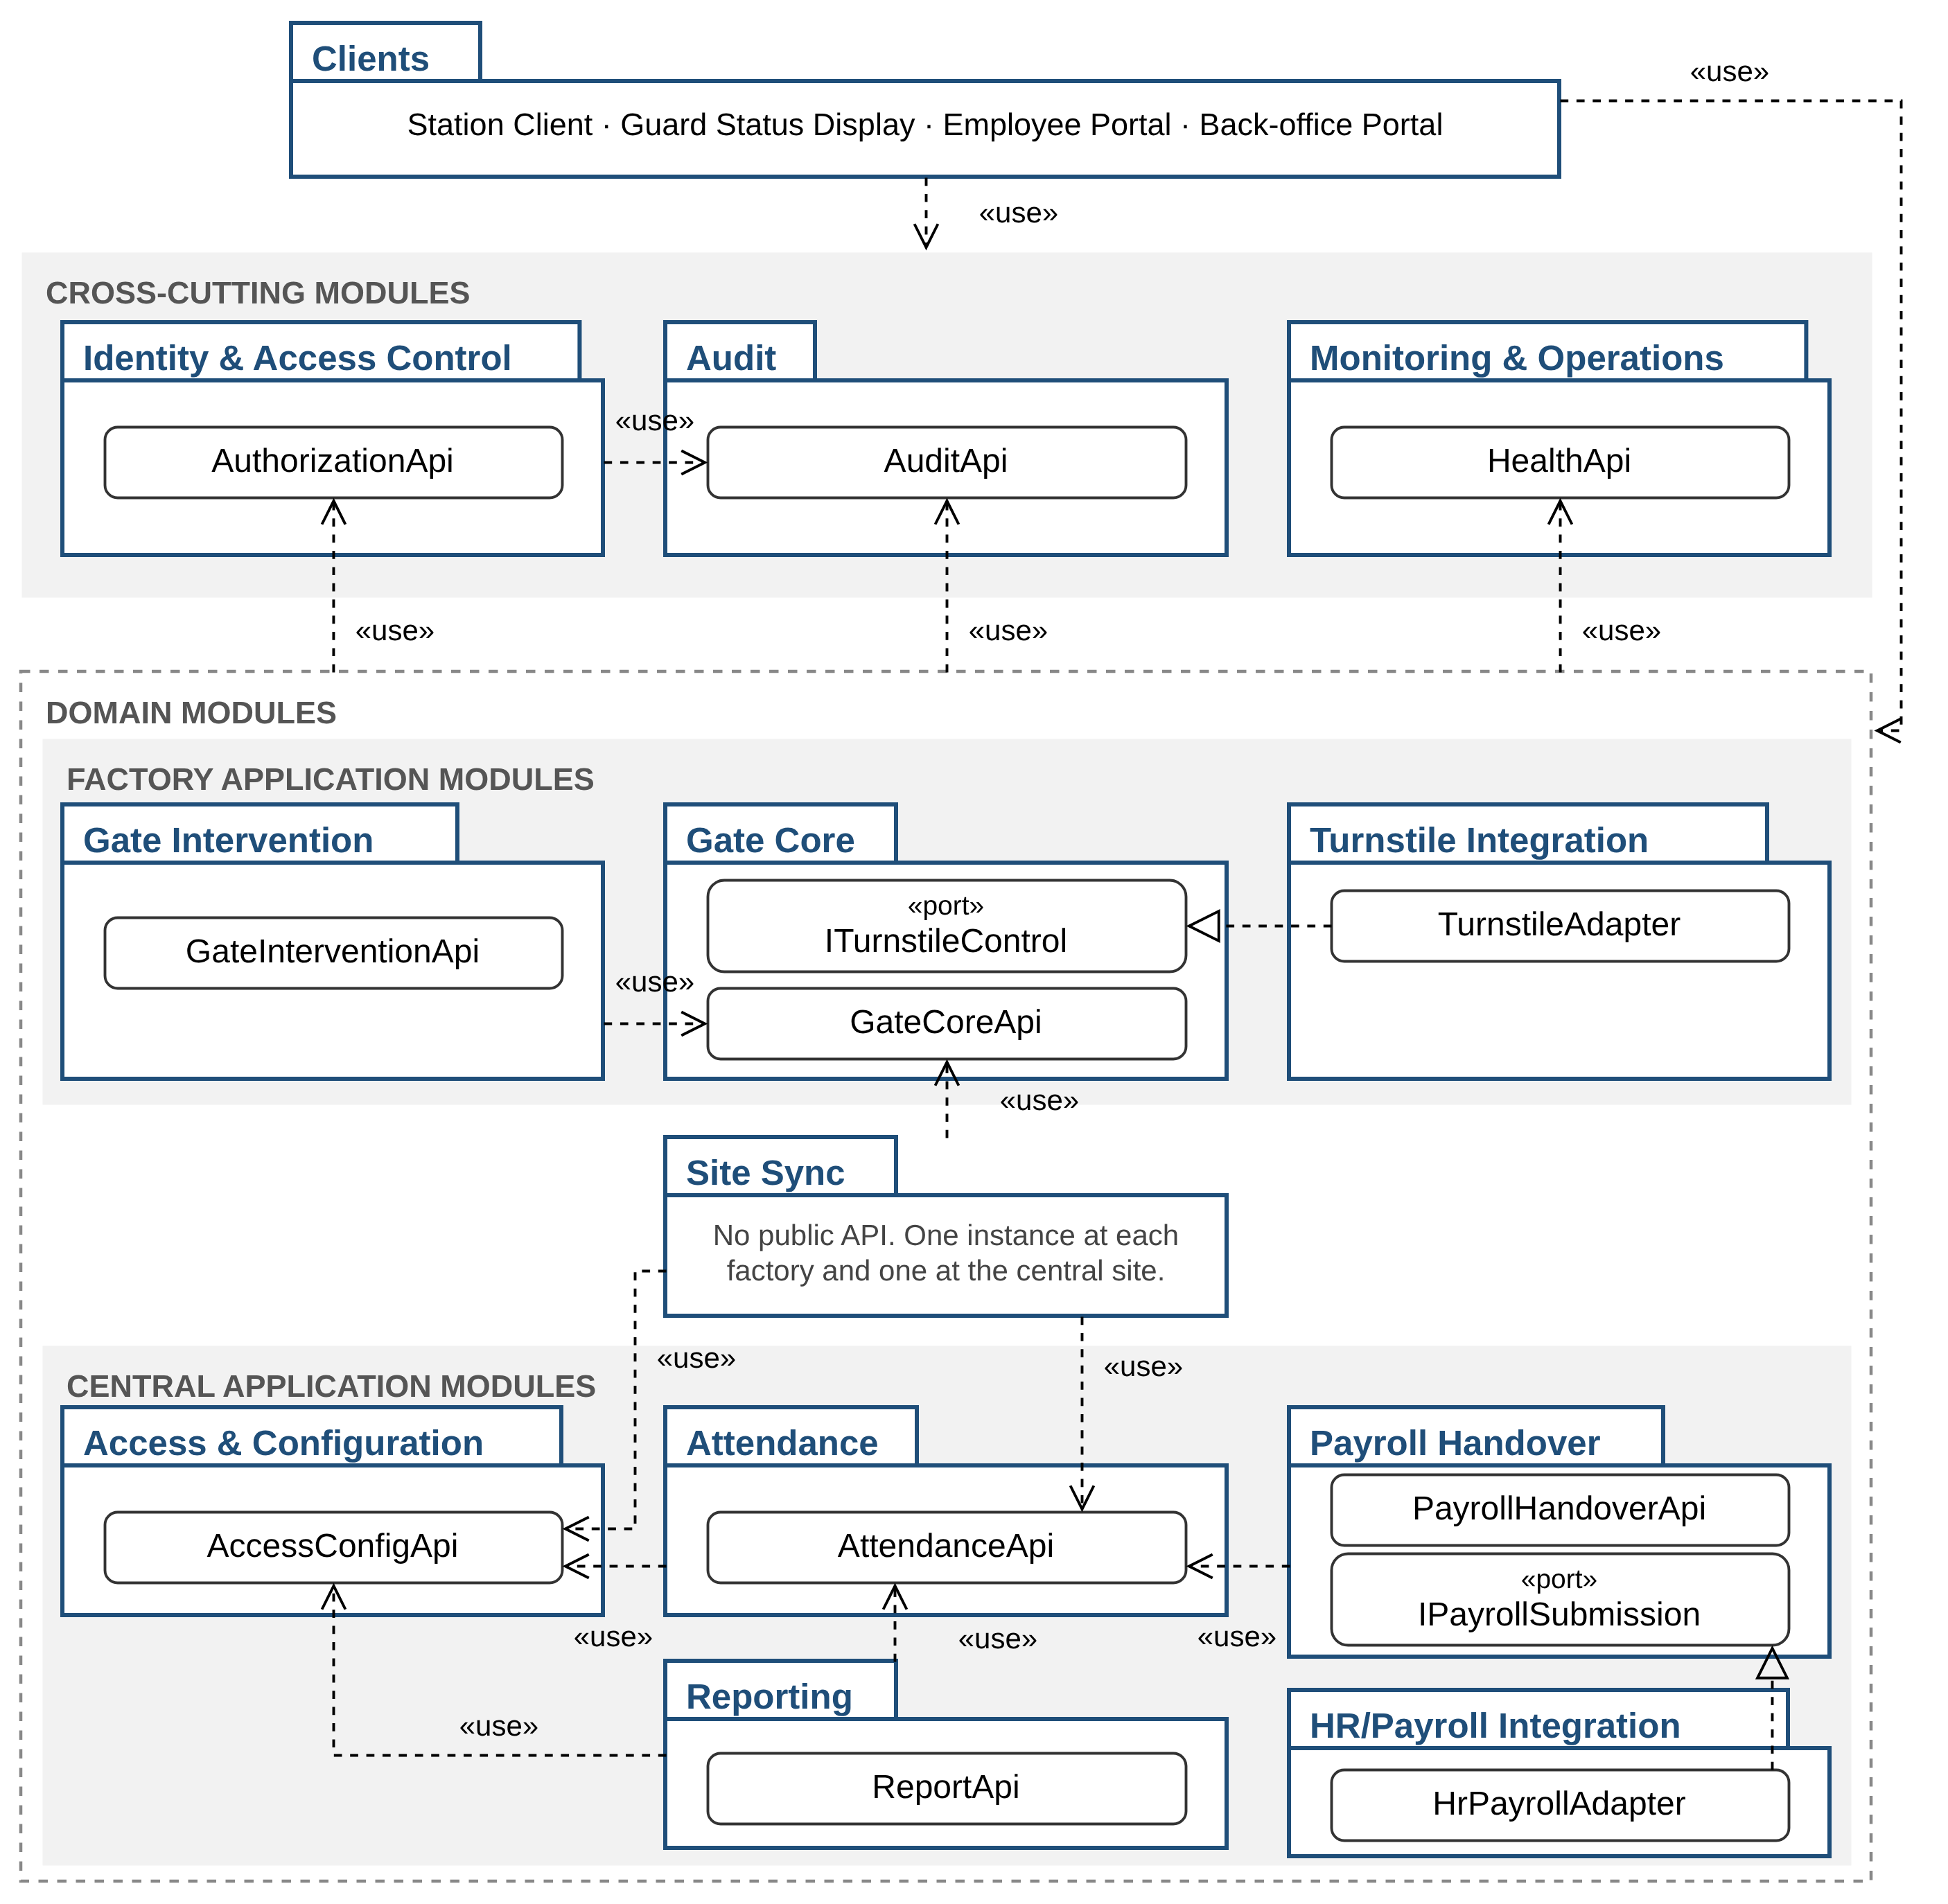
\includegraphics[width=450.0pt,height=463.5pt,keepaspectratio]{diagram/module-view/figure-4-1-module-view.png}

\end{center}

\begin{center}

\textbf{Figure 4.1. Module View of the TMC System}
\phantomsection\addcontentsline{lof}{figure}{\protect\numberline{4.1}Module View of the TMC System}

\end{center}

\Needspace{6\baselineskip}
Dashed open arrows labelled \guillemotleft use\guillemotright{} show dependencies on public interfaces, not runtime message direction. Dashed arrows with hollow triangles point from adapters to the integration interfaces marked \guillemotleft port\guillemotright{} that they realize. Arrows attached to group boundaries summarize selected dependencies, not dependencies of every module in the group. Table 4.4 lists the exact module pairs.



\begin{longtable}{|>{\raggedright\arraybackslash}p{73.5pt}|>{\raggedright\arraybackslash}p{129.5pt}|>{\raggedright\arraybackslash}p{206.5pt}|}
\hline
\multicolumn{1}{|>{\columncolor{tableheader}\centering\arraybackslash}p{73.5pt}|}{\textbf{Module}} & \multicolumn{1}{>{\columncolor{tableheader}\centering\arraybackslash}p{129.5pt}|}{\textbf{Component}} & \multicolumn{1}{>{\columncolor{tableheader}\centering\arraybackslash}p{206.5pt}|}{\textbf{Responsibility}} \\
\hline
\endhead
\multicolumn{3}{c}{\rule{0pt}{20pt}\normalsize\textbf{Table 4.3. Modules and Responsibilities after Restructuring}} \\
\endlastfoot
M1 Gate Core & Gate Transaction Processor; Access Decision; Eligibility Snapshot & Coordinate and store scan states; validate QR codes, permissions, and configuration; manage versioned decision-support data. \\
\hline
M2 Turnstile Integration & Turnstile Adapter & Implement the gate control port and translate commands and outcomes according to the Controller API. \\
\hline
M3 Gate Intervention & Gate Intervention & Receive assistance records, authorize assisted and emergency actions, and request Gate Core to store cases and coordinate gate commands. \\
\hline
M4 Access \& Configuration & Access Rights Management; QR Credential Issuance; Email Link Sender; Gate Station Management; Work Schedule Policy & Manage employees, permissions, QR issuance and email display links, station/lane configuration, shift schedules, and aggregation rules. \\
\hline
M5 Attendance & Attendance Consolidation; Attendance Review & Consolidate transactions and apply approved decisions; manage discrepancy reports, assistance cases, reconciliation, and application progress. \\
\hline
M6 Reporting & Reporting & Provide queries, reports, and audit queries within authorized scopes. \\
\hline
M7 Payroll Handover & Payroll Handover & Manage periods, batch content, acknowledgements, errors, and supplementary handovers. \\
\hline
M8 HR/Payroll Integration & HR/Payroll Adapter & Translate data and responses between Payroll Handover and HR/Payroll. \\
\hline
M9 Site Sync & Site Sync & Transfer events and data changes with at-least-once delivery; track progress and processing acknowledgements. \\
\hline
M10 Identity \& Access Control & Identity \& RBAC & Authenticate users and manage sessions, accounts, roles, and permission scopes. \\
\hline
M11 Audit & Audit Log & Receive and store audit records and provide queries through a controlled access path. \\
\hline
M12 Monitoring \& Operations & Monitoring & Monitor operational status, faults, latency, and task progress, and raise alerts. One logical module with a central deployment and a deployment at each factory. \\*
\hline\noalign{\nobreak}
M13 Clients & Station Client; Guard Status Display; Employee Portal; Back-office Portal & Provide station, guard-post status, employee, and management interfaces according to role. \\
\hline
\end{longtable}
\phantomsection\addcontentsline{lot}{table}{\protect\numberline{4.3}Modules and Responsibilities after Restructuring}


\begin{itemize}[leftmargin=36pt, itemsep=2pt, topsep=4pt, parsep=2pt]
  \item \textbf{Responsibility boundaries.} In the automatic QR flow, Gate Transaction Processor creates transactions. For assistance and reconciliation, Attendance Review stores the decision, Attendance Consolidation applies it to attendance, and Gate Core updates the scan. Gate Core defines the turnstile command ports and IPassageEvents. Turnstile Adapter implements the command ports and calls IPassageEvents to report passage and lane-clear events. Payroll Handover defines IPayrollSubmission, implemented by HR/Payroll Adapter.
  \item \textbf{Inside each module.} Data-owning business modules use three layers: an entry layer (API controller, event handler, or scheduled trigger), a business layer whose facade implements the module's public interface, and a persistence layer with its repositories and the ports it defines. Gate Intervention and Reporting own no business data, so they have no persistence layer and call the owning module's interface instead. Audit and Monitoring receive calls directly at their facade and have no separate entry layer. Site Sync uses background workers and exposes no public facade. Adapters and clients keep their own simpler structure. Other modules call only the facade, never the services or repositories behind it.
\end{itemize}

\Needspace{9\baselineskip}
\subsubsection*{4.1.3. Module Dependencies}

\phantomsection
\addcontentsline{toc}{subsubsection}{4.1.3. Module Dependencies}


Table 4.4 shows which modules each module depends on and the reason for each dependency.

\begin{longtable}{|>{\raggedright\arraybackslash}p{45.5pt}|>{\raggedright\arraybackslash}p{100.5pt}|>{\raggedright\arraybackslash}p{263.5pt}|}
\hline
\multicolumn{1}{|>{\columncolor{tableheader}\centering\arraybackslash}p{45.5pt}|}{\textbf{Module}} & \multicolumn{1}{>{\columncolor{tableheader}\centering\arraybackslash}p{100.5pt}|}{\textbf{Depends On}} & \multicolumn{1}{>{\columncolor{tableheader}\centering\arraybackslash}p{263.5pt}|}{\textbf{Purpose}} \\
\hline
\endhead
\multicolumn{3}{c}{\rule{0pt}{20pt}\normalsize\textbf{Table 4.4. Module Dependencies}} \\
\endlastfoot
M1 & M11, M12 & Transfer audit and operational information. \\
\hline
M2 & M1, M12 & Implement the turnstile command ports defined by Gate Core, pass PASSAGE and LANE\_CLEAR to Gate Core through IPassageEvents, and report integration status. \\
\hline
M3 & M1, M10, M11 & Record cases, use the control port, check authorization, and record audit evidence. \\
\hline
M4 & M10, M11 & Check authorization and record change histories. \\
\hline
M5 & M4, M10, M11 & Use aggregation rules, check authorization, and record audit evidence. \\
\hline
M6 & M4, M5, M10, M11 & Obtain rules and attendance data, check scope, and query audit records. \\
\hline
M7 & M5, M10, M11, M12 & Obtain period data and cases, check authorization, record audit evidence, and raise alerts. \\
\hline
M8 & M7 & Implement IPayrollSubmission. \\
\hline
M9 & M1, M4, M5, M11, M12 & Use data exchange contracts, record evidence, and monitor synchronization. \\
\hline
M10 & M11 & Record authentication and permission change evidence. \\
\hline
M11 & No business module dependencies & Receive and provide audit data. \\
\hline
M12 & No business module dependencies & Receive operational information. \\*
\hline\noalign{\nobreak}
M13 & M1, M3, M4, M5, M6, M7, M10, M12 & Access functions through public interfaces. \\
\hline
\end{longtable}
\phantomsection\addcontentsline{lot}{table}{\protect\numberline{4.4}Module Dependencies}


For example, Gate Transaction Processor calls Turnstile Adapter at runtime, but in the contract graph Turnstile Integration depends on the port defined by Gate Core.

\Needspace{6\baselineskip}
The modules follow these dependency rules:

\begin{itemize}[leftmargin=36pt, itemsep=2pt, topsep=4pt, parsep=2pt]

  \item Other modules are reached only through their public interfaces, never through their internal components or data.

  \item Only the data owner updates its data; others send requests through its interface.

  \item The dependencies in Table 4.4 have no cycles.

  \item Reporting checks authorization through Identity \& RBAC before querying Audit Log, and Audit Log never calls back, which avoids a cycle.

  \item Gate Core and Turnstile Integration do not depend on Reporting, Payroll Handover, HR/Payroll Integration, or Attendance, so the kiosk does not wait for these modules. Interference through shared resources still needs limits and performance tests.

\end{itemize}

\Needspace{9\baselineskip}
\subsubsection*{4.1.4. FR Coverage after Restructuring}

\phantomsection
\addcontentsline{toc}{subsubsection}{4.1.4. FR Coverage after Restructuring}


Table 4.5 gives the main and supporting components for each of the 26 functional requirements.

\begin{longtable}{|>{\raggedright\arraybackslash}p{41.5pt}|>{\raggedright\arraybackslash}p{187.5pt}|>{\raggedright\arraybackslash}p{179.5pt}|}
\hline
\multicolumn{1}{|>{\columncolor{tableheader}\centering\arraybackslash}p{41.5pt}|}{\textbf{FR}} & \multicolumn{1}{>{\columncolor{tableheader}\centering\arraybackslash}p{187.5pt}|}{\textbf{Primarily Responsible Components}} & \multicolumn{1}{>{\columncolor{tableheader}\centering\arraybackslash}p{179.5pt}|}{\textbf{Collaborating Components}} \\
\hline
\endhead
\multicolumn{3}{c}{\rule{0pt}{20pt}\normalsize\textbf{Table 4.5. FR-to-Component Mapping after Restructuring}} \\
\endlastfoot
FR-01.1 & Access Rights Management & Identity \& RBAC; Back-office Portal \\
\hline
FR-01.2 & QR Credential Issuance; Access Decision & Eligibility Snapshot \\
\hline
FR-01.3 & QR Credential Issuance; Email Link Sender & Employee Portal; Identity \& RBAC; TMC email service \\
\hline
FR-01.4 & Access Rights Management & Site Sync; Eligibility Snapshot; Identity \& RBAC \\
\hline
FR-02.1 & Gate Station Management & Site Sync; Eligibility Snapshot \\
\hline
FR-02.2 & Gate Transaction Processor; Turnstile Adapter & --- \\
\hline
FR-02.3 & Monitoring & Station Client; Turnstile Adapter; Gate Transaction Processor \\
\hline
FR-02.4 & Gate Intervention & Identity \& RBAC; Gate Transaction Processor; Turnstile Adapter; Audit Log \\
\hline
FR-03.1 & Station Client; Gate Transaction Processor & Access Decision \\
\hline
FR-03.2 & Access Decision & Eligibility Snapshot; Access Rights Management \\
\hline
FR-03.3 & Gate Transaction Processor; Attendance Consolidation & Turnstile Adapter; Site Sync; Attendance Review \\
\hline
FR-03.4 & Gate Transaction Processor; Attendance Consolidation & Station Client; Site Sync \\
\hline
FR-03.5 & Gate Transaction Processor; Attendance Consolidation & Gate Station Management; Eligibility Snapshot \\
\hline
FR-03.6 & Gate Transaction Processor & Site Sync; Attendance Review; Audit Log \\
\hline
FR-04.1 & Reporting & Attendance Consolidation; Identity \& RBAC \\
\hline
FR-04.2 & Reporting & Attendance Consolidation; Work Schedule Policy \\
\hline
FR-04.3 & Payroll Handover; HR/Payroll Adapter & Attendance Consolidation; Attendance Review; Monitoring \\
\hline
FR-04.4 & Attendance Review; Attendance Consolidation & Employee Portal; Back-office Portal; Identity \& RBAC; Audit Log \\
\hline
FR-04.5 & Audit Log & Components originating business and administrative actions \\
\hline
FR-04.6 & Reporting & Attendance Consolidation; Identity \& RBAC; Employee Portal; Back-office Portal \\
\hline
FR-04.7 & Reporting; Audit Log & Identity \& RBAC \\
\hline
FR-05.1 & Identity \& RBAC & Back-office Portal; Audit Log \\
\hline
FR-05.2 & Work Schedule Policy & Back-office Portal; Identity \& RBAC \\
\hline
FR-05.3 & Monitoring & Station Client; Turnstile Adapter; Gate Transaction Processor; Site Sync; Payroll Handover \\
\hline
FR-05.4 & Monitoring and operational mechanisms of data-owning components & Data-owning modules \\*
\hline\noalign{\nobreak}
FR-05.5 & Identity \& RBAC & Employee Portal; Back-office Portal; Audit Log \\
\hline
\end{longtable}
\phantomsection\addcontentsline{lot}{table}{\protect\numberline{4.5}FR-to-Component Mapping after Restructuring}


\Needspace{9\baselineskip}
\subsubsection*{4.1.5. Driving Characteristic Coverage}

\phantomsection
\addcontentsline{toc}{subsubsection}{4.1.5. Driving Characteristic Coverage}


Table 4.6 shows which design mechanisms support each driving characteristic.

\begin{longtable}{|>{\raggedright\arraybackslash}p{92.5pt}|>{\raggedright\arraybackslash}p{82.5pt}|>{\raggedright\arraybackslash}p{234.5pt}|}
\hline
\multicolumn{1}{|>{\columncolor{tableheader}\centering\arraybackslash}p{92.5pt}|}{\textbf{Characteristic}} & \multicolumn{1}{>{\columncolor{tableheader}\centering\arraybackslash}p{82.5pt}|}{\textbf{Related Requirements}} & \multicolumn{1}{>{\columncolor{tableheader}\centering\arraybackslash}p{234.5pt}|}{\textbf{Design Mechanism}} \\
\hline
\endhead
\multicolumn{3}{c}{\rule{0pt}{20pt}\normalsize\textbf{Table 4.6. Driving Characteristics Covered by the Logical Design}} \\
\endlastfoot
AC-01 Reliability/Data Integrity & NFR-02; FR-03.3--FR-03.6; I-03 & Gate Transaction Processor owns durable recording and scan states; Attendance Consolidation blocks duplicates; undetermined outcomes are kept for inquiry. \\
\hline
AC-02 Availability & FR-02.3; FR-05.3 & Monitoring detects outages; components recover from stored states and events. Local access data may be used only for a limited time (I-10). \\
\hline
AC-03 Performance & NFR-01; IC-02 & Only Gate Transaction Processor, Access Decision, Eligibility Snapshot, and Turnstile Adapter sit on the kiosk path; reporting and handover do not. \\
\hline
AC-04 Security/Privacy & NFR-03; NFR-04; FR-01.2; FR-03.2; FR-05.5; I-04 & Identity \& RBAC controls actions and data scope; QR codes and screens show minimal personal data; HR approves assistance cases. \\
\hline
AC-05 Auditability & NFR-03; FR-04.4; FR-04.5; FR-04.7; I-04 & Evidence is stored at its source and sent to Audit Log; cases, decisions, and handovers are linked; audit queries are authorized first. \\*
\hline\noalign{\nobreak}
AC-06 Interoperability & FR-02.2; FR-04.3; IC-01; IC-02; I-01--I-03; I-05; I-07 & Two ports and adapters isolate the external APIs and interpret their signals and acknowledgements. \\
\hline
\end{longtable}
\phantomsection\addcontentsline{lot}{table}{\protect\numberline{4.6}Driving Characteristics Covered by the Logical Design}


\Needspace{9\baselineskip}
\subsubsection*{4.1.6. Inside the Modules}

\phantomsection
\addcontentsline{toc}{subsubsection}{4.1.6. Inside the Modules}


Figures 4.2--4.14 show the inside of each module. These figures are UML-inspired module views: they show the static decomposition and the dependencies between parts, not the order of runtime messages. They use this notation:

\begin{itemize}[leftmargin=36pt, itemsep=2pt, topsep=4pt, parsep=2pt]
  \item A dashed open arrow labelled \guillemotleft use\guillemotright{} means that one part depends on another.
  \item The facade implements the module's public interface; this is drawn as a dashed arrow ending in a hollow triangle.
  \item A box marked \guillemotleft port\guillemotright{} is an integration interface that the module owns and an adapter implements; this is our own label, not a UML port.
  \item Each frame is divided into \guillemotleft layer\guillemotright{} areas (Entry, Business, Persistence) where the module has them.
  \item Dashed boxes outside a module frame are public interfaces of other modules, such as AuditApi, or external APIs and systems, such as the Controller API or the HR/Payroll API.
\end{itemize}

The component names below module level are our proposed decomposition. Table 4.3 stays the reference for module responsibilities, and Tables 4.7--4.19 under the figures only explain their components.

\textbf{Names in the figures.} Names without spaces, such as GateTransactionProcessor, refer to the same parts as their spaced names in the text; each module's figure and table show any further decomposition.

\noindent\begin{minipage}{\linewidth}
Figure 4.2 shows the inside of Gate Core, and Table 4.7 describes its components.

\vspace{6pt}
\centering
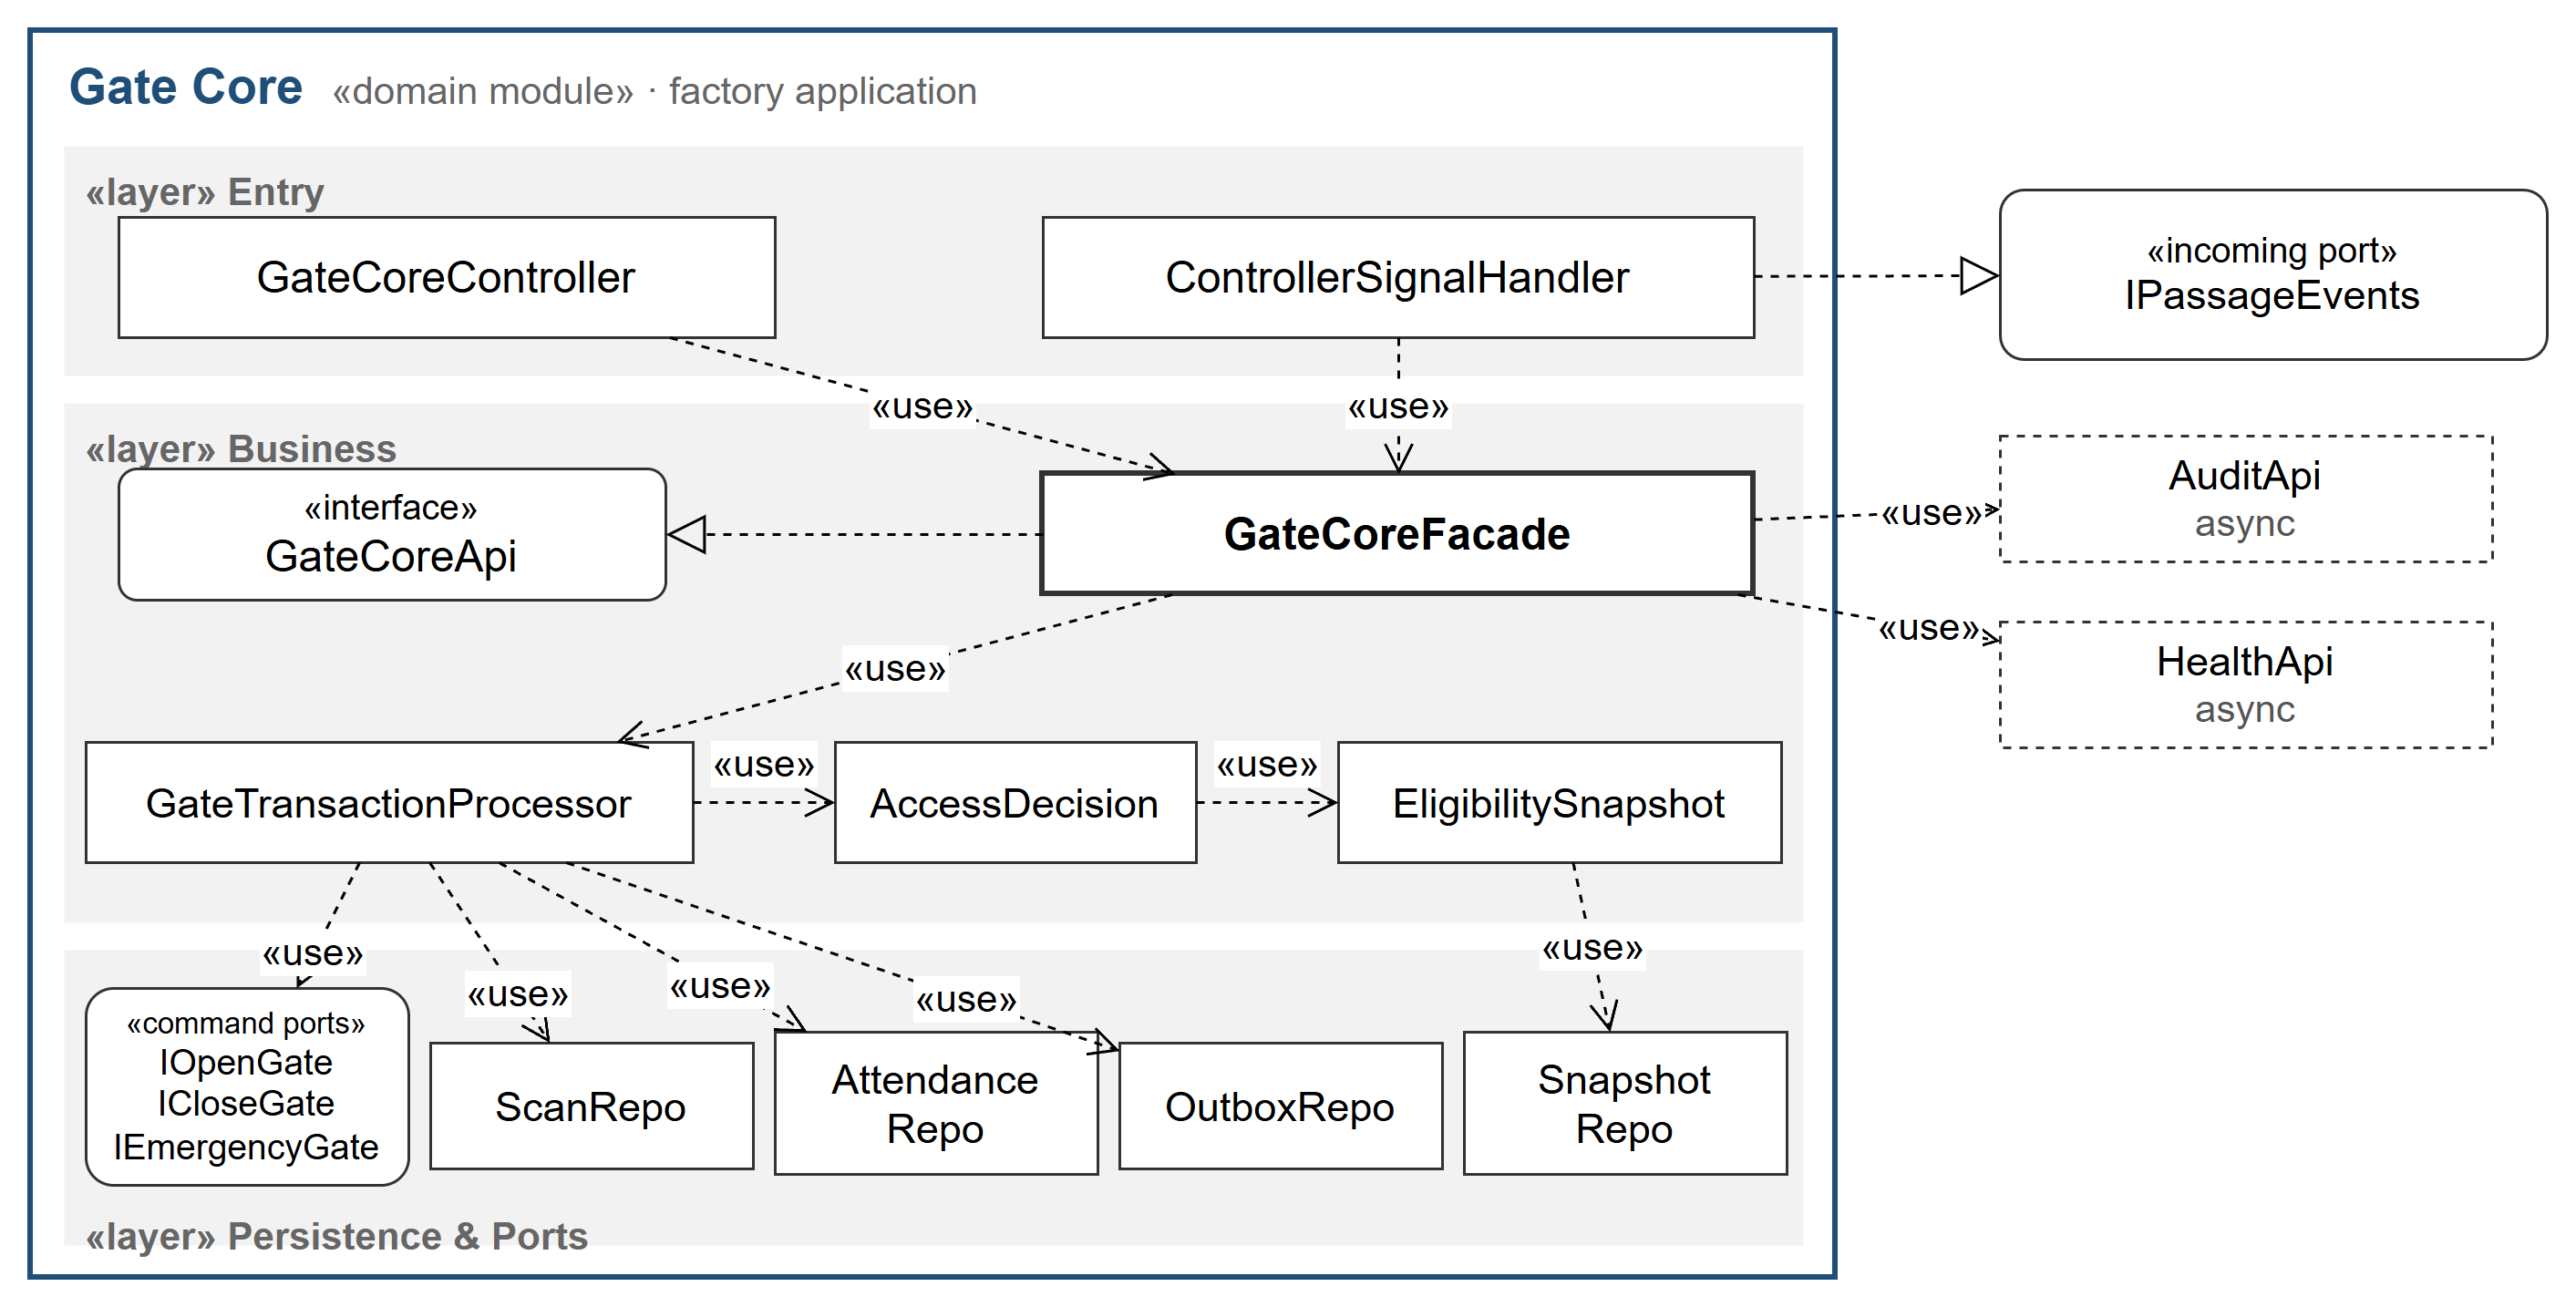
\includegraphics[width=435.8pt]{diagram/modules/figure-4-2-m1.png}

\vspace{6pt}
\textbf{Figure 4.2. M1 Gate Core}
\phantomsection\addcontentsline{lof}{figure}{\protect\numberline{4.2}M1 Gate Core}

\vspace{8pt}
{\small
\begin{tabular}{|>{\raggedright\arraybackslash}p{120pt}|>{\raggedright\arraybackslash}p{290pt}|}
\hline
\multicolumn{1}{|>{\columncolor{tableheader}\centering\arraybackslash}p{120pt}|}{\textbf{Component}} & \multicolumn{1}{>{\columncolor{tableheader}\centering\arraybackslash}p{290pt}|}{\textbf{Responsibility}} \\
\hline
GateCoreController & Receives scans from Station Client, guard actions from Gate Intervention, and access changes and resolutions from Site Sync. \\
\hline
ControllerSignalHandler & Receives PASSAGE and LANE\_CLEAR for a lane and command through IPassageEvents, which Gate Core implements and Turnstile Integration calls. OPEN\_CONFIRMED and CLOSED are not callbacks; they come back as the results of openGate and closeGate. \\
\hline
GateTransactionProcessor & Keeps scan and gate-cycle states, reserves the lane, sends controller commands, and creates attendance only after passage. \\
\hline
AccessDecision, EligibilitySnapshot & Check whether the versioned access data is usable, select normal or degraded mode (I-10), and check the QR code, permission, and configuration. Return CANNOT PROCESS when the required data cannot be used. \\
\hline
Repositories & ScanRepo and AttendanceRepo hold the original factory records. OutboxRepo stores Gate Event Feed events and audit evidence in the same transaction; audit and health data leave asynchronously, never on the scan path. \\
\hline
\end{tabular}
}

\vspace{6pt}
\textbf{Table 4.7. Components of M1 Gate Core}
\phantomsection\addcontentsline{lot}{table}{\protect\numberline{4.7}Components of M1 Gate Core}
\end{minipage}

\vspace{14pt}

\noindent\begin{minipage}{\linewidth}
Figure 4.3 shows the inside of Turnstile Integration, and Table 4.8 describes its components.

\vspace{6pt}
\centering
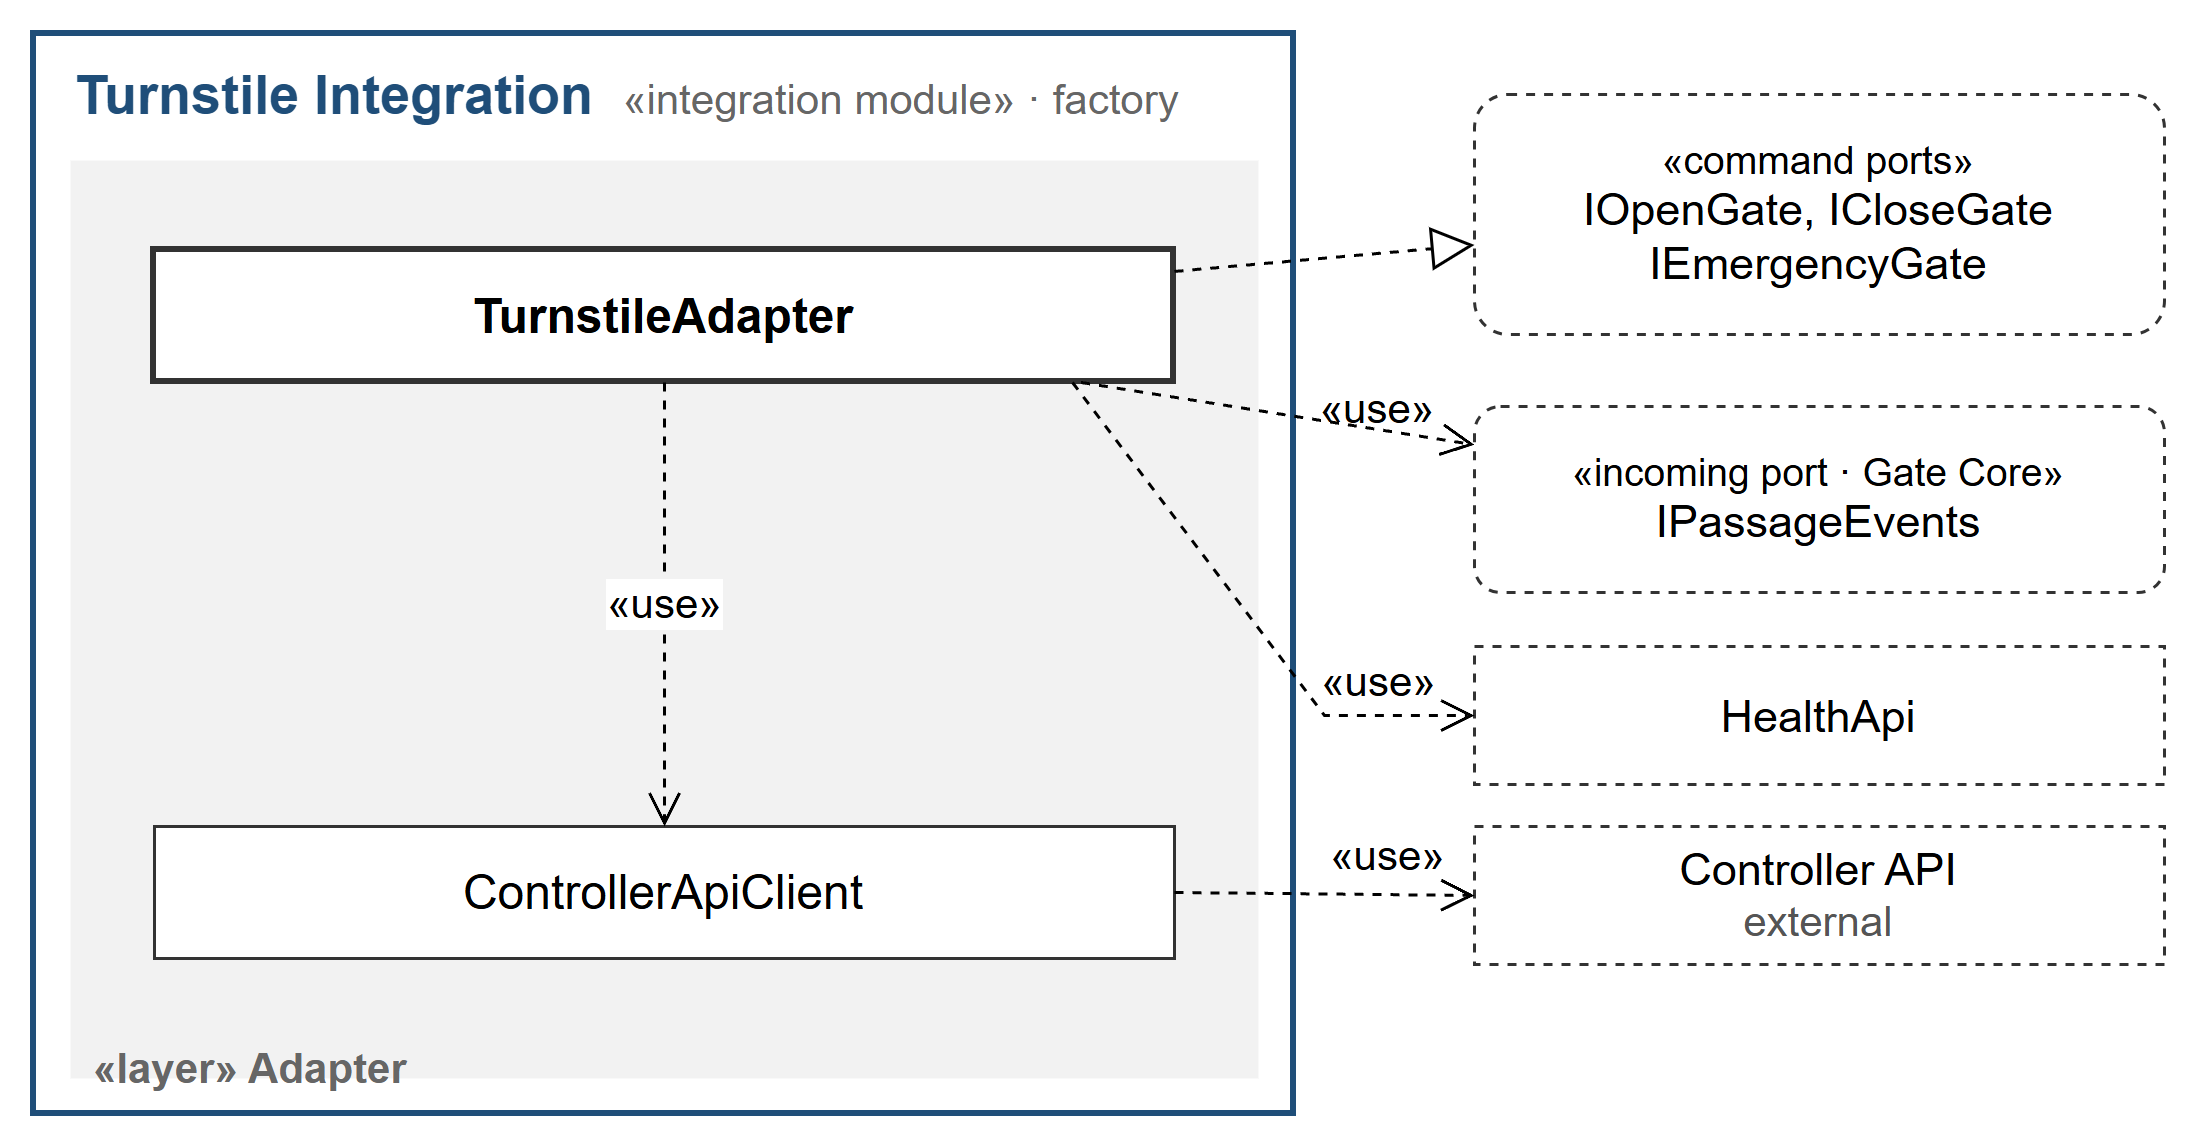
\includegraphics[width=345.6pt]{diagram/modules/figure-4-3-m2.png}

\vspace{6pt}
\textbf{Figure 4.3. M2 Turnstile Integration}
\phantomsection\addcontentsline{lof}{figure}{\protect\numberline{4.3}M2 Turnstile Integration}

\vspace{8pt}
{\small
\begin{tabular}{|>{\raggedright\arraybackslash}p{120pt}|>{\raggedright\arraybackslash}p{290pt}|}
\hline
\multicolumn{1}{|>{\columncolor{tableheader}\centering\arraybackslash}p{120pt}|}{\textbf{Component}} & \multicolumn{1}{>{\columncolor{tableheader}\centering\arraybackslash}p{290pt}|}{\textbf{Responsibility}} \\
\hline
TurnstileAdapter & Implements the command ports IOpenGate, ICloseGate, and IEmergencyGate (and the status query where the API has one), translates commands and results, and keeps ``received'', ``opened'', and ``uncertain'' apart. It forwards PASSAGE and LANE\_CLEAR to Gate Core through IPassageEvents. \\
\hline
ControllerApiClient & Calls the Controller API and receives its signals (I-01, I-05). \\
\hline
\end{tabular}
}

\vspace{6pt}
\textbf{Table 4.8. Components of M2 Turnstile Integration}
\phantomsection\addcontentsline{lot}{table}{\protect\numberline{4.8}Components of M2 Turnstile Integration}
\end{minipage}

\vspace{14pt}

\noindent\begin{minipage}{\linewidth}
Figure 4.4 shows the inside of Gate Intervention, and Table 4.9 describes its components.

\vspace{6pt}
\centering
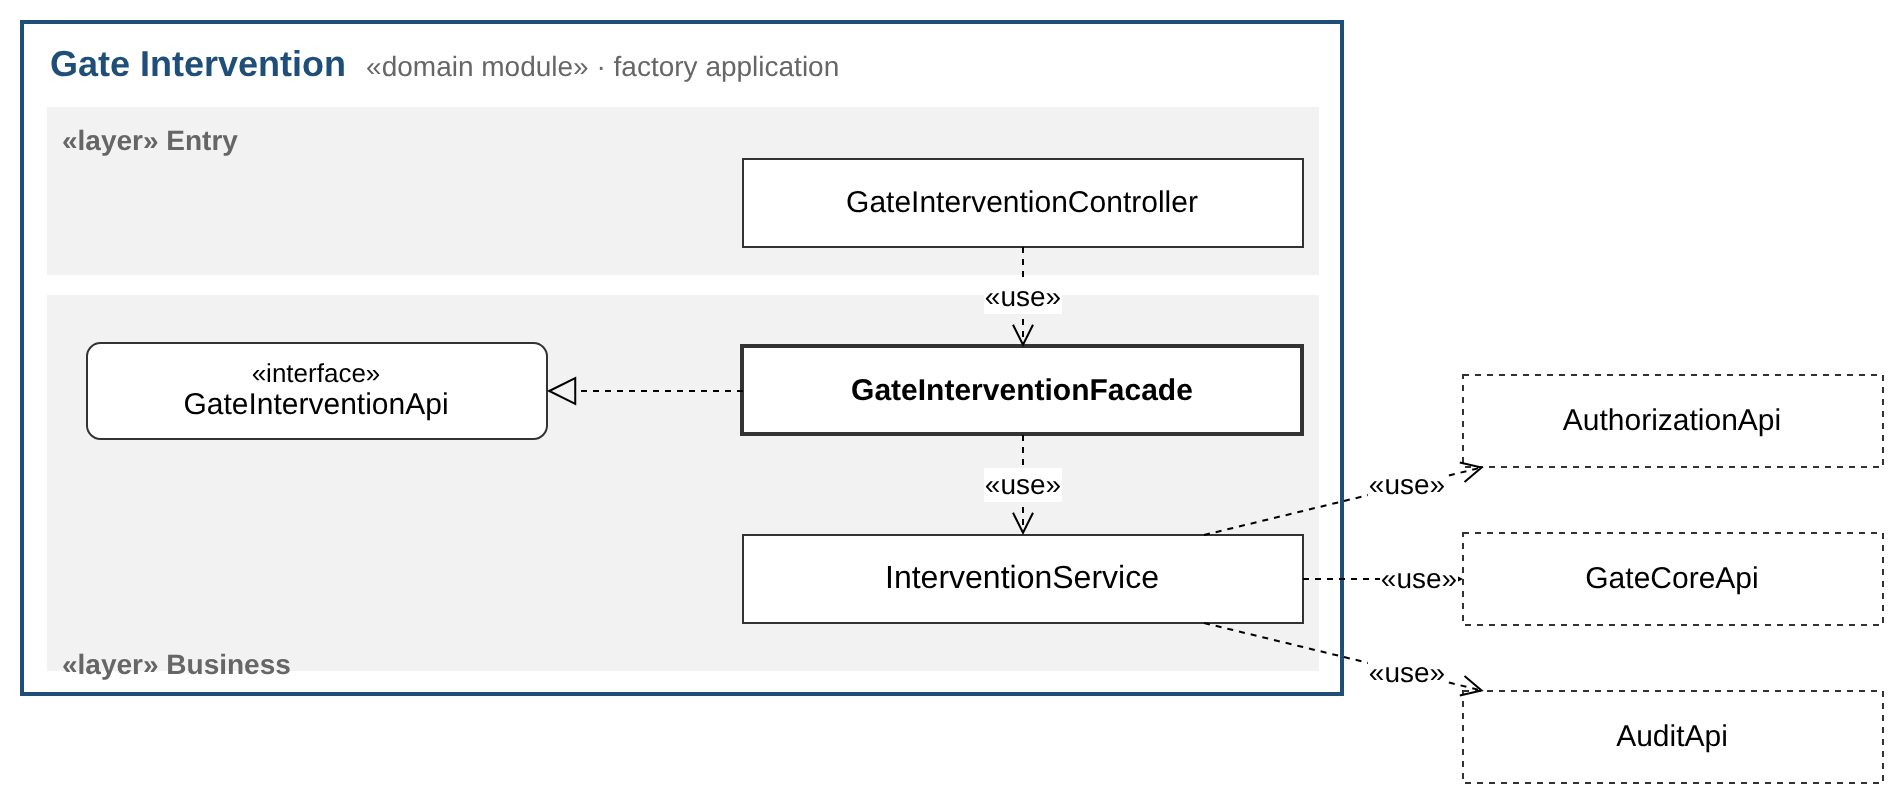
\includegraphics[width=450pt]{diagram/modules/figure-4-4-m3.png}

\vspace{6pt}
\textbf{Figure 4.4. M3 Gate Intervention}
\phantomsection\addcontentsline{lof}{figure}{\protect\numberline{4.4}M3 Gate Intervention}

\vspace{8pt}
{\small
\begin{tabular}{|>{\raggedright\arraybackslash}p{120pt}|>{\raggedright\arraybackslash}p{290pt}|}
\hline
\multicolumn{1}{|>{\columncolor{tableheader}\centering\arraybackslash}p{120pt}|}{\textbf{Component}} & \multicolumn{1}{>{\columncolor{tableheader}\centering\arraybackslash}p{290pt}|}{\textbf{Responsibility}} \\
\hline
GateInterventionController, Facade & Receive guard actions from Back-office Portal and implement GateInterventionApi. \\
\hline
InterventionService & Checks the guard's authority, assigns the supportCaseId, and asks Gate Core to store the case and open or release the gate. It owns no business data. \\
\hline
\end{tabular}
}

\vspace{6pt}
\textbf{Table 4.9. Components of M3 Gate Intervention}
\phantomsection\addcontentsline{lot}{table}{\protect\numberline{4.9}Components of M3 Gate Intervention}
\end{minipage}

\vspace{14pt}

\noindent\begin{minipage}{\linewidth}
Figure 4.5 shows the inside of Access \& Configuration, and Table 4.10 describes its components.

\vspace{6pt}
\centering
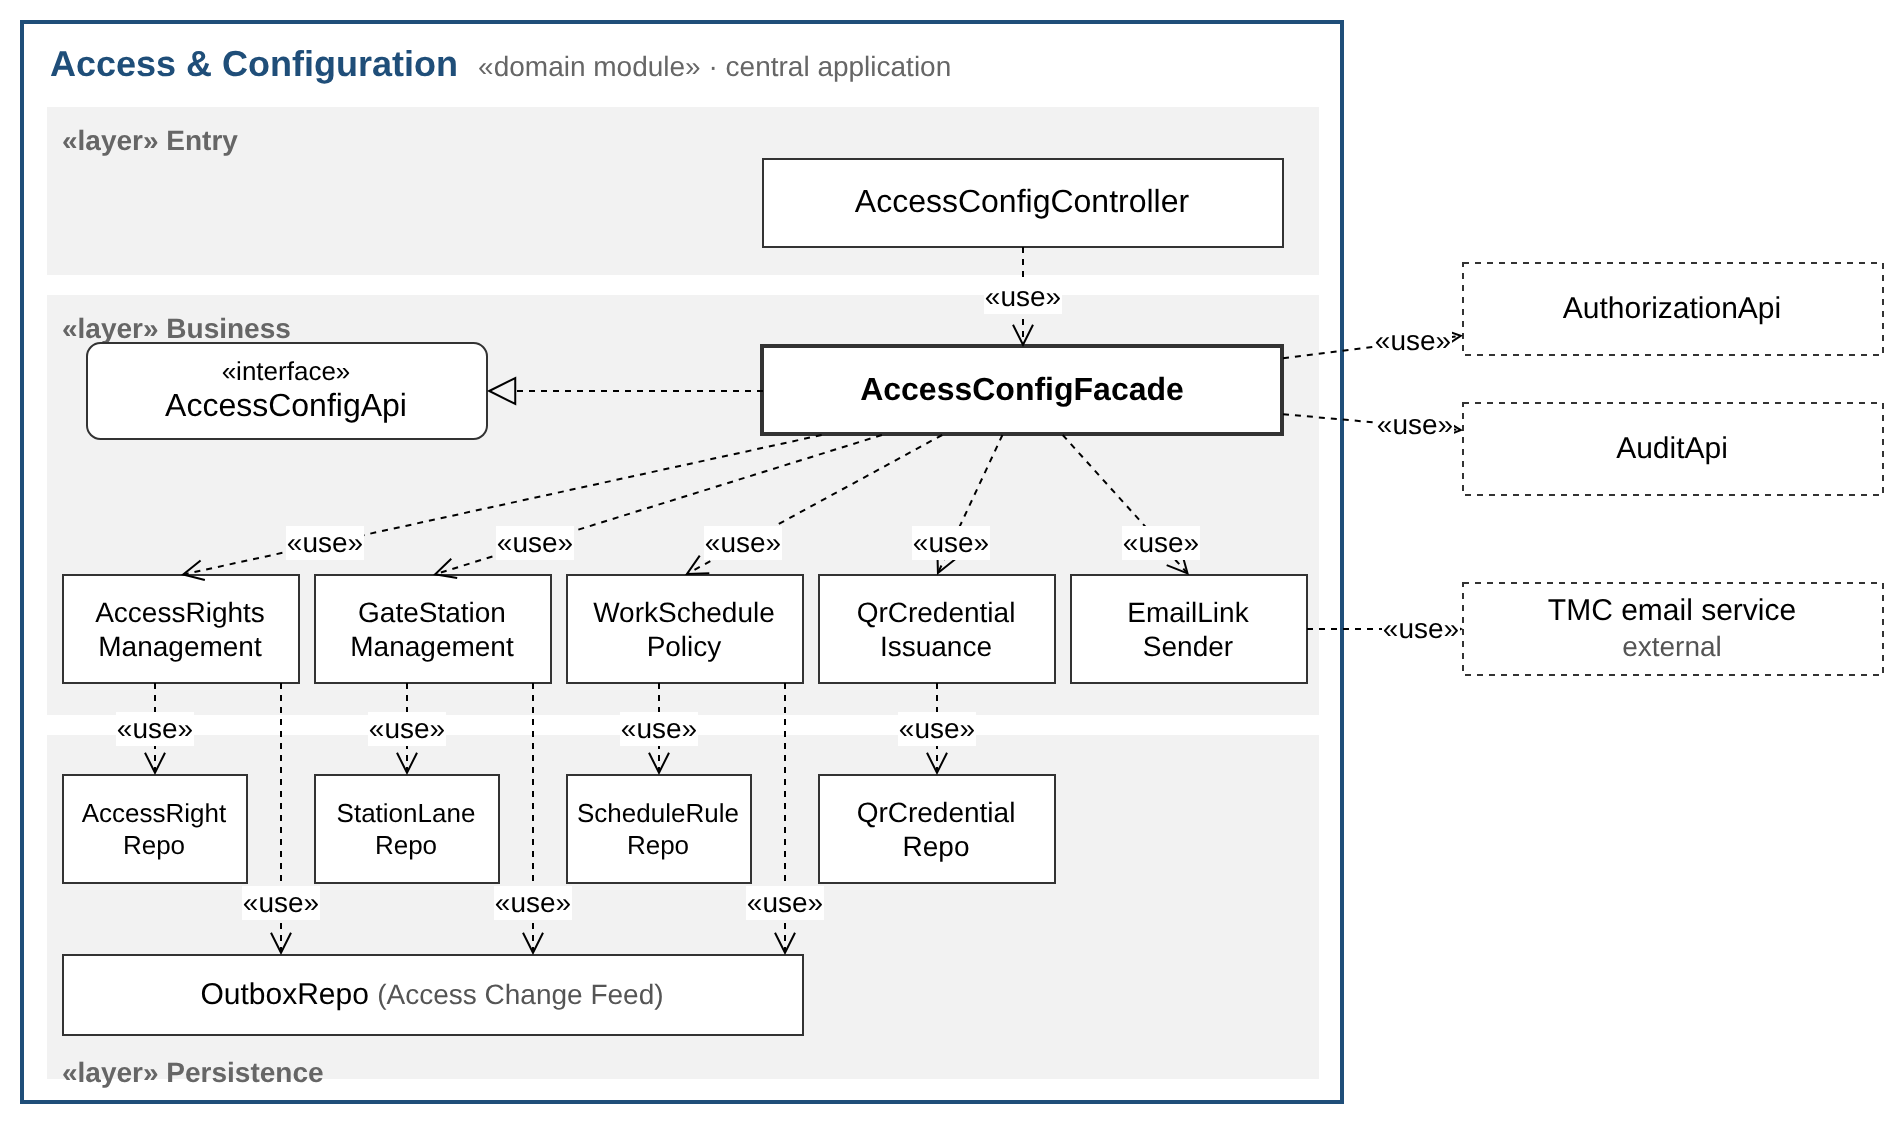
\includegraphics[width=450pt]{diagram/modules/figure-4-5-m4.png}

\vspace{6pt}
\textbf{Figure 4.5. M4 Access \& Configuration}
\phantomsection\addcontentsline{lof}{figure}{\protect\numberline{4.5}M4 Access \& Configuration}

\vspace{8pt}
{\small
\begin{tabular}{|>{\raggedright\arraybackslash}p{120pt}|>{\raggedright\arraybackslash}p{290pt}|}
\hline
\multicolumn{1}{|>{\columncolor{tableheader}\centering\arraybackslash}p{120pt}|}{\textbf{Component}} & \multicolumn{1}{>{\columncolor{tableheader}\centering\arraybackslash}p{290pt}|}{\textbf{Responsibility}} \\
\hline
AccessRightsManagement & Manages employees and their permissions. \\
\hline
QrCredentialIssuance & Issues signed, single-use QR codes that expire after 60 seconds (ADR-11). \\
\hline
GateStationManagement, WorkSchedulePolicy & Manage stations and lanes, shifts, and aggregation rules. \\
\hline
EmailLinkSender & Sends a link to the QR screen, never the QR image (I-08). \\
\hline
OutboxRepo & Stores Access Change Feed events in the same transaction as each change. \\
\hline
\end{tabular}
}

\vspace{6pt}
\textbf{Table 4.10. Components of M4 Access \& Configuration}
\phantomsection\addcontentsline{lot}{table}{\protect\numberline{4.10}Components of M4 Access \& Configuration}
\end{minipage}

\vspace{14pt}

\noindent\begin{minipage}{\linewidth}
Figure 4.6 shows the inside of Attendance, and Table 4.11 describes its components.

\vspace{6pt}
\centering
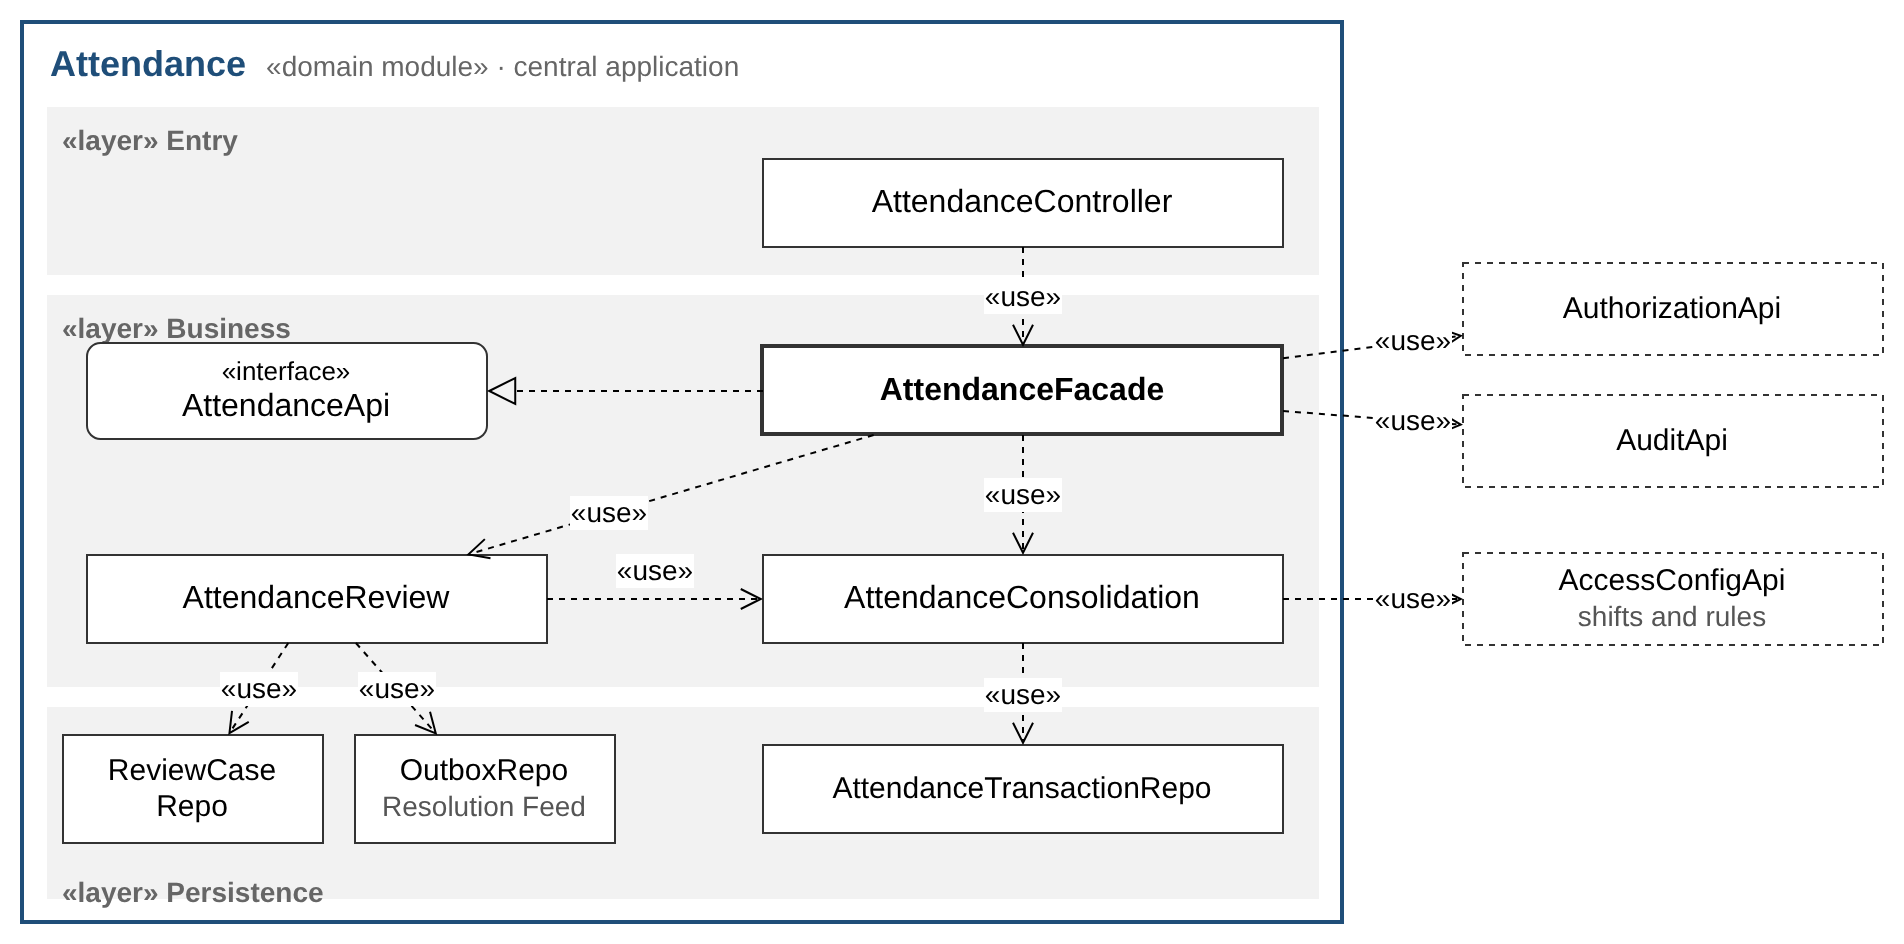
\includegraphics[width=450pt]{diagram/modules/figure-4-6-m5.png}

\vspace{6pt}
\textbf{Figure 4.6. M5 Attendance}
\phantomsection\addcontentsline{lof}{figure}{\protect\numberline{4.6}M5 Attendance}

\vspace{8pt}
{\small
\begin{tabular}{|>{\raggedright\arraybackslash}p{120pt}|>{\raggedright\arraybackslash}p{290pt}|}
\hline
\multicolumn{1}{|>{\columncolor{tableheader}\centering\arraybackslash}p{120pt}|}{\textbf{Component}} & \multicolumn{1}{>{\columncolor{tableheader}\centering\arraybackslash}p{290pt}|}{\textbf{Responsibility}} \\
\hline
AttendanceController, Facade & Implement AttendanceApi and receive Gate Event Feed events delivered by Site Sync. \\
\hline
AttendanceConsolidation & Consolidates transactions and applies approved decisions, using shifts and rules from Access \& Configuration. \\
\hline
AttendanceReview & Handles discrepancy reports, assistance cases, and reconciliation, and writes Resolution Feed events. \\
\hline
Data ownership & Attendance owns consolidated data and adjustments; the original scan records stay in Gate Core. \\
\hline
\end{tabular}
}

\vspace{6pt}
\textbf{Table 4.11. Components of M5 Attendance}
\phantomsection\addcontentsline{lot}{table}{\protect\numberline{4.11}Components of M5 Attendance}
\end{minipage}

\vspace{14pt}

\noindent\begin{minipage}{\linewidth}
Figure 4.7 shows the inside of Reporting, and Table 4.12 describes its components.

\vspace{6pt}
\centering
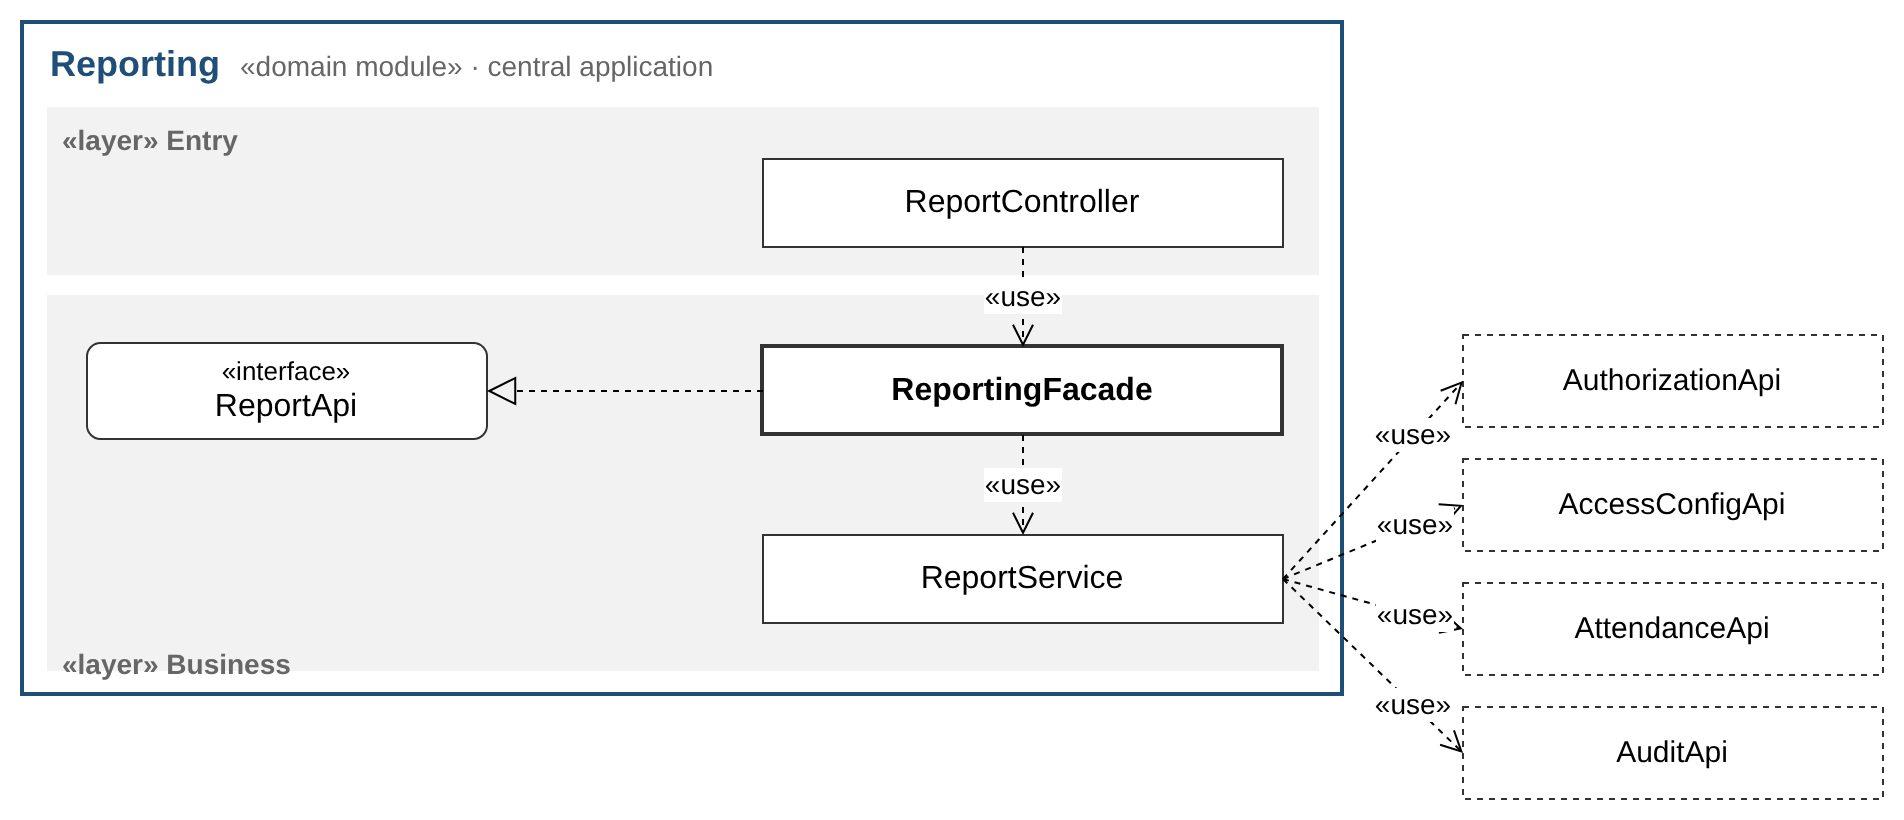
\includegraphics[width=450pt]{diagram/modules/figure-4-7-m6.png}

\vspace{6pt}
\textbf{Figure 4.7. M6 Reporting}
\phantomsection\addcontentsline{lof}{figure}{\protect\numberline{4.7}M6 Reporting}

\vspace{8pt}
{\small
\begin{tabular}{|>{\raggedright\arraybackslash}p{120pt}|>{\raggedright\arraybackslash}p{290pt}|}
\hline
\multicolumn{1}{|>{\columncolor{tableheader}\centering\arraybackslash}p{120pt}|}{\textbf{Component}} & \multicolumn{1}{>{\columncolor{tableheader}\centering\arraybackslash}p{290pt}|}{\textbf{Responsibility}} \\
\hline
ReportController, Facade & Implement ReportApi for both portals. \\
\hline
ReportService & Checks the scope through AuthorizationApi first, then reads access, attendance, and audit data. It keeps no copy of business data. \\
\hline
\end{tabular}
}

\vspace{6pt}
\textbf{Table 4.12. Components of M6 Reporting}
\phantomsection\addcontentsline{lot}{table}{\protect\numberline{4.12}Components of M6 Reporting}
\end{minipage}

\vspace{14pt}

\noindent\begin{minipage}{\linewidth}
Figure 4.8 shows the inside of Payroll Handover, and Table 4.13 describes its components.

\vspace{6pt}
\centering
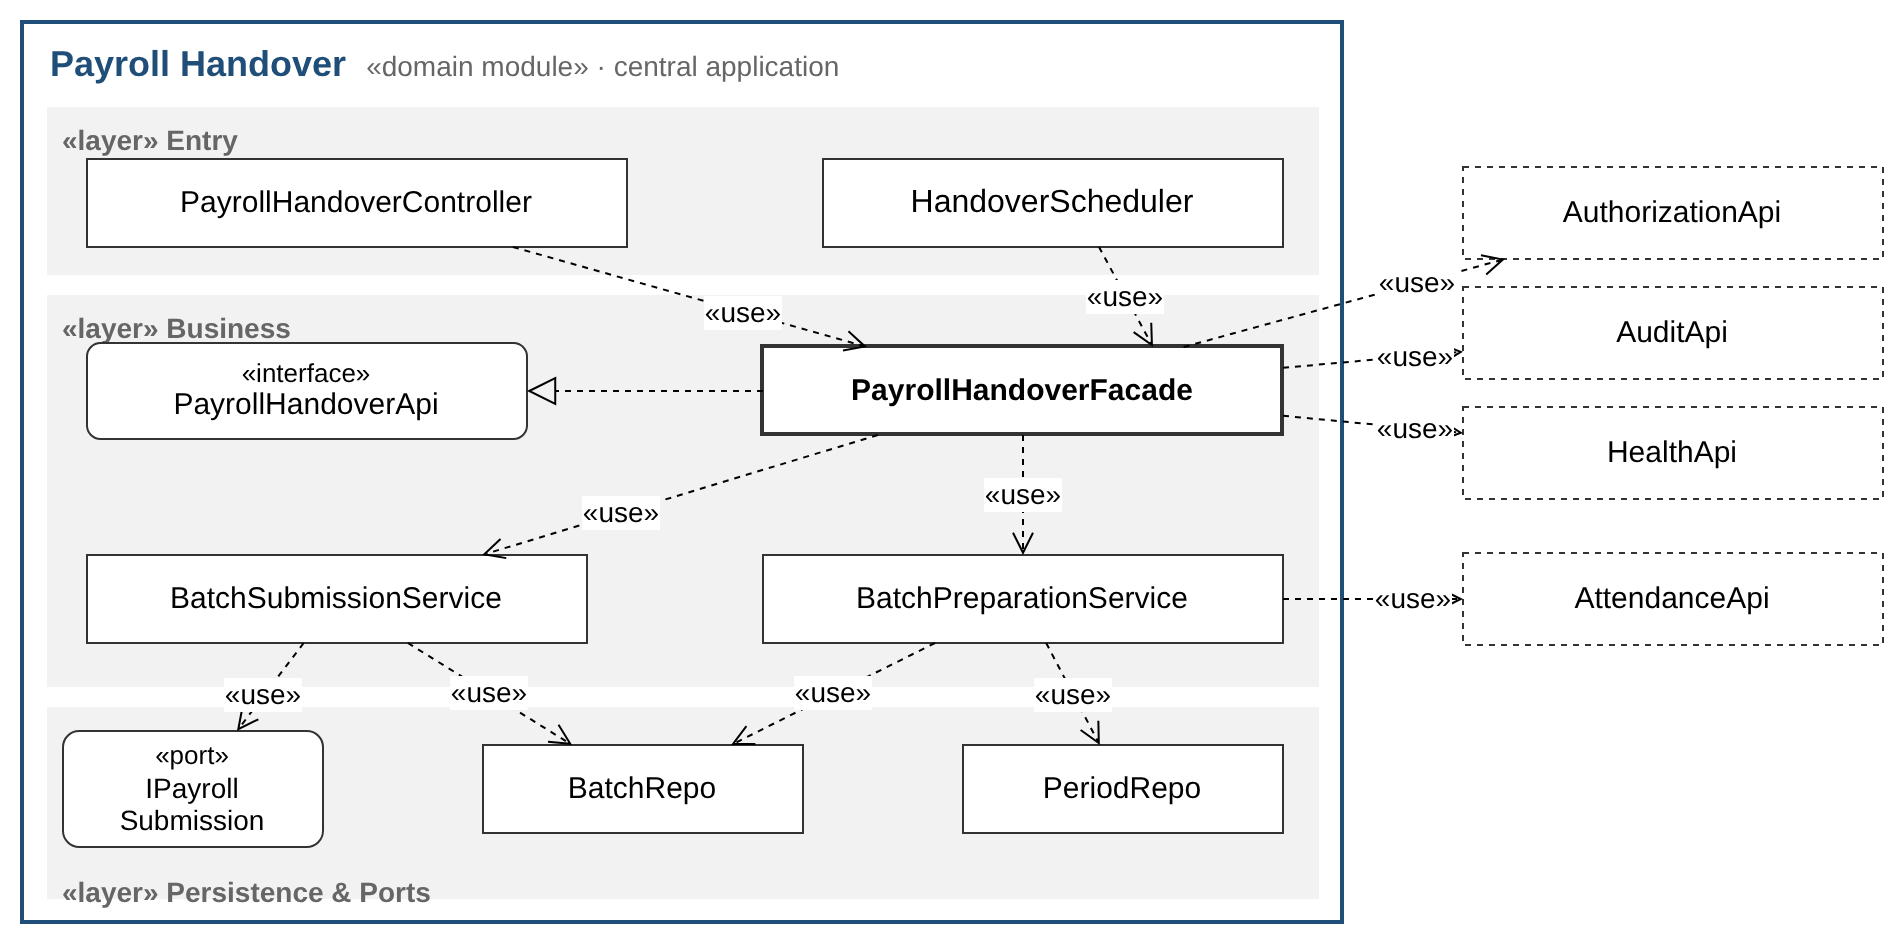
\includegraphics[width=450pt]{diagram/modules/figure-4-8-m7.png}

\vspace{6pt}
\textbf{Figure 4.8. M7 Payroll Handover}
\phantomsection\addcontentsline{lof}{figure}{\protect\numberline{4.8}M7 Payroll Handover}

\vspace{8pt}
{\small
\begin{tabular}{|>{\raggedright\arraybackslash}p{120pt}|>{\raggedright\arraybackslash}p{290pt}|}
\hline
\multicolumn{1}{|>{\columncolor{tableheader}\centering\arraybackslash}p{120pt}|}{\textbf{Component}} & \multicolumn{1}{>{\columncolor{tableheader}\centering\arraybackslash}p{290pt}|}{\textbf{Responsibility}} \\
\hline
Controller, HandoverScheduler & Accept manual actions and start the handover at 06:00 on day 1. \\
\hline
BatchPreparationService & Builds period and supplementary batches from attendance data. \\
\hline
BatchSubmissionService & Submits through IPayrollSubmission, queries the status where the API supports it, and stores CONFIRMED, REJECTED, or UNDETERMINED. \\
\hline
\end{tabular}
}

\vspace{6pt}
\textbf{Table 4.13. Components of M7 Payroll Handover}
\phantomsection\addcontentsline{lot}{table}{\protect\numberline{4.13}Components of M7 Payroll Handover}
\end{minipage}

\vspace{14pt}

\noindent\begin{minipage}{\linewidth}
Figure 4.9 shows the inside of HR/Payroll Integration, and Table 4.14 describes its components.

\vspace{6pt}
\centering
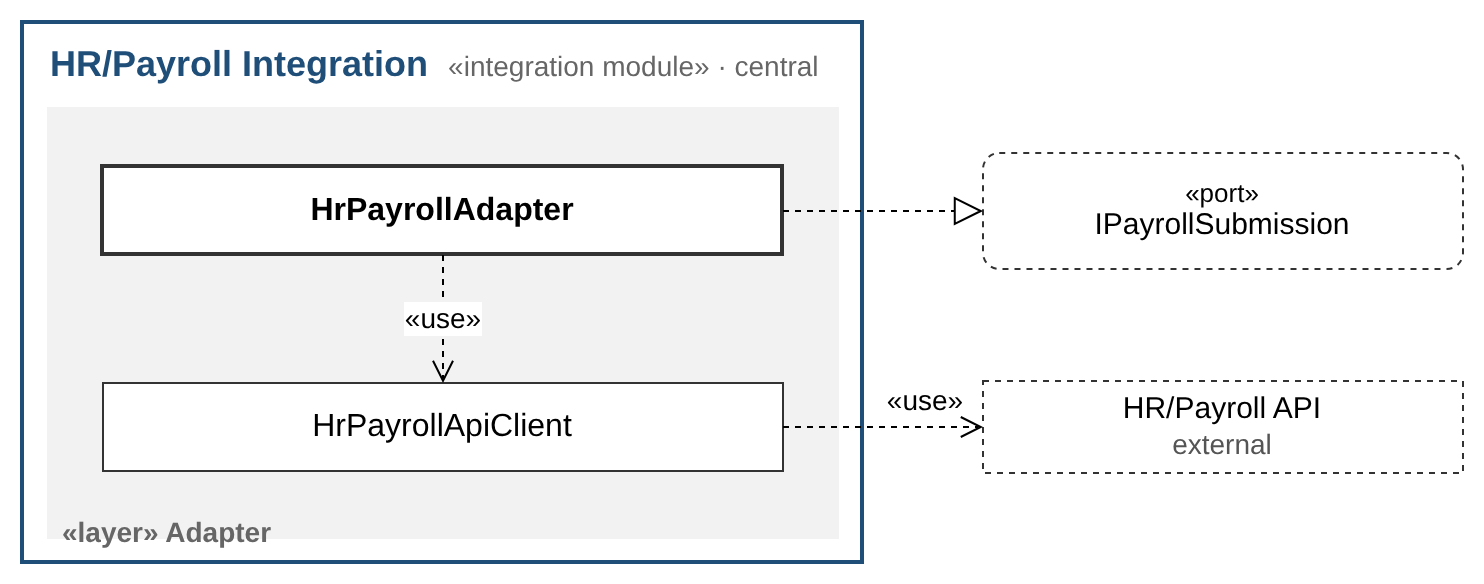
\includegraphics[width=350.3pt]{diagram/modules/figure-4-9-m8.png}

\vspace{6pt}
\textbf{Figure 4.9. M8 HR/Payroll Integration}
\phantomsection\addcontentsline{lof}{figure}{\protect\numberline{4.9}M8 HR/Payroll Integration}

\vspace{8pt}
{\small
\begin{tabular}{|>{\raggedright\arraybackslash}p{120pt}|>{\raggedright\arraybackslash}p{290pt}|}
\hline
\multicolumn{1}{|>{\columncolor{tableheader}\centering\arraybackslash}p{120pt}|}{\textbf{Component}} & \multicolumn{1}{>{\columncolor{tableheader}\centering\arraybackslash}p{290pt}|}{\textbf{Responsibility}} \\
\hline
HrPayrollAdapter & Implements IPayrollSubmission and translates batches and responses. \\
\hline
HrPayrollApiClient & Calls the HR/Payroll API and queries the status only if the API supports it (I-02). \\
\hline
\end{tabular}
}

\vspace{6pt}
\textbf{Table 4.14. Components of M8 HR/Payroll Integration}
\phantomsection\addcontentsline{lot}{table}{\protect\numberline{4.14}Components of M8 HR/Payroll Integration}
\end{minipage}

\vspace{14pt}

\noindent\begin{minipage}{\linewidth}
Figure 4.10 shows the inside of Site Sync, and Table 4.15 describes its components.

\vspace{6pt}
\centering
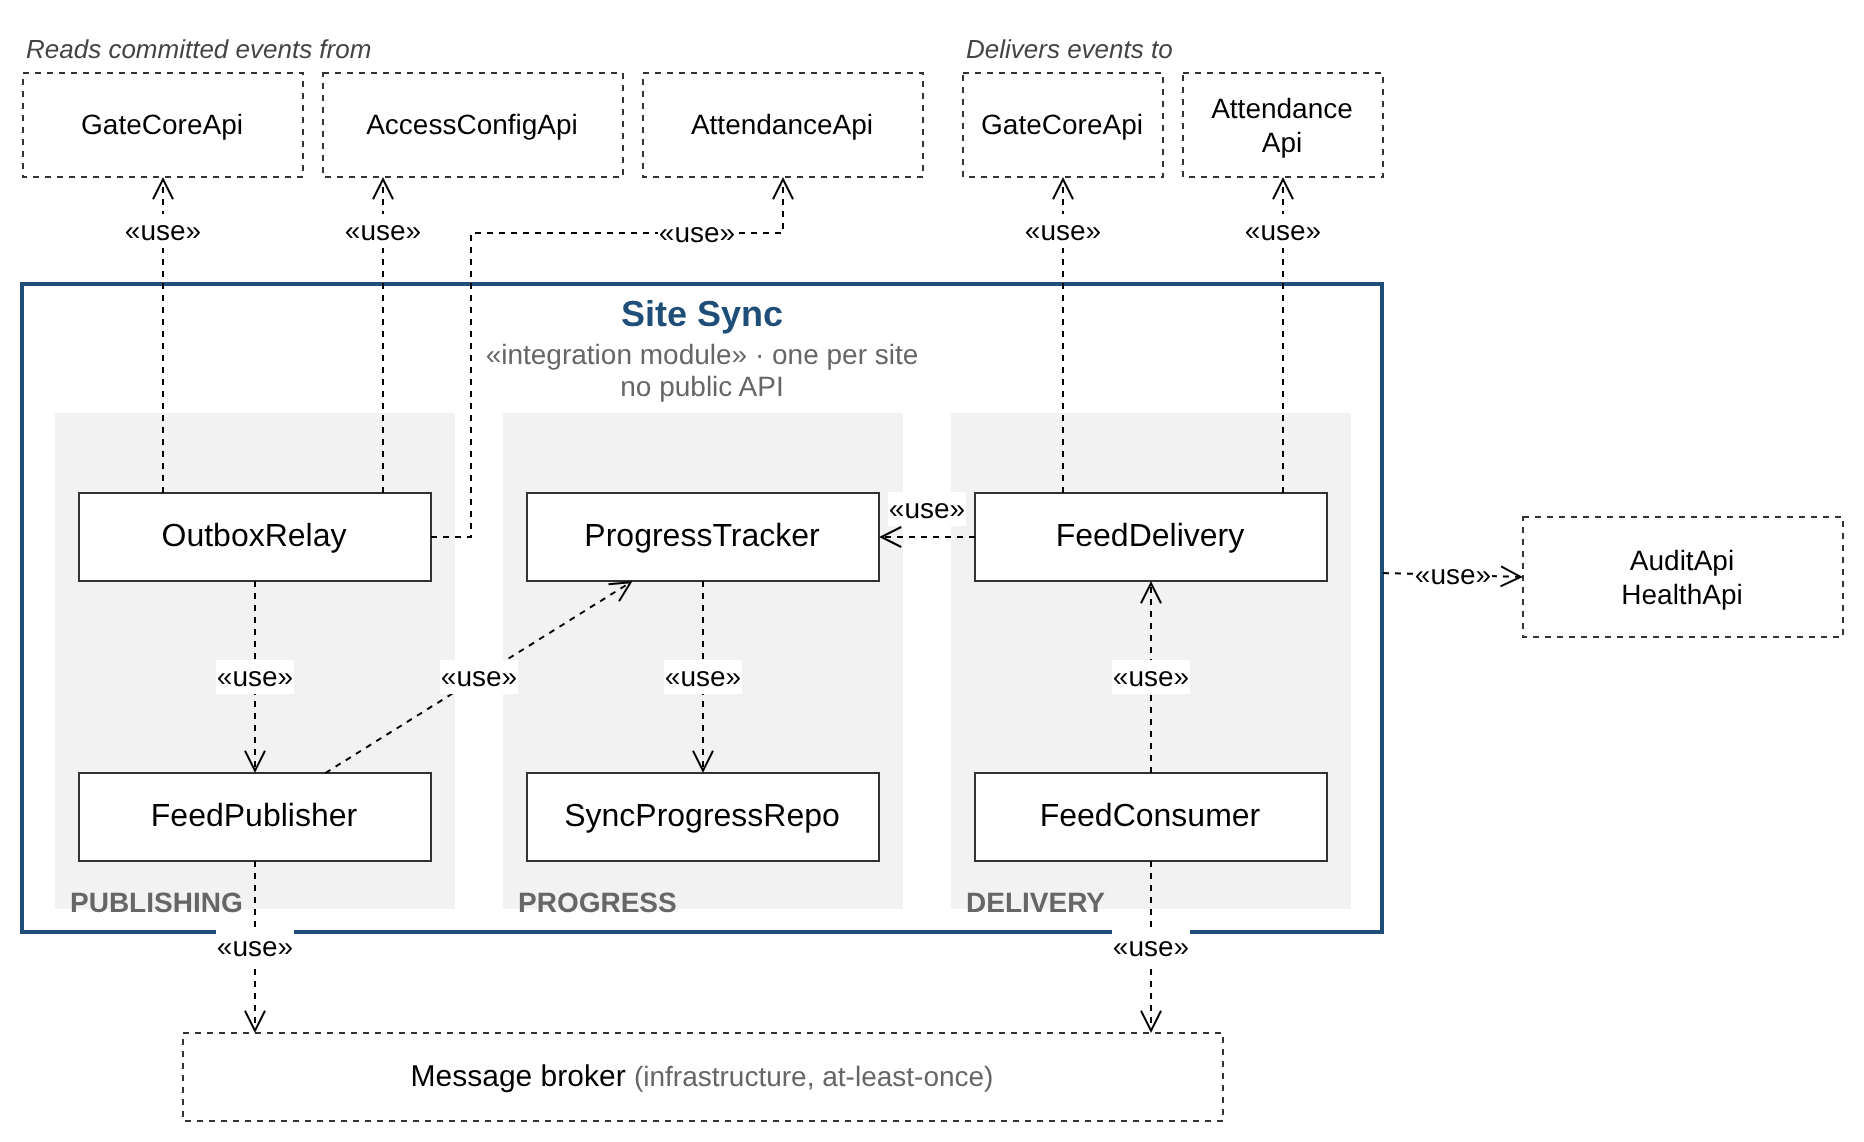
\includegraphics[width=440.5pt]{diagram/modules/figure-4-10-m9.png}

\vspace{6pt}
\textbf{Figure 4.10. M9 Site Sync}
\phantomsection\addcontentsline{lof}{figure}{\protect\numberline{4.10}M9 Site Sync}

\vspace{8pt}
{\small
\begin{tabular}{|>{\raggedright\arraybackslash}p{120pt}|>{\raggedright\arraybackslash}p{290pt}|}
\hline
\multicolumn{1}{|>{\columncolor{tableheader}\centering\arraybackslash}p{120pt}|}{\textbf{Component}} & \multicolumn{1}{>{\columncolor{tableheader}\centering\arraybackslash}p{290pt}|}{\textbf{Responsibility}} \\
\hline
OutboxRelay, FeedPublisher & Read committed events through the contracts of Gate Core, Access \& Configuration, and Attendance, and publish them with their original eventId. \\
\hline
FeedConsumer, FeedDelivery & Receive events from the broker and deliver them to Gate Core or Attendance; the acknowledgement is sent only after the receiver has stored the event. \\
\hline
ProgressTracker & Keeps watermarks and delivery progress and reports lag to Monitoring. \\
\hline
\end{tabular}
}

\vspace{6pt}
\textbf{Table 4.15. Components of M9 Site Sync}
\phantomsection\addcontentsline{lot}{table}{\protect\numberline{4.15}Components of M9 Site Sync}
\end{minipage}

\vspace{14pt}

\noindent\begin{minipage}{\linewidth}
Figure 4.11 shows the inside of Identity \& Access Control, and Table 4.16 describes its components.

\vspace{6pt}
\centering
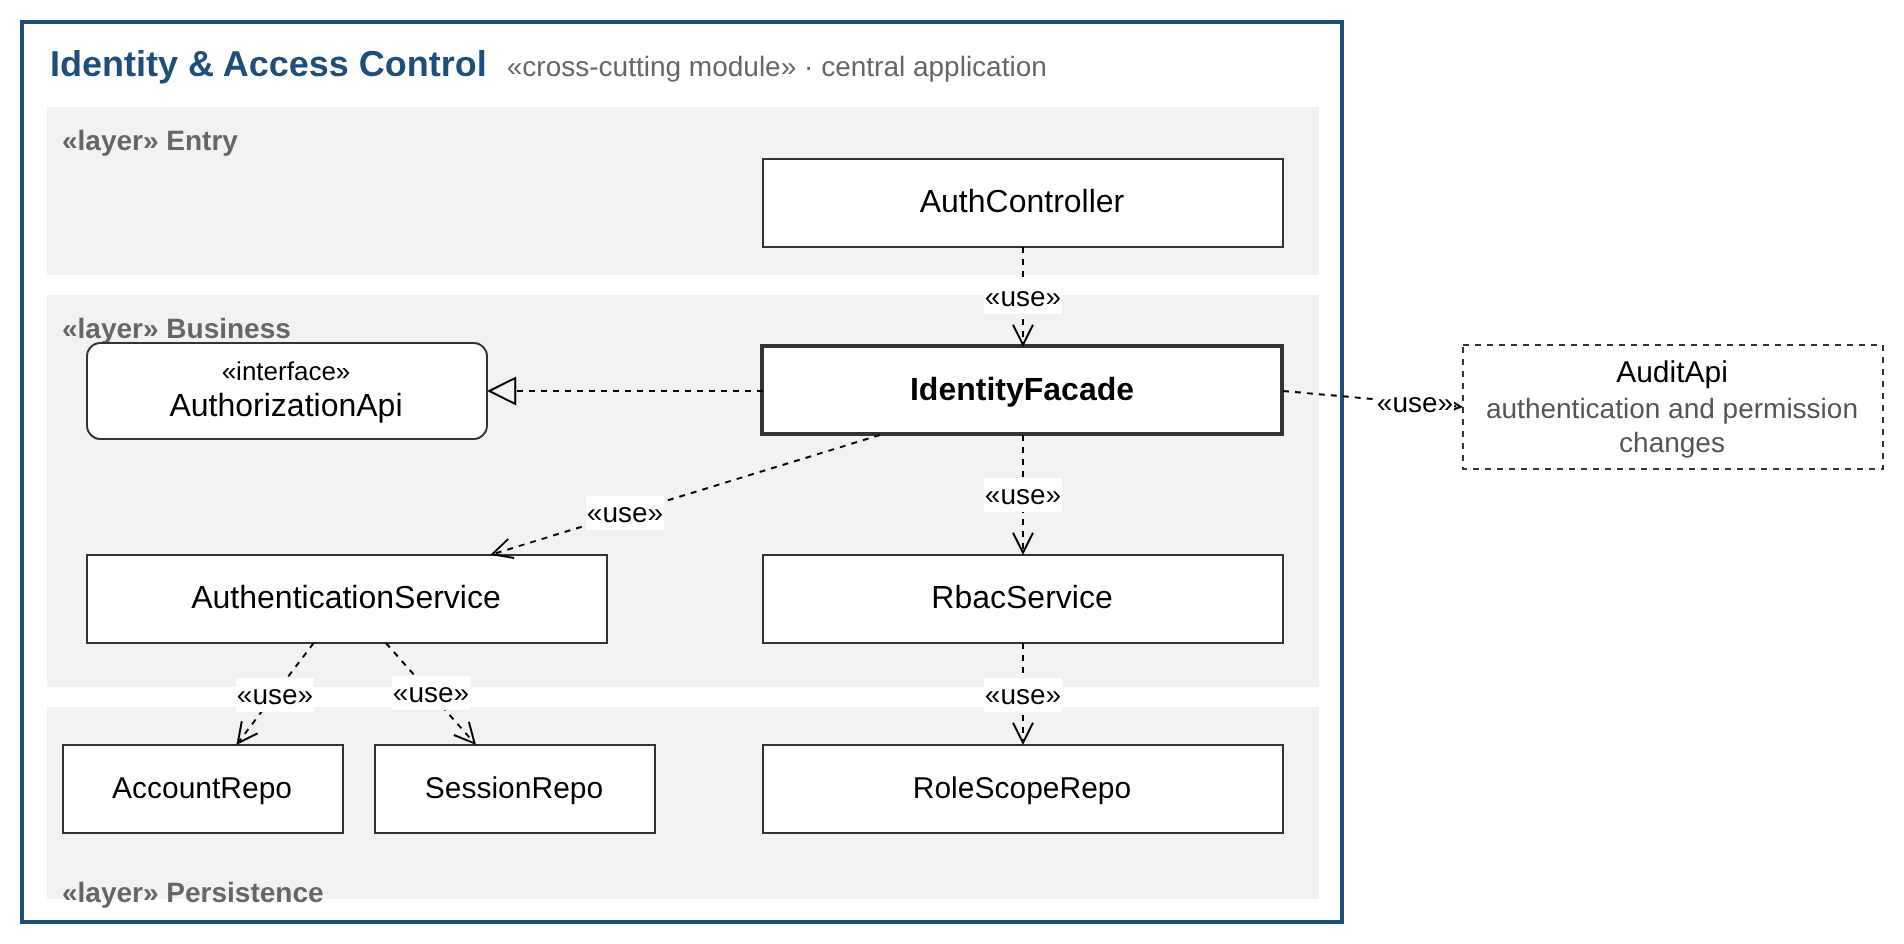
\includegraphics[width=450pt]{diagram/modules/figure-4-11-m10.png}

\vspace{6pt}
\textbf{Figure 4.11. M10 Identity \& Access Control}
\phantomsection\addcontentsline{lof}{figure}{\protect\numberline{4.11}M10 Identity \& Access Control}

\vspace{8pt}
{\small
\begin{tabular}{|>{\raggedright\arraybackslash}p{120pt}|>{\raggedright\arraybackslash}p{290pt}|}
\hline
\multicolumn{1}{|>{\columncolor{tableheader}\centering\arraybackslash}p{120pt}|}{\textbf{Component}} & \multicolumn{1}{>{\columncolor{tableheader}\centering\arraybackslash}p{290pt}|}{\textbf{Responsibility}} \\
\hline
AuthenticationService & Handles login and sessions. \\
\hline
RbacService & Manages roles and the action and data scope of each user. \\
\hline
IdentityFacade & Implements AuthorizationApi and sends authentication and permission-change evidence to Audit. \\
\hline
\end{tabular}
}

\vspace{6pt}
\textbf{Table 4.16. Components of M10 Identity \& Access Control}
\phantomsection\addcontentsline{lot}{table}{\protect\numberline{4.16}Components of M10 Identity \& Access Control}
\end{minipage}

\vspace{14pt}

\noindent\begin{minipage}{\linewidth}
Figure 4.12 shows the inside of Audit, and Table 4.17 describes its components.

\vspace{6pt}
\centering
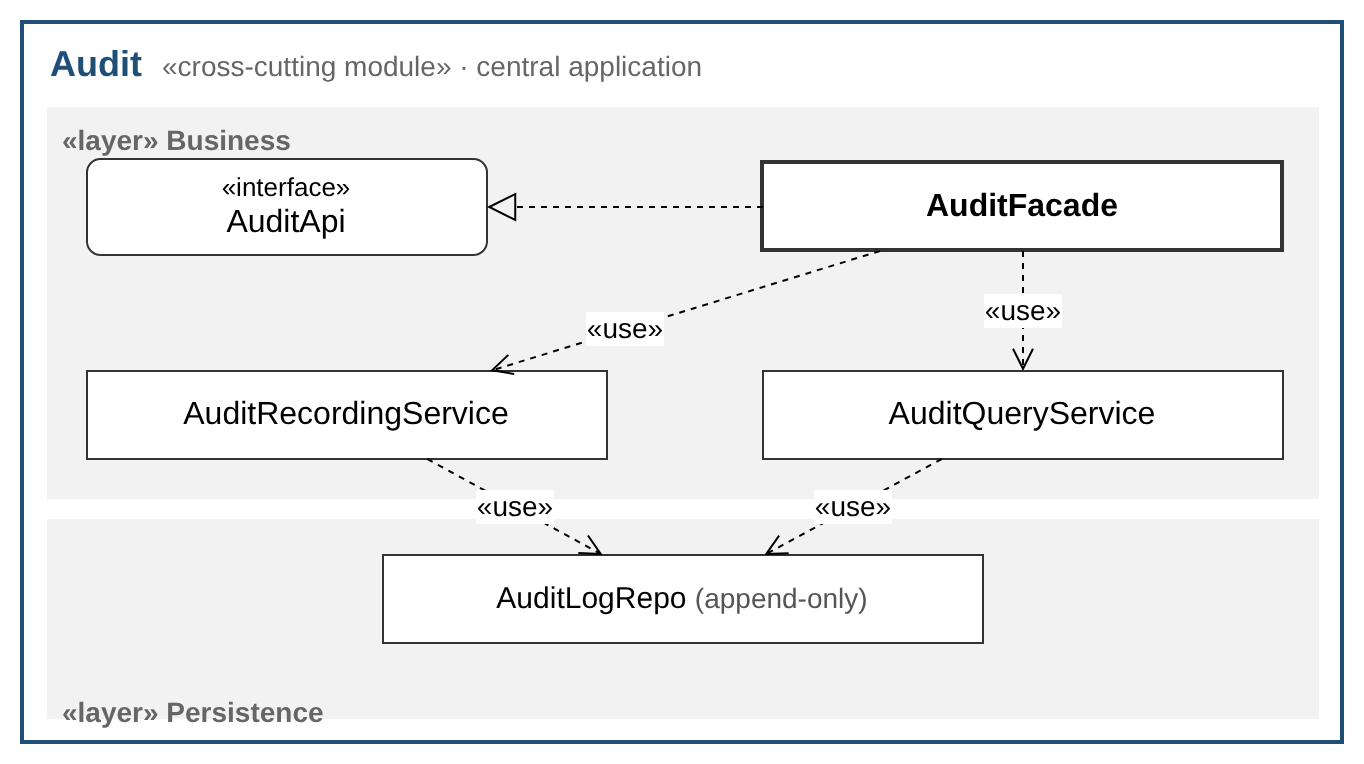
\includegraphics[width=321.8pt]{diagram/modules/figure-4-12-m11.png}

\vspace{6pt}
\textbf{Figure 4.12. M11 Audit}
\phantomsection\addcontentsline{lof}{figure}{\protect\numberline{4.12}M11 Audit}

\vspace{8pt}
{\small
\begin{tabular}{|>{\raggedright\arraybackslash}p{120pt}|>{\raggedright\arraybackslash}p{290pt}|}
\hline
\multicolumn{1}{|>{\columncolor{tableheader}\centering\arraybackslash}p{120pt}|}{\textbf{Component}} & \multicolumn{1}{>{\columncolor{tableheader}\centering\arraybackslash}p{290pt}|}{\textbf{Responsibility}} \\
\hline
AuditRecordingService & Appends audit records; existing records are never changed. \\
\hline
AuditQueryService & Answers queries that the caller has already scope-checked; Audit does not call Identity \& Access Control. \\
\hline
\end{tabular}
}

\vspace{6pt}
\textbf{Table 4.17. Components of M11 Audit}
\phantomsection\addcontentsline{lot}{table}{\protect\numberline{4.17}Components of M11 Audit}
\end{minipage}

\vspace{14pt}

\noindent\begin{minipage}{\linewidth}
Figure 4.13 shows the inside of Monitoring \& Operations, and Table 4.18 describes its components.

\vspace{6pt}
\centering
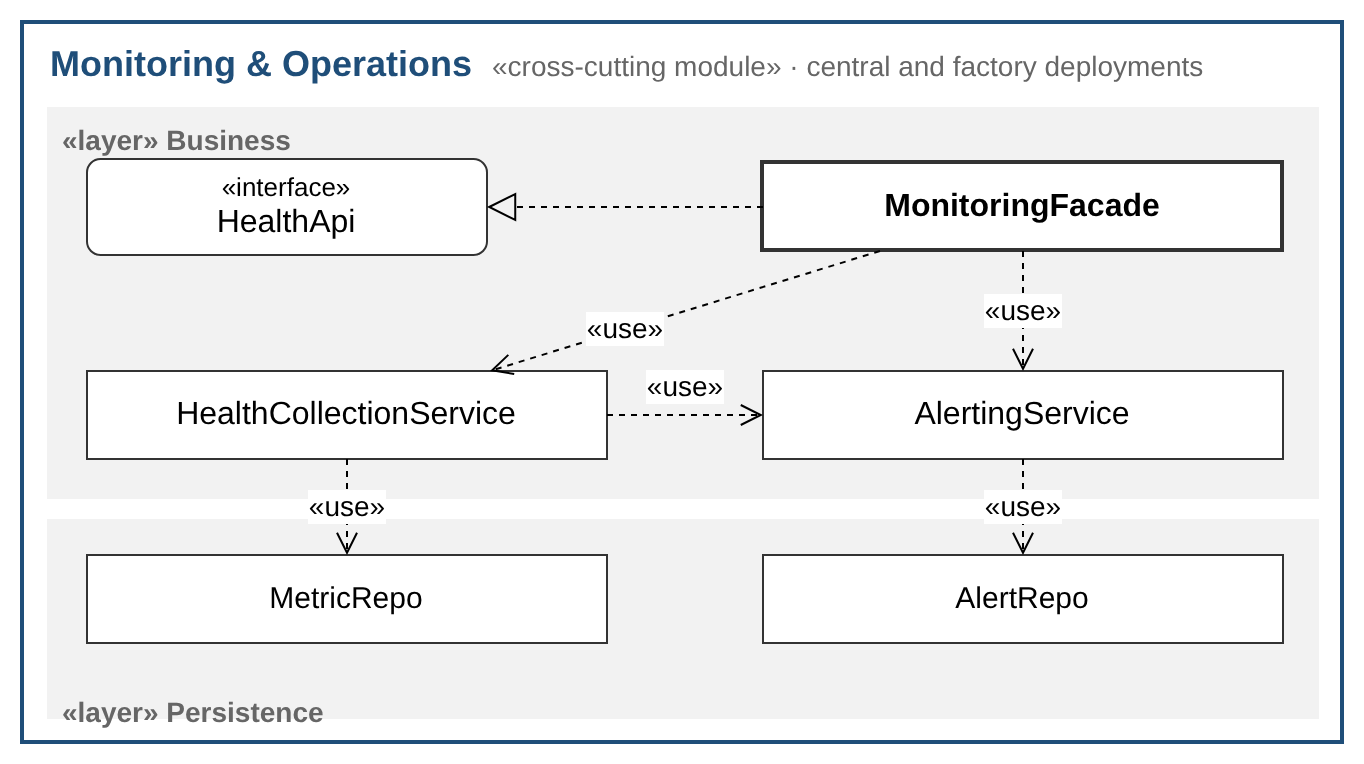
\includegraphics[width=321.8pt]{diagram/modules/figure-4-13-m12.png}

\vspace{6pt}
\textbf{Figure 4.13. M12 Monitoring \& Operations}
\phantomsection\addcontentsline{lof}{figure}{\protect\numberline{4.13}M12 Monitoring \& Operations}

\vspace{8pt}
{\small
\begin{tabular}{|>{\raggedright\arraybackslash}p{120pt}|>{\raggedright\arraybackslash}p{290pt}|}
\hline
\multicolumn{1}{|>{\columncolor{tableheader}\centering\arraybackslash}p{120pt}|}{\textbf{Component}} & \multicolumn{1}{>{\columncolor{tableheader}\centering\arraybackslash}p{290pt}|}{\textbf{Responsibility}} \\
\hline
MonitoringFacade & Implements HealthApi. It accepts reports from sources and returns the factory's current status and active alerts to Guard Status Display. \\
\hline
HealthCollectionService & Collects health, faults, latency, and progress. Sources report outside the scan response path, so Gate Core never waits for Monitoring. The factory deployment keeps working over the factory LAN when the WAN link is down and forwards its records to the central deployment when the link returns. \\
\hline
AlertingService & Raises alerts, for example on synchronization lag or a handover not confirmed by 10:00. \\
\hline
\end{tabular}
}

\vspace{6pt}
\textbf{Table 4.18. Components of M12 Monitoring \& Operations}
\phantomsection\addcontentsline{lot}{table}{\protect\numberline{4.18}Components of M12 Monitoring \& Operations}
\end{minipage}

\vspace{14pt}

\noindent\begin{minipage}{\linewidth}
Figure 4.14 shows the inside of Clients, and Table 4.19 describes its components.

\vspace{6pt}
\centering
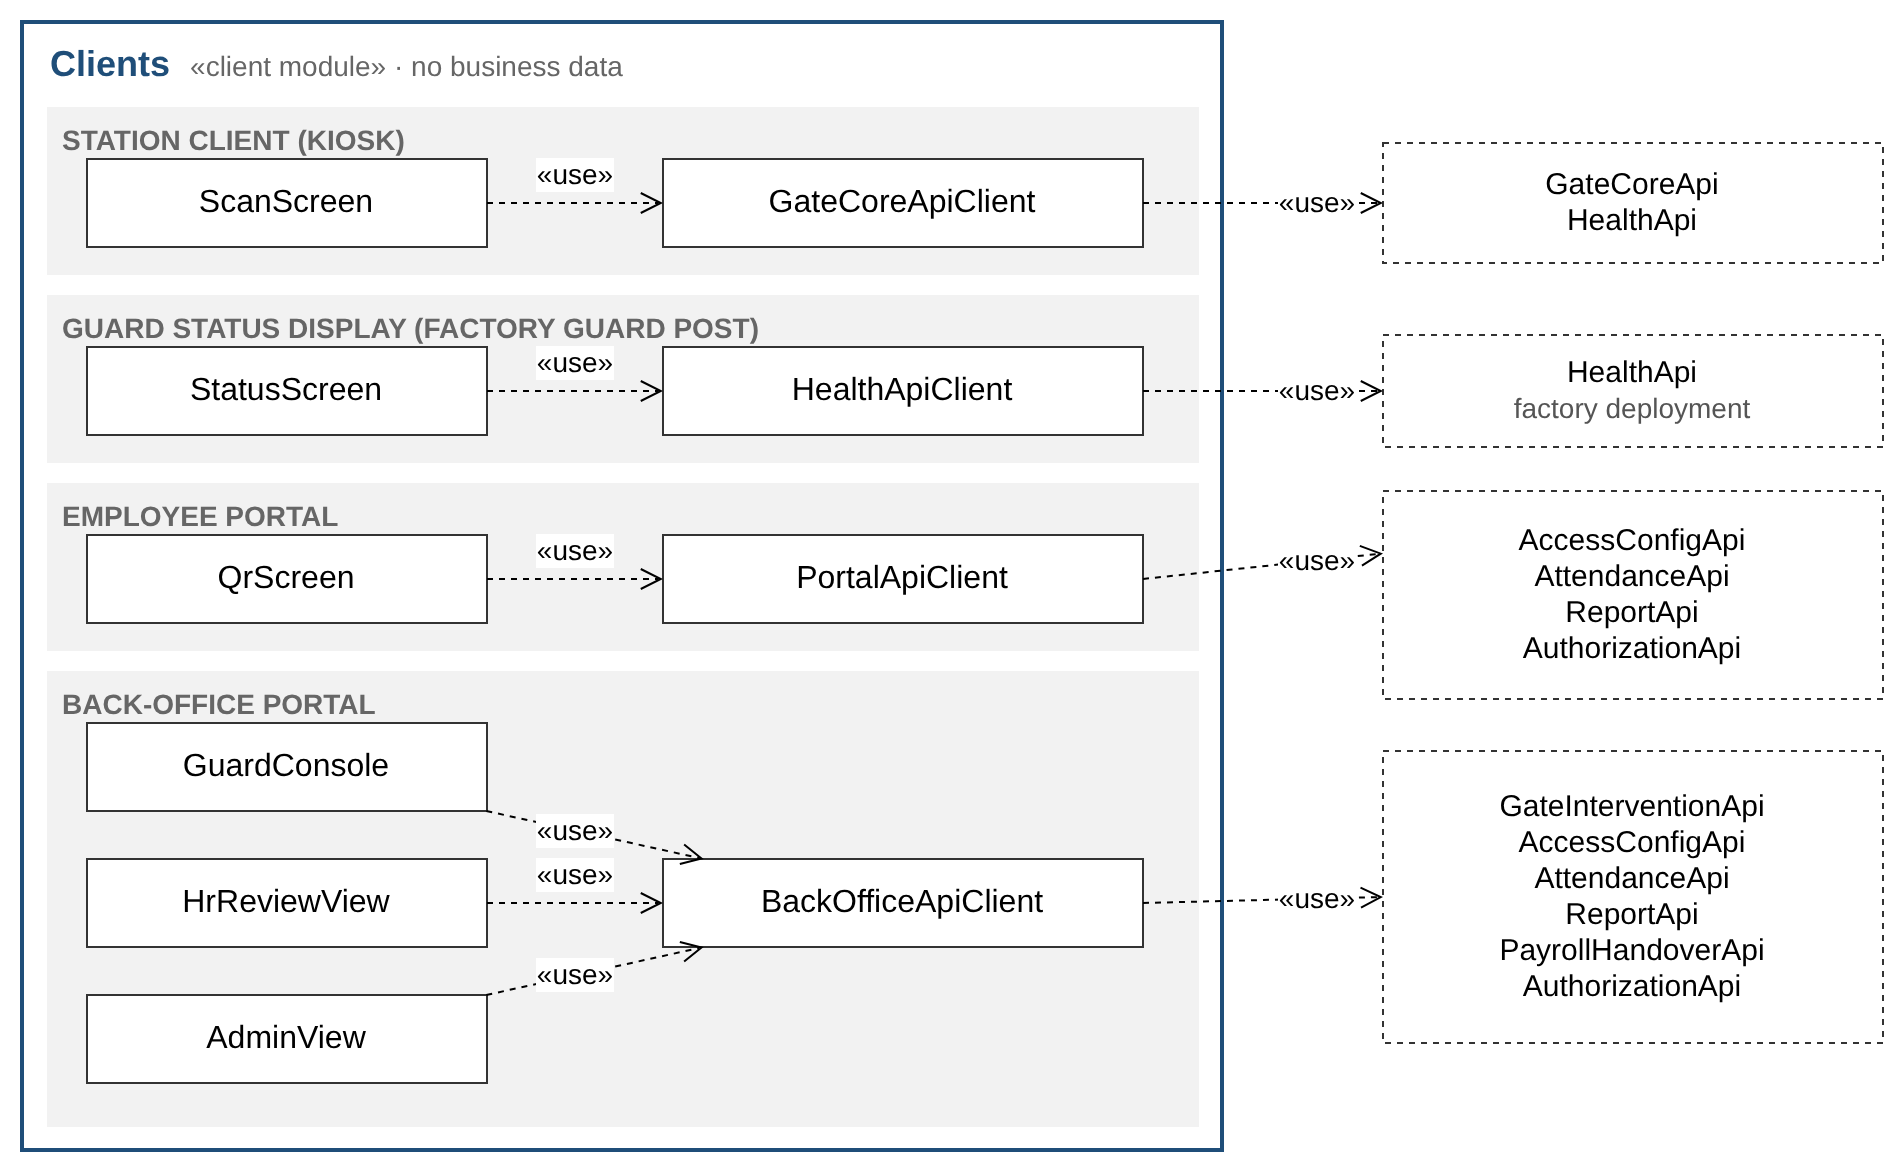
\includegraphics[width=450pt]{diagram/modules/figure-4-14-m13.png}

\vspace{6pt}
\textbf{Figure 4.14. M13 Clients}
\phantomsection\addcontentsline{lof}{figure}{\protect\numberline{4.14}M13 Clients}

\vspace{8pt}
{\small
\begin{tabular}{|>{\raggedright\arraybackslash}p{120pt}|>{\raggedright\arraybackslash}p{290pt}|}
\hline
\multicolumn{1}{|>{\columncolor{tableheader}\centering\arraybackslash}p{120pt}|}{\textbf{Component}} & \multicolumn{1}{>{\columncolor{tableheader}\centering\arraybackslash}p{290pt}|}{\textbf{Responsibility}} \\
\hline
Station Client & Shows the result, LANE BUSY, or UNDETERMINED, and calls getScanStatus with the same scanId after a timeout. \\
\hline
Employee Portal & Shows the QR screen and the employee's attendance history. \\
\hline
Back-office Portal & Provides the guard, HR, and administrator views. \\
\hline
Guard Status Display & A fixed screen at the factory guard post. It reads the factory's status and active alerts, such as degraded mode, from the factory deployment of Monitoring. It signs in with a device identity checked at the factory, so it works without central Identity \& RBAC, and it is read-only: assisted and emergency actions stay in Back-office Portal under the normal authorization rules. If it cannot reach the factory application, it shows that its data is stale. \\
\hline
\end{tabular}
}

\vspace{6pt}
\textbf{Table 4.19. Components of M13 Clients}
\phantomsection\addcontentsline{lot}{table}{\protect\numberline{4.19}Components of M13 Clients}
\end{minipage}

\vspace{14pt}

\subsection*{4.2. Component-and-Connector View}

\phantomsection
\addcontentsline{toc}{subsection}{4.2. Component-and-Connector View}

The C\&C View shows TMC at runtime: which components handle each request, which interfaces they call, and which connectors link the factory application, the central application, and the external systems. It consists of a component diagram, three runtime flows, and the states that keep these flows safe.

\subsubsection*{4.2.1. Component Diagram}

\phantomsection
\addcontentsline{toc}{subsubsection}{4.2.1. Component Diagram}

Figure 4.15 shows the runtime components of TMC and the connectors between them.

\noindent\begin{minipage}{\linewidth}
\centering
\IfFileExists{diagram/cc-view/figure-4-15-cc-view.png}{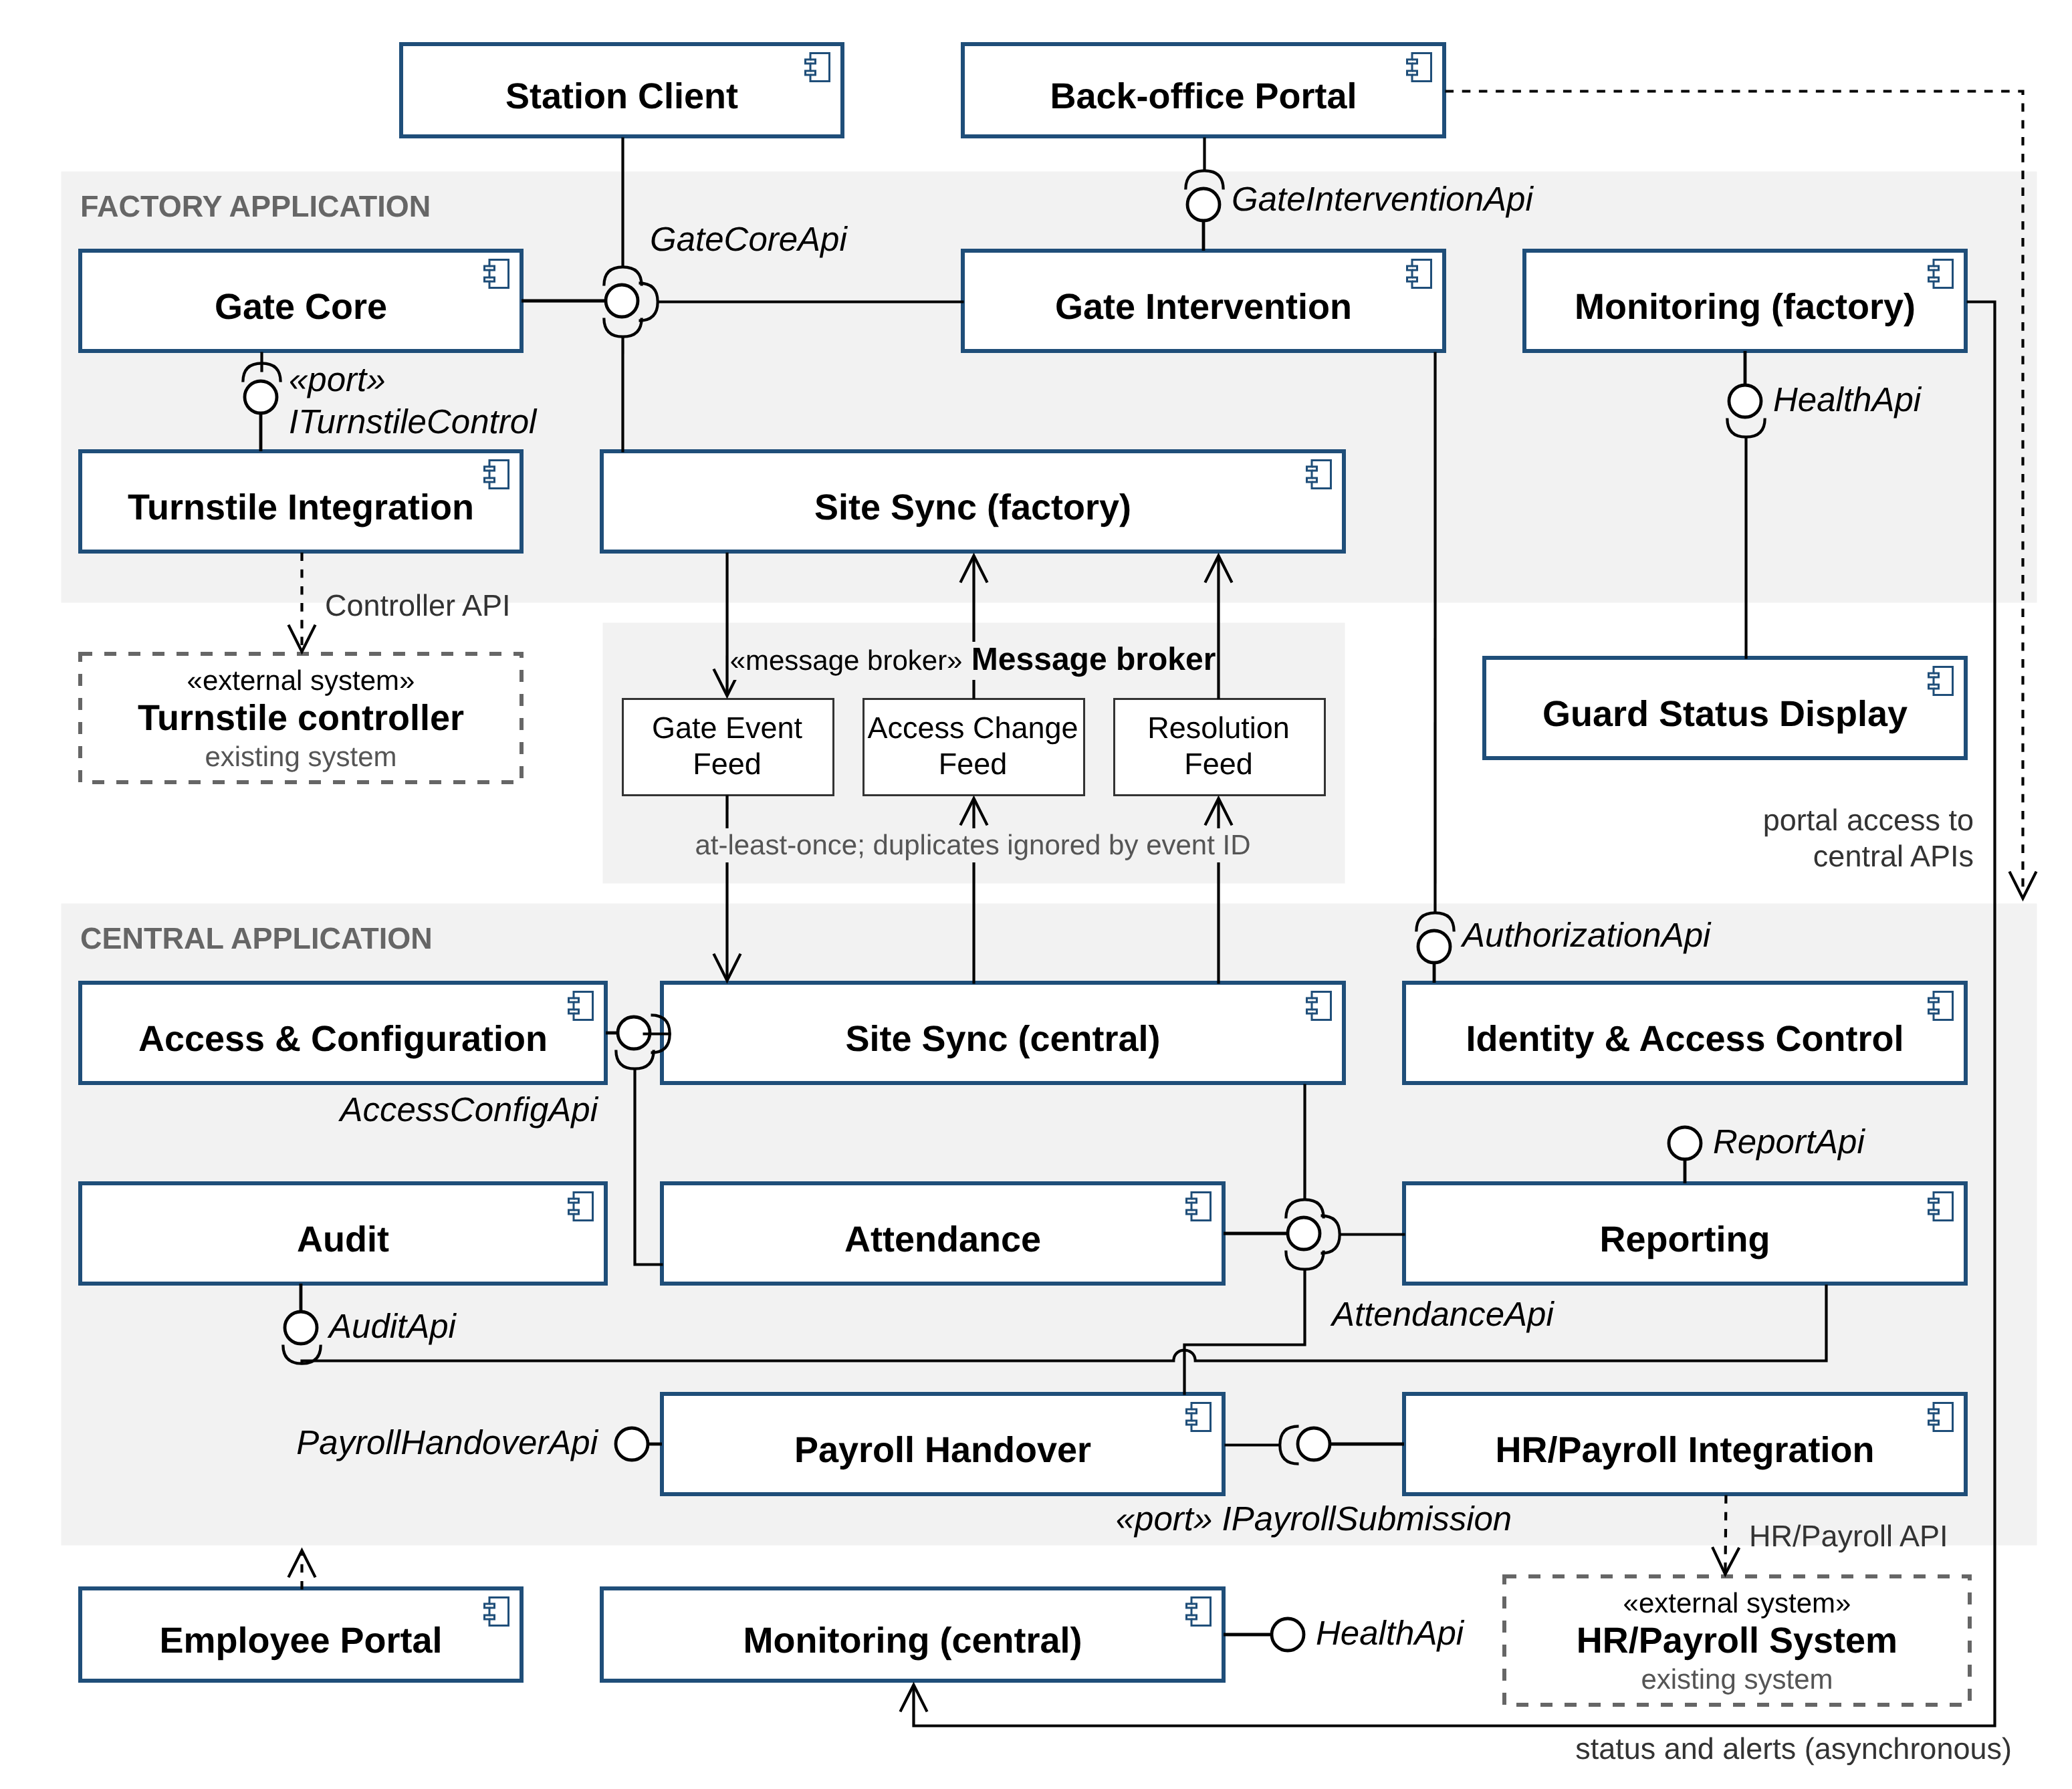
\includegraphics[width=450.0pt,height=620.0pt,keepaspectratio]{diagram/cc-view/figure-4-15-cc-view.png}}{\fbox{\parbox{300pt}{\centering\vspace{20pt}Figure being redrawn\vspace{20pt}}}}

\vspace{6pt}
\textbf{Figure 4.15. Component-and-Connector View of the TMC System}
\phantomsection\addcontentsline{lof}{figure}{\protect\numberline{4.15}Component-and-Connector View of the TMC System}
\end{minipage}

\medskip

\Needspace{6\baselineskip}
Figure 4.15 has five groups of elements:

\begin{itemize}[leftmargin=36pt, itemsep=2pt, topsep=4pt, parsep=2pt]
  \item \textbf{Clients:} Station Client on the kiosk sends scans through GateCoreApi. Employee Portal and Back-office Portal are separate clients for employees and staff. Guard Status Display on the guard screen reads the local HealthApi.
  \item \textbf{Factory application:} Gate Core, Turnstile Integration, Gate Intervention, the factory part of Site Sync, and factory Monitoring.
  \item \textbf{Central application:} Access \& Configuration, Attendance, Reporting, Payroll Handover, HR/Payroll Integration, Identity \& Access Control, Audit, and the central part of Site Sync. Central Monitoring runs outside both applications, on the monitoring server listed in Table 5.1.
  \item \textbf{Message broker:} carries three feeds with at-least-once delivery. Gate Event Feed takes scan events, transactions, assistance records, and ResolutionApplied from Gate Core to AttendanceApi. Access Change Feed takes versioned permissions, configuration, and verification keys from Access \& Configuration to Gate Core. Resolution Feed takes approved decisions linked to scans from Attendance Review to Gate Core.
  \item \textbf{External systems:} the turnstile controller, reached by Turnstile Adapter through the Controller API (I-01), and HR/Payroll, reached by HR/Payroll Adapter through the HR/Payroll API (I-02).
\end{itemize}

We draw the components in UML. Balls and half-circle sockets are provided and required interfaces, and a connected pair is a synchronous call. Solid open arrows are asynchronous transfers; factory Monitoring forwards status and alerts to central Monitoring separately from the broker. Dashed open arrows summarize portal access and external-system calls. To keep the figure readable, it leaves out the HealthApi reports and AuditApi appends of source components, the handover scheduler, Reporting's AccessConfigApi call, and TMC email integration.

\textbf{Interfaces and ports.} Table 4.20 lists the public APIs and integration contracts. The owner defines the contract. Turnstile Adapter implements the outgoing command ports, grouped as ITurnstileControl. Gate Core implements the separate incoming port IPassageEvents, which the adapter calls. Each API name stands for a group of operations, and a consumer only uses the ones it needs.

{\small
\begin{longtable}{|>{\raggedright\arraybackslash}p{92pt}|>{\raggedright\arraybackslash}p{68pt}|>{\raggedright\arraybackslash}p{132pt}|>{\raggedright\arraybackslash}p{105pt}|}
\hline
\multicolumn{1}{|>{\columncolor{tableheader}\centering\arraybackslash}p{92pt}|}{\textbf{API or port}} & \multicolumn{1}{>{\columncolor{tableheader}\centering\arraybackslash}p{68pt}|}{\textbf{Owner}} & \multicolumn{1}{>{\columncolor{tableheader}\centering\arraybackslash}p{132pt}|}{\textbf{Main operations}} & \multicolumn{1}{>{\columncolor{tableheader}\centering\arraybackslash}p{105pt}|}{\textbf{Consumers}} \\
\hline
\endhead
\multicolumn{4}{c}{\rule{0pt}{22pt}\normalsize\textbf{Table 4.20. Public Interfaces and Integration Ports}} \\
\endlastfoot
GateCoreApi & Gate Core (M1) & submitScan, getScanStatus; recordIntervention, requestAssistedOpen, requestEmergencyRelease, requestEmergencyReset; applyEligibilityChanges, applyScanResolution; read committed Gate Event Feed events & Station Client; Gate Intervention; Site Sync \\
\hline
GateInterventionApi & Gate Intervention (M3) & recordAssistedAccess, authorizeAssistedOpen, emergencyRelease, resetEmergency & Back-office Portal \\
\hline
AccessConfigApi & Access \& Configuration (M4) & issue fresh QR; request email display link; manage rights, stations, shifts, and rules; read committed Access Change Feed events & Employee Portal; Back-office Portal; Attendance; Reporting; Site Sync \\
\hline
AttendanceApi & Attendance (M5) & receive events; review and approve cases; query period data and open cases; read committed Resolution Feed events & Site Sync; Employee Portal; Back-office Portal; Reporting; Payroll Handover \\
\hline
ReportApi & Reporting (M6) & query attendance, reports, and authorized audit data & Employee Portal; Back-office Portal \\
\hline
PayrollHandoverApi & Payroll Handover (M7) & start period, query progress, prepare supplementary handover & Scheduler; Back-office Portal \\
\hline
AuthorizationApi & Identity \& Access Control (M10) & check identity, action, and data scope; administer accounts separately & Business components; Employee Portal; Back-office Portal \\
\hline
AuditApi & Audit (M11) & append source evidence; query authorized history & Source components; Reporting \\
\hline
HealthApi & Monitoring \& Operations (M12) & report health, faults, latency, and progress; read the factory's current status and active alerts & Report: Station Client; Gate Core; Turnstile Integration; Site Sync; Payroll Handover. Read: Guard Status Display \\
\hline
Turnstile ports & Gate Core (M1) & ITurnstileControl groups openGate (IOpenGate), closeGate (ICloseGate), and emergencyRelease/resetEmergency (IEmergencyGate), all returning results. IPassageEvents carries PASSAGE and LANE\_CLEAR. Status query is optional. & M2 implements command ports; M1 uses them. M1 implements IPassageEvents; M2 calls it \\
\hline
IPayrollSubmission & Payroll Handover (M7) & submit batch, receive outcome, inquire where supported & Payroll Handover uses; implemented by HR/Payroll Integration (M8) \\
\hline
\end{longtable}
}
\phantomsection\addcontentsline{lot}{table}{\protect\numberline{4.20}Public Interfaces and Integration Ports}

\Needspace{6\baselineskip}
Three rules apply across these interfaces:

\begin{itemize}[leftmargin=36pt, itemsep=2pt, topsep=4pt, parsep=2pt]
  \item \textbf{Permissions per operation.} Using an API group does not give a consumer every operation in it; authorization is checked where the request is processed. Station Client can submit and query scans but cannot call recordIntervention, and Employee Portal cannot approve cases.
  \item \textbf{Events through contracts.} Site Sync reads committed events through source-owned contracts and keeps their event IDs and versions; it never reads module repositories. Receivers use event IDs, object IDs, and versions to ignore duplicates and to spot missing or out-of-order data.
  \item \textbf{Internal calls stay internal.} Calls inside one module, such as Gate Transaction Processor to Access Decision or Attendance Review to Attendance Consolidation, are not public interfaces and are not listed in Table 4.20.
\end{itemize}

\Needspace{6\baselineskip}
\textbf{Data ownership.} Each kind of data has one owner, and other modules reach it only through that owner's interface:

\begin{itemize}[leftmargin=36pt, itemsep=2pt, topsep=4pt, parsep=2pt]
  \item Gate Core: scan states, transactions originating at gates, assistance records received at their source, and Eligibility Snapshot.
  \item Access \& Configuration: employee information, factory access permissions, station and lane configuration, shift schedules, and aggregation rules.
  \item Attendance: consolidated attendance data, review records, and decisions. Attendance Consolidation updates attendance outcomes; Attendance Review manages cases and approvals.
  \item Payroll Handover: handover periods, batch content, and acknowledgement evidence.
  \item Audit: audit data received from sources.
  \item Identity \& Access Control: accounts, roles, system access permissions, and login sessions.
  \item Monitoring \& Operations: monitoring information, faults, alerts, and operational task progress.
\end{itemize}

Gate Intervention never writes Gate Core's data directly; it asks Gate Core through recordIntervention and the assisted and emergency requests.

\textbf{External contracts.} For the controller, we use the results and events assumed in I-01 and I-05. Each of OPEN\_CONFIRMED, PASSAGE, LANE\_CLEAR, and CLOSED is reported for a given lane and command. OPEN\_CONFIRMED and CLOSED come back as command results, while PASSAGE and LANE\_CLEAR arrive later as separate events. Gate Core sends closeGate once after LANE\_CLEAR, and the controller's own interlock must still prevent unsafe closing. After an emergency release, closing also needs an authorized reset and confirmation that release mode has ended. If any of these confirmations is missing, Gate Core alerts the guard and leaves recovery to the approved safety procedure. Email Link Sender sends only a link through TMC's email service, never a QR image, and the employee signs in before seeing a fresh code (I-08); an email failure does not affect the app or the web portal. Signals, status inquiry, acknowledgement, and duplicate handling must all be checked against the real APIs.

\noindent\begin{minipage}{\linewidth}
Table 4.21 summarizes the connector types.

\vspace{8pt}
\centering
\begin{tabular}{|>{\raggedright\arraybackslash}p{83.5pt}|>{\raggedright\arraybackslash}p{155.5pt}|>{\raggedright\arraybackslash}p{170.5pt}|}
\hline
\multicolumn{1}{|>{\columncolor{tableheader}\centering\arraybackslash}p{83.5pt}|}{\textbf{Type}} & \multicolumn{1}{>{\columncolor{tableheader}\centering\arraybackslash}p{155.5pt}|}{\textbf{Used In}} & \multicolumn{1}{>{\columncolor{tableheader}\centering\arraybackslash}p{170.5pt}|}{\textbf{Meaning}} \\
\hline
Synchronous call & Clients to interfaces; components to functions requiring results; internal module calls & The caller waits for the result before continuing. \\
\hline
Asynchronous event channel & Gate Event Feed; Access Change Feed; Resolution Feed; audit and operational information transfer & Recipients process at their own pace, with appropriate acknowledgements and duplicate prevention. \\
\hline
Port implementation & Turnstile Adapter with the turnstile command ports; Gate Core with IPassageEvents; HR/Payroll Adapter with IPayrollSubmission & A contract relationship between an adapter and the module defining the port; not a business message. \\
\hline
External system call & Adapters to the controller or HR/Payroll & Subject to external API conditions for timeouts, responses, inquiries, and resubmissions. \\
\hline
\end{tabular}

\vspace{6pt}
\textbf{Table 4.21. Connector Types}
\phantomsection\addcontentsline{lot}{table}{\protect\numberline{4.21}Connector Types}
\end{minipage}

\medskip

\Needspace{6\baselineskip}
Four points of the design are visible in Figure 4.15:

\begin{itemize}[leftmargin=36pt, itemsep=2pt, topsep=4pt, parsep=2pt]
  \item \textbf{Short synchronous path.} Only Station Client, Gate Core, and Turnstile Adapter are on the path the kiosk waits for, and all of them are in the factory. Reporting, handover, and synchronization are outside this response path; shared-resource contention still needs limits and performance tests (AC-03). Once the confirmed opening is stored, passage recording and safe closure run independently of the kiosk result.
  \item \textbf{Events between sites.} Business data between a factory and the central site moves only through the three feeds, so a WAN outage delays this data instead of stopping the QR flow, within the limits of I-10 (AC-01, AC-02). The exception is assisted and emergency opening, which waits synchronously for Identity \& RBAC at the central site (Table 3.2).
  \item \textbf{One adapter per external system.} The controller and HR/Payroll are each reached through one adapter, so an API change stays inside that adapter (AC-06).
  \item \textbf{Audit at the source.} Each source records audit evidence before sending it asynchronously to Audit Log, and Reporting checks authorization before calling AuditApi.query (AC-05). Chapter 7 covers what is audited and how long it is kept.
\end{itemize}

\clearpage
\subsubsection*{4.2.2. Flow A: QR Scan, Opening, Passage and Closure}

\phantomsection
\addcontentsline{toc}{subsubsection}{4.2.2. Flow A: QR Scan, Opening, Passage and Closure}

Figure 4.16 shows the gate flow for one scan, from the kiosk to the safe closure of the lane. The 2-second target of NFR-01 ends when the kiosk displays the result.

\noindent\begin{minipage}{\linewidth}
\centering
\IfFileExists{diagram/sequence/figure-4-16-qr-scan.png}{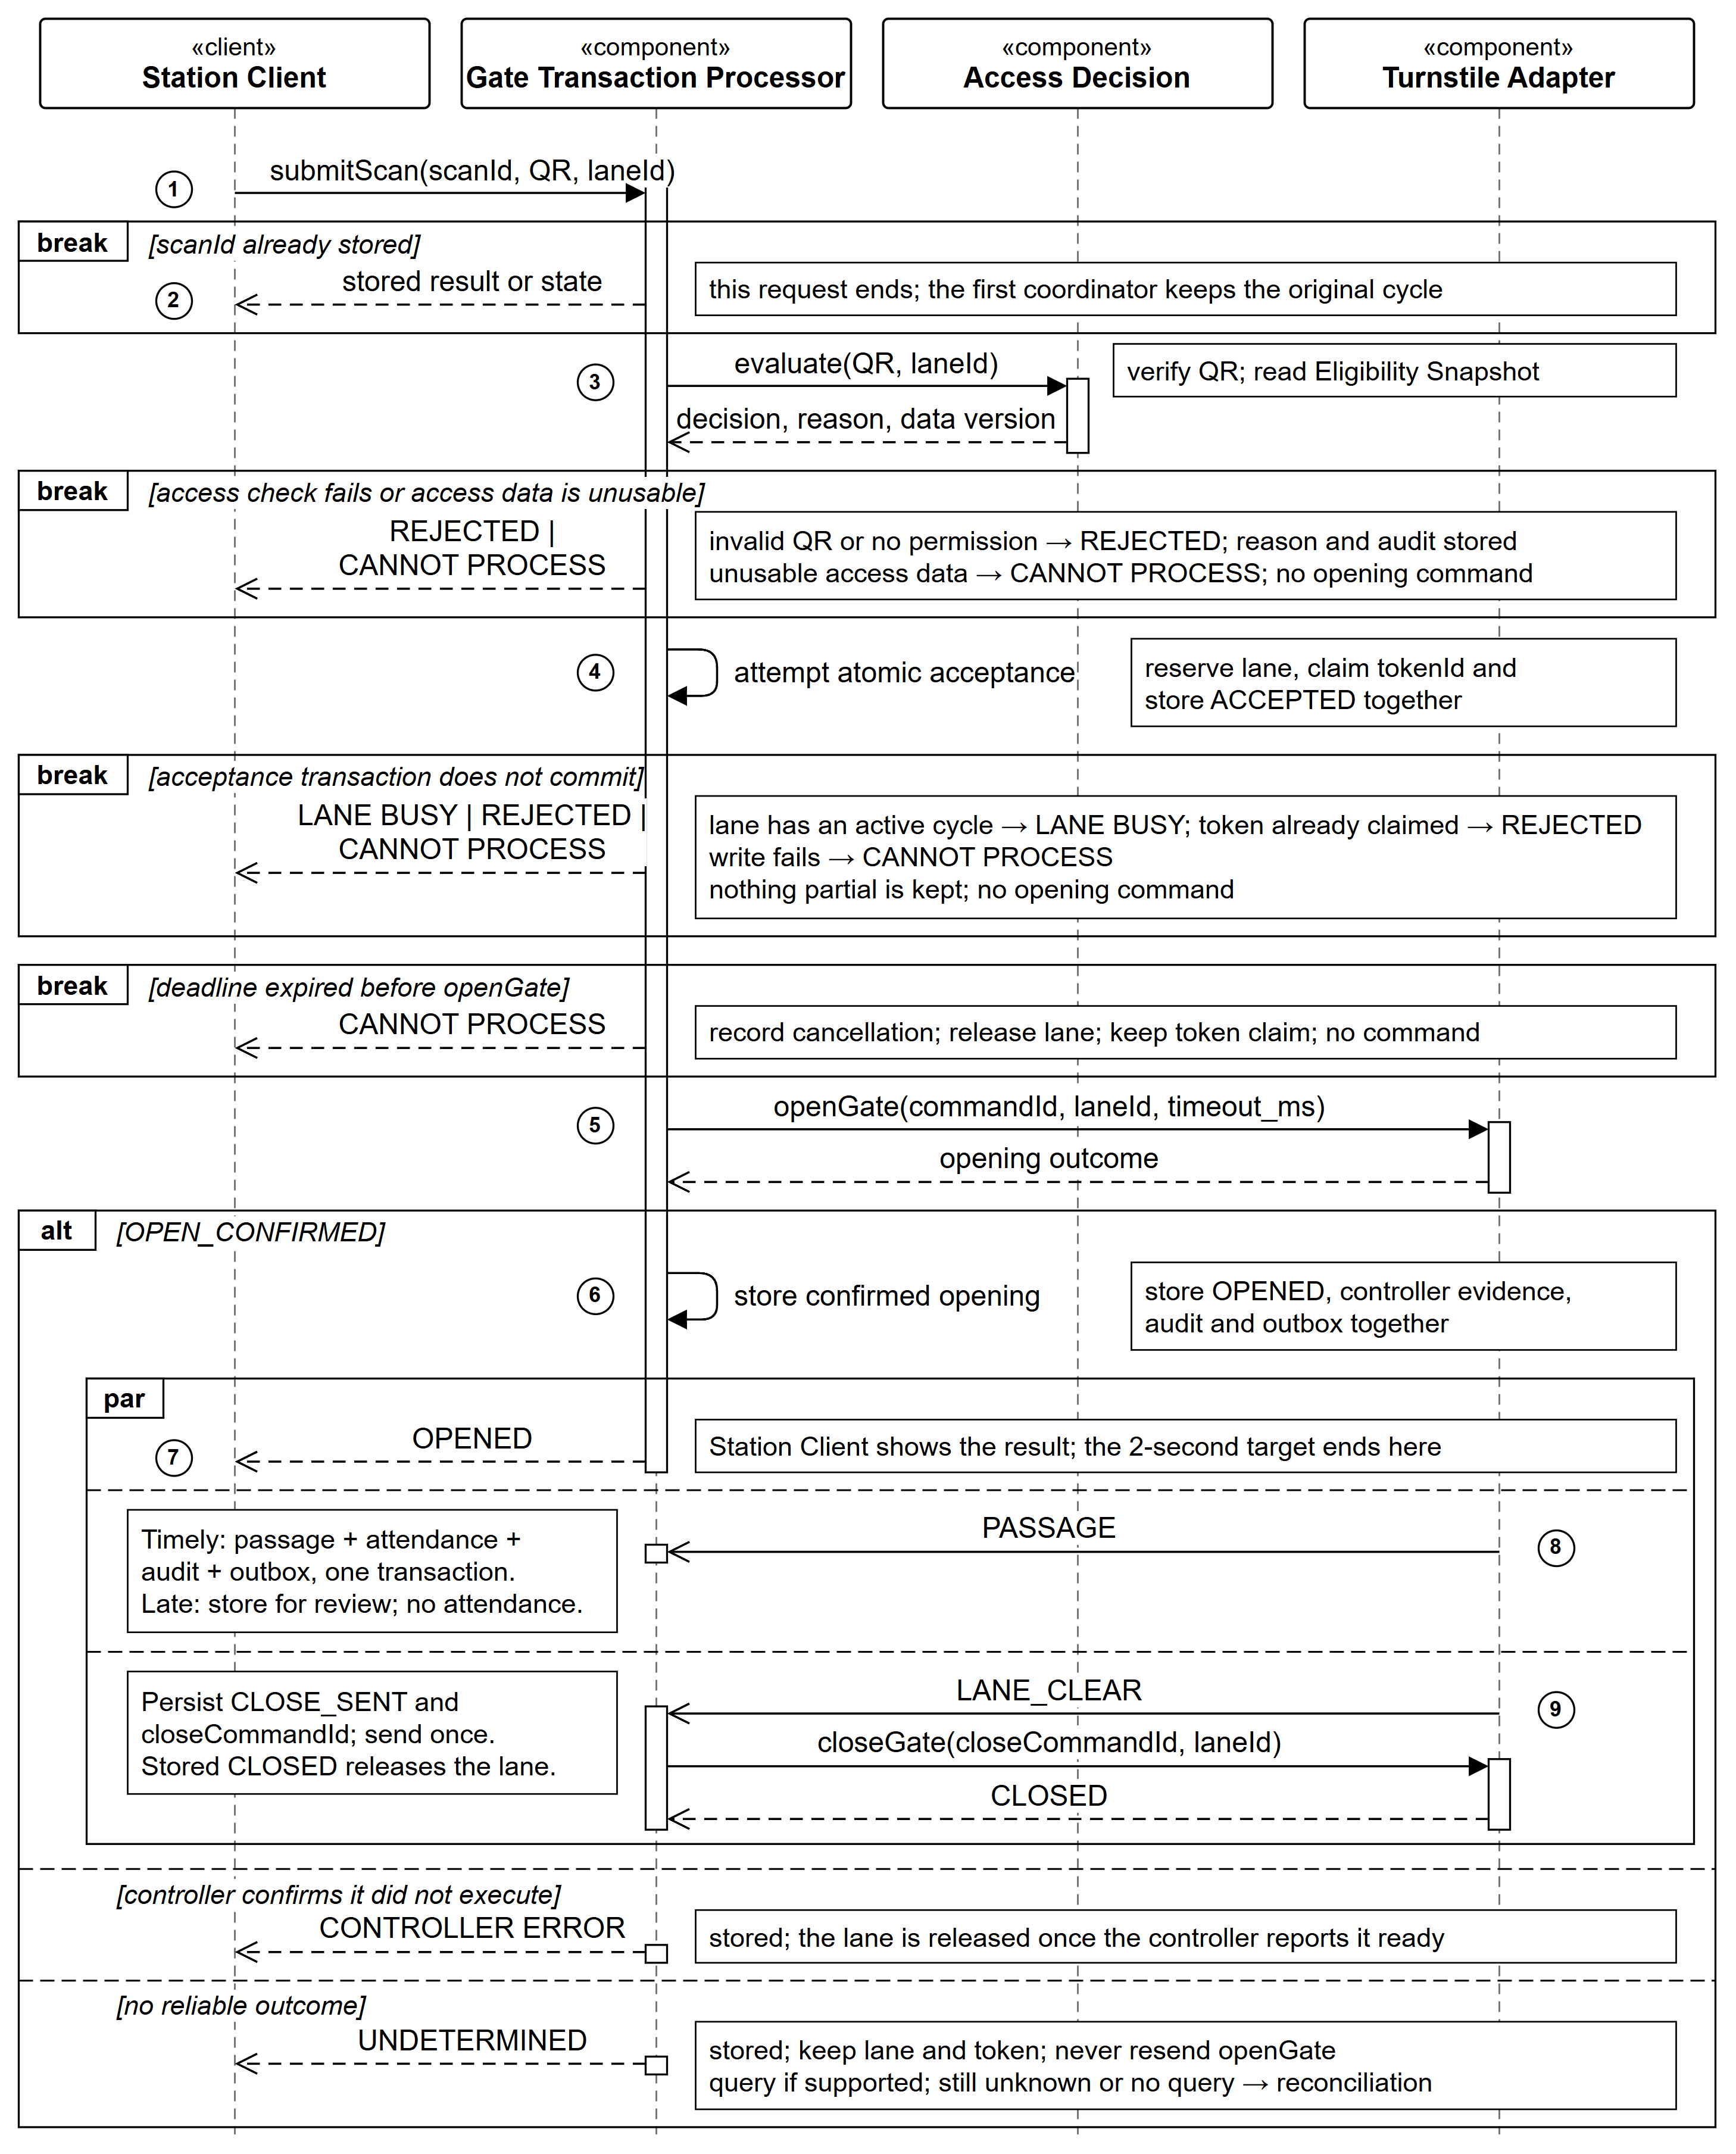
\includegraphics[width=450.0pt,height=555.0pt,keepaspectratio]{diagram/sequence/figure-4-16-qr-scan.png}}{\fbox{\parbox{300pt}{\centering\vspace{20pt}Figure being redrawn\vspace{20pt}}}}

\vspace{6pt}
\textbf{Figure 4.16. QR Scan Sequence --- Validation, Opening, Passage and Closure}
\phantomsection\addcontentsline{lof}{figure}{\protect\numberline{4.16}QR Scan Sequence --- Validation, Opening, Passage and Closure}
\end{minipage}

\vspace{8pt}

\Needspace{6\baselineskip}
Solid arrows with filled heads are synchronous calls, solid open arrows are signals, and dashed open arrows are returns; PASSAGE and LANE\_CLEAR come from the controller through Turnstile Adapter as events, and CLOSED comes back as the result of closeGate. Four break fragments stop the flow on a duplicate request, a failed check or unusable access data, a failed acceptance write, and a deadline that expires before the opening command. The alt fragment separates OPENED, CONTROLLER ERROR, and UNDETERMINED, and only OPENED contains the par fragment for the kiosk result, passage, and closing. The circled numbers 1--9 match steps A1--A9:

\begin{itemize}[leftmargin=30pt, labelwidth=24pt, labelsep=6pt, align=left, itemsep=3pt, topsep=4pt, parsep=2pt]
  \item[\textbf{A1}] \textbf{Station intake.} Station Client reads the QR code, records the start time, creates a scanId, and calls GateCoreApi.submitScan. Every later exchange about this scan keeps the same scanId.
  \item[\textbf{A2}] \textbf{Duplicate check.} Gate Transaction Processor checks whether the scan already exists and, if so, returns the stored result or state. For a new scan, only one coordinator may issue the opening command, even when requests arrive at the same time.
  \item[\textbf{A3}] \textbf{Access checks.} Access Decision verifies the QR code and its validity, then reads Eligibility Snapshot for employee status, factory permission, and lane configuration. It returns the decision, the reason, and the data version it used.
  \item[\textbf{A4}] \textbf{Reserve the lane and store ACCEPTED.} If the checks pass, Gate Transaction Processor reserves the lane, claims the tokenId, and stores ACCEPTED in one transaction. If the lane already has an active or unresolved gate cycle, it returns LANE BUSY without claiming the token. If the write fails or the token is already claimed, no opening command is sent.
  \item[\textbf{A5}] \textbf{Opening command.} Just before the command, Gate Transaction Processor recomputes how much of the scan deadline is left. If nothing is left, it sends no command: the scan becomes CANNOT PROCESS with reason \texttt{OPEN\_DEADLINE\_EXPIRED\_}\allowbreak\texttt{BEFORE\_COMMAND}, the lane is released, and the token stays claimed. Otherwise it calls openGate through IOpenGate with a commandId linked to the scan and a time limit of 700 ms or the remaining deadline, whichever is shorter (Table 5.5). A receipt from the controller does not mean the gate opened.
  \item[\textbf{A6}] \textbf{Opening result.} On OPEN\_CONFIRMED, Gate Transaction Processor stores the OPENED state, the controller evidence, audit data, and an outbox event. An explicit non-execution is stored as CONTROLLER ERROR. An uncertain outcome is stored as UNDETERMINED first, and the lane and token stay reserved. Gate Core queries the same commandId once where supported and records a definite result. If the answer is still unclear or no query is supported, the scan moves to PENDING RECONCILIATION. The command is never resent to test it.
  \item[\textbf{A7}] \textbf{Kiosk result.} Station Client shows the opening result, which ends the NFR-01 measurement. It does not tell the employee that attendance has been recorded.
  \Needspace{5\baselineskip}
  \item[\textbf{A8}] \textbf{Passage and attendance.} For the first reliable passage linked to a QR scan's command and lane and received within the observation window while the scan is still OPENED (not already sent to reconciliation, for example by an emergency release), Gate Transaction Processor stores that event with at most one original attendance transaction per scanId (employee, Vietnam time, direction, factory, lane, source), audit data, and an outbox event in one write. Site Sync later sends the event to Attendance. A repeated event is ignored, and a second, different passage for the same scan is flagged for review. Without reliable passage evidence, the opening stays recorded and the case goes to reconciliation. If PASSAGE only arrives after the 15-second observation has ended (NO\_PASSAGE), Gate Core stores it once with an audit record and marks it LATE\_PASSAGE, but creates no attendance transaction; Attendance Review decides the case.
  \item[\textbf{A9}] \textbf{Safe closure.} When the controller reports LANE\_CLEAR, Gate Transaction Processor sends closeGate once, whether passage was recorded or not, and stores CLOSED only after the controller confirms it. It stores CLOSE\_SENT and the closeCommandId before sending, so a repeated LANE\_CLEAR only checks that command and never creates a second one. If LANE\_CLEAR or CLOSED is not confirmed, it alerts the guard and keeps the lane reserved until one of the safe-release conditions below is met; attendance backed by a passage event stays recorded.
\end{itemize}

Under I-09, each QR code is valid for 60 seconds at one factory and can be claimed by only one ACCEPTED scan.

\Needspace{6\baselineskip}
\textbf{Lane rules.} Duplicate checks on scanId do not stop two employees from scanning at the same lane, so each lane follows these rules:

\begin{itemize}[leftmargin=36pt, itemsep=2pt, topsep=4pt, parsep=2pt]
  \item A lane has at most one active normal gate cycle, from ACCEPTED until the lane is released.
  \item Reserving the lane, claiming the token, and storing ACCEPTED happen in one atomic write, for example under a unique constraint on the lane's active cycle. A separate check-then-reserve step would let two scans pass together.
  \item If the lane is busy, Gate Core claims no token, sends no openGate, and returns LANE BUSY.
  \item Resending the same scanId returns the stored result. Scanning again after the lane is free creates a new scanId; the same QR code works only if it is unclaimed and still valid.
  \item If a deadline expires before any opening command is sent, Gate Core records CANNOT PROCESS and releases the unused lane reservation, keeping the token claim. Once a command may have been sent, release requires confirmed CLOSED, explicit non-execution with the lane ready, or restoration by a guard. A timeout or the end of the passage observation alone never releases that lane.
\end{itemize}

Because a lane stays reserved for the whole cycle, the number of lanes must be checked against the peak load. A fast LANE BUSY answer proves neither a successful opening within 2 seconds nor enough lane capacity; the lane count is confirmed in the site survey.

\Needspace{9\baselineskip}
\textbf{Failure paths.} Table 4.22 shows failure handling and its effect on attendance.

\begin{longtable}{|>{\raggedright\arraybackslash}p{114.5pt}|>{\raggedright\arraybackslash}p{194.5pt}|>{\raggedright\arraybackslash}p{102.5pt}|}
\hline
\multicolumn{1}{|>{\columncolor{tableheader}\centering\arraybackslash}p{114.5pt}|}{\textbf{Case}} & \multicolumn{1}{>{\columncolor{tableheader}\centering\arraybackslash}p{194.5pt}|}{\textbf{Handling}} & \multicolumn{1}{>{\columncolor{tableheader}\centering\arraybackslash}p{102.5pt}|}{\textbf{Attendance Outcome}} \\
\hline
\endhead
\multicolumn{3}{c}{\rule{0pt}{20pt}\normalsize\textbf{Table 4.22. Alternative and Failure Paths in the Scanning Flow}} \\
\endlastfoot
Invalid or expired QR code, suspended or unauthorized employee, or token already claimed & Reject without a command; store the reason and audit evidence. & Not created. \\
\hline
Same scan resubmitted, or concurrent requests for it & Return the stored state or result; only one coordinator handles the command. & No extra transaction. \\
\hline
New scan (new scanId) on a free lane & Treat as a new scan, even if it comes soon after another. & Only after its own passage event. \\
\hline
New scan while the lane is busy or its last cycle is unresolved & Return LANE BUSY; claim no token and send no openGate. & Not created. \\
\hline
Cannot store ACCEPTED & Stop before the command; return CANNOT PROCESS. & Not created. \\
\hline
Scan deadline passes after ACCEPTED but before openGate & Send no command; store CANNOT PROCESS with reason \texttt{OPEN\_DEADLINE\_EXPIRED\_}\allowbreak\texttt{BEFORE\_COMMAND} and release the lane. The token stays claimed, so the same QR code cannot be used again. & Not created. \\
\hline
Access data older than 60 seconds but less than 30 minutes since the last confirmed update, and the other degraded-mode conditions met (I-10) & Continue in degraded mode; flag the scan and transaction DEGRADED. & After passage, flagged. \\
\hline
Access data 30 minutes old or more, incomplete, or with a gap, or another required condition fails & Stop automatic decisions; return CANNOT PROCESS. & Not created. \\
\hline
Controller confirms it did not execute & Store the failure and return an error. & Not created. \\
\hline
Timeout or lost response after the command may have been sent & Store UNDETERMINED and keep the lane and token; query status once where supported, otherwise move to PENDING RECONCILIATION. Never resend. & Not yet created. \\
\hline
Gate opened but the outcome cannot be stored & Do not report success; recover from controller evidence without resending. & Depends on passage evidence. \\
\hline
Station Client gets no response & Show UNDETERMINED; inquire with the same scanId. & Depends on passage or reconciliation. \\
\hline
Opening confirmed, passage missing or uncertain & Keep the opening; send the case to reconciliation. & Not created automatically. \\
\hline
LANE\_CLEAR or CLOSED not confirmed & Alert the guard; query the stored close command where supported. Do not resend it automatically. & A confirmed passage stays. \\
\hline
Employee has no QR code & Store an authorized support case first, then an assisted openGate. & Only after HR approval. \\*
\hline\noalign{\nobreak}
Emergency opening while a scan is OPENED & Put the lane on EMERGENCY\_HOLD and send unresolved scans to reconciliation; reset and close under the safety procedure. & Earlier passage stays; release itself creates none. \\
\hline
\end{longtable}
\phantomsection\addcontentsline{lot}{table}{\protect\numberline{4.22}Alternative and Failure Paths in the Scanning Flow}


A result counts as ``controller confirms nonexecution'' only when the response says so explicitly; a timeout or communication error after the command may have been sent is UNDETERMINED. FR-03.4 prevents recording the same request twice. A rule against two entries in a row, if TMC wants one, is a separate business policy.

\Needspace{9\baselineskip}
\subsubsection*{4.2.3. Flow B: Assisted Access and Emergency Opening}

\phantomsection
\addcontentsline{toc}{subsubsection}{4.2.3. Flow B: Assisted Access and Emergency Opening}


This flow covers employees who cannot finish the QR flow and the emergency release of a lane. Recording a request for assistance does not create attendance, and every assistance case needs HR approval (I-04). Employees without a QR code start at B2.

\begin{itemize}[leftmargin=30pt, labelwidth=24pt, labelsep=6pt, align=left, itemsep=3pt, topsep=4pt, parsep=2pt]
  \item[\textbf{B1}] \textbf{Check the automated result.} If Gate Transaction Processor knows that no command was sent and processing cannot continue, the station shows CANNOT PROCESS; if the station only timed out, it shows UNDETERMINED.
  \item[\textbf{B2}] \textbf{Verify and prepare.} The guard checks the employee's identity and current eligibility for the factory, then records the employee, actual time, direction, factory, reason, and evidence. A blocked employee, or one whose eligibility cannot be verified, does not get an ordinary assisted opening; a real safety case follows a separate TMC procedure. If the case comes from a scan, it is linked to that scan.
  \item[\textbf{B3}] \textbf{Authorize intake.} Back-office Portal calls GateInterventionApi.recordAssistedAccess. Gate Intervention checks authorization through Identity \& RBAC and assigns a supportCaseId, which stays the same if the case is resubmitted.
  \item[\textbf{B4}] \textbf{Record the case.} Gate Intervention calls GateCoreApi.recordIntervention. Gate Transaction Processor stores the case, audit evidence, and an outbox event, then confirms intake.
  \item[\textbf{B5}] \textbf{Send to Attendance Review.} Site Sync carries the event over Gate Event Feed to AttendanceApi. Attendance Review ignores duplicates and opens the case for review.
  \item[\textbf{B6}] \textbf{Approve.} HR staff approve every assistance case (I-04); other reconciliation cases are decided by authorized users. Attendance Review stores the decision with its ID, version, evidence, approver, and time. An unapproved case never creates attendance.
  \item[\textbf{B7}] \textbf{Apply to attendance.} Attendance Review asks Attendance Consolidation to apply the decision. It creates a transaction with an assistance or reconciliation source if none exists, or links the decision to the existing one.
  \item[\textbf{B8}] \textbf{Update the scan.} If the case is linked to a scan that Gate Core must update, Attendance Review sends the decision over Resolution Feed. Gate Core stores the conclusion and returns ResolutionApplied over Gate Event Feed, and only then is this part of the case complete. Applying the decision to attendance (B7) is tracked separately, and a case without such a scan link does not wait for ResolutionApplied.
\end{itemize}

\Needspace{6\baselineskip}
Gate opening and intake during outages follow these rules; HR approval in B6 is required for attendance, not for an otherwise authorized assisted opening after B4:

\begin{itemize}[leftmargin=36pt, itemsep=2pt, topsep=4pt, parsep=2pt]
  \item \textbf{Assisted gate opening.} Once the guard is authorized, eligibility is verified, and B4 has stored the case, Gate Intervention calls GateCoreApi.requestAssistedOpen for the supportCaseId and a free lane, reserved under the same lane rules as the QR flow. Gate Core stores a commandId before calling openGate and records the outcome with the case. The call uses the assisted-opening time limit in Table 5.5, not the 700 ms budget of the QR flow, because no kiosk is waiting. A repeated request returns the existing command status, and an uncertain outcome is inquired or reconciled, never retried blindly. Passage and closing follow the same rules as the QR flow. Passage evidence supports the HR decision, but attendance is only created in B6--B7. This flow uses ordinary openGate, not emergencyRelease.
  \item \textbf{Emergency opening.} emergencyRelease is separate from assisted openGate. Gate Intervention checks the guard's authority and records the reason, then asks Gate Core to release the lane. Gate Core stores the command and the EMERGENCY\_HOLD state before calling emergencyRelease, and sends any OPENED scan without passage or closing evidence to reconciliation, keeping a passage that was already confirmed. The release stays active until an authorized guard confirms that the incident is over and requests a reset (requestEmergencyReset). The hold ends only when the controller confirms the reset. Closing then waits for LANE\_CLEAR as usual. Emergency release never creates attendance.
  \item \textbf{Intake during outages.} If the system cannot take a case, guards fill in a controlled form and enter it later. The form records the preparer, evidence, actual time, and an ID that prevents double entry.
\end{itemize}

\Needspace{10\baselineskip}
\subsubsection*{4.2.4. Flow C: HR/Payroll Handover}

\phantomsection
\addcontentsline{toc}{subsubsection}{4.2.4. Flow C: HR/Payroll Handover}

Flow C hands over one period of attendance data, from preparing the batch to recording the HR/Payroll outcome. In Figure 4.17, an alt fragment separates the three batch outcomes in Table 4.25, and an opt fragment shows a supplementary batch after a late adjustment. The circled numbers 1--9 match steps C1--C9; solid arrows with filled heads are synchronous calls, and dashed open arrows are returns.


\Needspace{6\baselineskip}
The handover of one period runs in nine steps:

\begin{itemize}[leftmargin=30pt, labelwidth=24pt, labelsep=6pt, align=left, itemsep=3pt, topsep=4pt, parsep=2pt]
  \item[\textbf{C1}] \textbf{Start the period.} A timer or an authorized user calls PayrollHandoverApi, and Payroll Handover fixes the period and data scope.
  \item[\textbf{C2}] \textbf{Collect data.} Payroll Handover reads attendance data, its version, and the intake progress of each source through AttendanceApi. Records are assigned to a period by business time, not by when they arrived.
  \item[\textbf{C3}] \textbf{Check open cases.} Payroll Handover reads open cases and decision states from Attendance Review, and HR staff handle exceptions within their authority.
  \item[\textbf{C4}] \textbf{Prepare the batch.} Payroll Handover fixes the data version, assigns a batchId, and stores the batch content. Missing mandatory data is shown in the period progress.
  \item[\textbf{C5}] \textbf{Submit.} Payroll Handover calls IPayrollSubmission, and HR/Payroll Adapter converts and sends the data.
  \item[\textbf{C6}] \textbf{Record the outcome.} Payroll Handover stores the outcome with audit evidence as CONFIRMED, REJECTED, or UNDETERMINED, as defined in Table 4.25.
  \item[\textbf{C7}] \textbf{Handle errors.} Payroll Handover queries the status if the API allows it and stores a definite answer as CONFIRMED or REJECTED. If the outcome is still unknown, including when no status query is supported, it resubmits only when the contract prevents duplicates or evidence shows that resending is safe; otherwise it raises an alert.
  \item[\textbf{C8}] \textbf{Late adjustments.} An adjustment approved after handover is first applied by Attendance Consolidation, then sent in a supplementary batch linked to the earlier one, under the same rules.
  \item[\textbf{C9}] \textbf{Check the whole period.} Payroll Handover compares the mandatory data with the CONFIRMED batches, and Monitoring alerts on any missing or undetermined part that puts the deadline at risk.
\end{itemize}

\noindent\begin{minipage}{\linewidth}
\setlength{\parskip}{0pt}
\setstretch{1}
Figure 4.17 shows the handover of one period.
\par\vspace{6pt}
\centering
\IfFileExists{diagram/sequence/figure-4-17-payroll-handover.png}{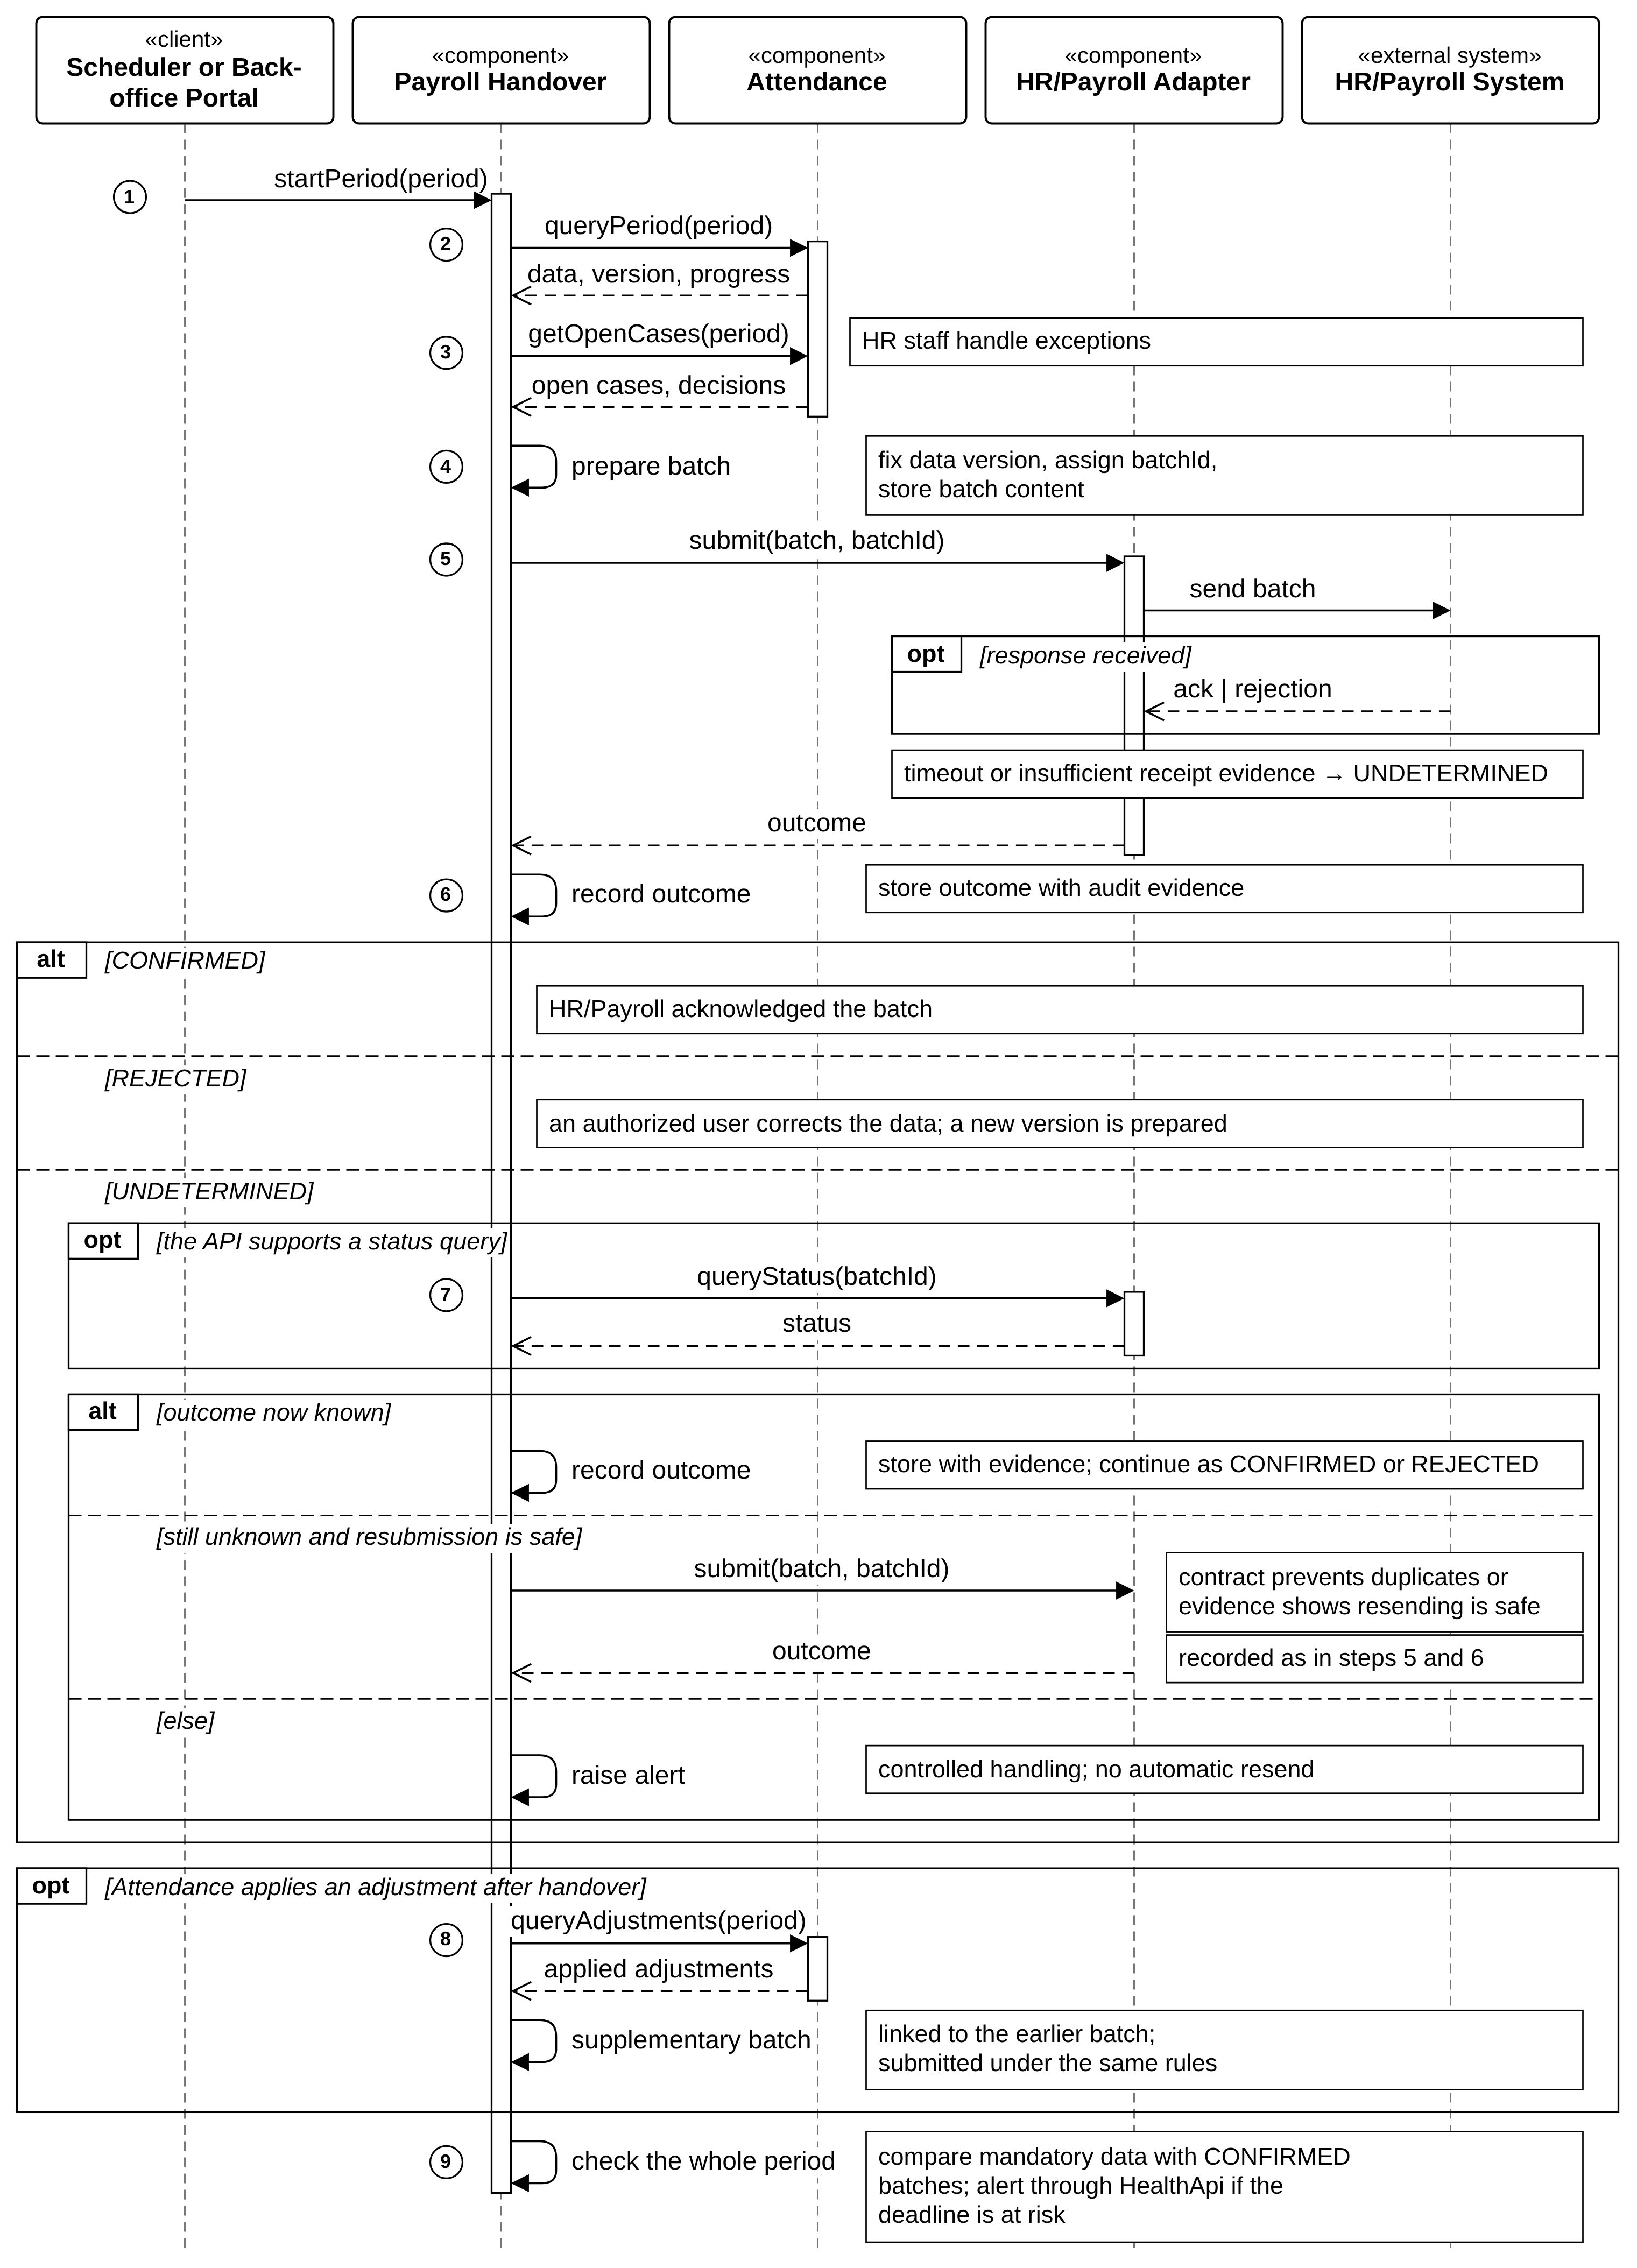
\includegraphics[width=450.0pt,height=630.0pt,keepaspectratio]{diagram/sequence/figure-4-17-payroll-handover.png}}{\fbox{\parbox{300pt}{\centering\vspace{20pt}Figure being redrawn\vspace{20pt}}}}
\par\vspace{4pt}
\textbf{Figure 4.17. Payroll Handover Sequence --- Preparation, Submission, Outcome and Supplementary Batch}\par
\phantomsection\addcontentsline{lof}{figure}{\protect\numberline{4.17}Payroll Handover Sequence --- Preparation, Submission, Outcome and Supplementary Batch}
\end{minipage}

\medskip


\Needspace{6\baselineskip}
The period follows these rules:

\begin{itemize}[leftmargin=36pt, itemsep=2pt, topsep=4pt, parsep=2pt]
  \item \textbf{Deadline (IC-01).} Data must be available at HR/Payroll before 12:00 noon on the first day of each month. We plan the first submission at 06:00 and an alert at 10:00 if the handover is still incomplete; these are checkpoints, not the final cutoff.
  \item \textbf{Shifts across a day or month.} Work Schedule Policy holds HR-approved rules for such shifts. Attendance Consolidation keeps the actual timestamps and uses these rules to assign transactions to a period. The month-end rule must be confirmed with HR before the first real handover.
  \item \textbf{Late records.} An overnight shift ending around 06:00 may not have its exit at the central site yet, so Payroll Handover checks expected shift completion, synchronization progress, and open cases before calling a period complete. It sends the available data at 06:00, marks the period incomplete, and sends later records in a linked supplementary batch, if possible before 12:00. If mandatory data is still missing at the deadline, the period stays incomplete, an alert is raised, and a later delivery is recorded as late.
  \item \textbf{Completion and deadline.} A batch acknowledgement only proves that HR/Payroll received that batch. A period is complete when all mandatory data has been handed over, and this is tracked separately from the deadline: a period can be complete but late, or on time but incomplete. Adjustments after a complete handover are not missing data.
  \item \textbf{Batch identity.} Resending unchanged content keeps its identifier and version under the contract; changed content gets a new identifier or version linked to the previous one. A batchId alone does not prove that resending is safe. A batch rejected for its content is corrected by an authorized user and sent as a new version.
\end{itemize}

\subsubsection*{4.2.5. States and Duplicate Prevention}

\phantomsection
\addcontentsline{toc}{subsubsection}{4.2.5. States and Duplicate Prevention}

The three flows rely on stored states and identifiers. NFR-02 covers only normal operation; component failures are assessed separately.

\Needspace{6\baselineskip}
Table 4.23a follows a scan up to the opening result, and Table 4.23b follows the passage and closing cycle, linked by scanId, commandId, and lane. OPEN\_CONFIRMED and CLOSED are command results; PASSAGE and LANE\_CLEAR are events. The table values are stored states. OPENED means that Gate Core has stored OPEN\_CONFIRMED.

\begin{longtable}{|>{\raggedright\arraybackslash}p{106.5pt}|>{\raggedright\arraybackslash}p{109.5pt}|>{\raggedright\arraybackslash}p{173.5pt}|}
\hline
\multicolumn{1}{|>{\columncolor{tableheader}\centering\arraybackslash}p{106.5pt}|}{\textbf{State}} & \multicolumn{1}{>{\columncolor{tableheader}\centering\arraybackslash}p{109.5pt}|}{\textbf{Meaning}} & \multicolumn{1}{>{\columncolor{tableheader}\centering\arraybackslash}p{173.5pt}|}{\textbf{Transition or Completion Conditions}} \\
\hline
\endhead
\multicolumn{3}{c}{\rule{0pt}{20pt}\normalsize\textbf{Table 4.23a. Scan States}} \\
\endlastfoot
RECEIVED & A new scan is being checked. & REJECTED if the checks fail, LANE BUSY if the lane is reserved, CANNOT PROCESS if something needed is missing, ACCEPTED if the checks pass and the atomic write succeeds. \\
\hline
LANE BUSY & The lane has an active or unresolved gate cycle. The token is not claimed. & End without a command; the employee scans again when the lane is free. \\
\hline
REJECTED & The QR code or access conditions are invalid, or the token is already claimed. & End without a command or attendance. \\
\hline
CANNOT PROCESS & Processing stopped before the command, for example because access data is unusable, ACCEPTED could not be stored, or the deadline passed before openGate. & No command is sent; the guard can start assisted access. \\
\hline
ACCEPTED & ACCEPTED is stored but there is no final outcome yet. This does not prove that no command was sent. & CANNOT PROCESS if the deadline expires before any command is sent; otherwise OPENED, CONTROLLER ERROR, or UNDETERMINED when the outcome is stored. Recover unfinished attempts from this state. \\
\hline
OPENED & The controller confirmed opening and the result is stored. This state alone does not establish passage or attendance. & Return the result to the kiosk. Missing passage after 15 seconds, or an emergency without passage evidence, leads to PENDING RECONCILIATION. \\
\hline
CONTROLLER ERROR & The controller explicitly confirmed that it did not open. & End without attendance; release the lane once the controller reports it ready. \\
\hline
UNDETERMINED & No reliable evidence of what the controller did. & Inquire if possible and move to the matching state; otherwise PENDING RECONCILIATION. Never resend the command to test. \\
\hline
PENDING RECONCILIATION & Not enough evidence for automatic attendance. & RECONCILED once Gate Core stores the authorized conclusion; earlier evidence is kept. \\*
\hline\noalign{\nobreak}
RECONCILED & Gate Core has stored the conclusion. & Send the acknowledgement; Attendance Review tracks the attendance change separately. \\
\hline
\end{longtable}
\phantomsection\addcontentsline{lot}{table}{\protect\numberline{4.23a}Scan States}


If the database cannot be written at all, RECEIVED and CANNOT PROCESS exist only as response states.

\Needspace{6\baselineskip}
Gate Core stores passageStatus and closureStatus separately, because the controller may end an opening opportunity before the 15-second passage observation ends. The observation timer starts at OPEN\_CONFIRMED and only flags a missing passage for review; it never permits closeGate.

\begin{longtable}{|>{\raggedright\arraybackslash}p{77pt}|>{\raggedright\arraybackslash}p{116pt}|>{\raggedright\arraybackslash}p{198pt}|}
\hline
\multicolumn{1}{|>{\columncolor{tableheader}\centering\arraybackslash}p{77pt}|}{\textbf{Track}} & \multicolumn{1}{>{\columncolor{tableheader}\centering\arraybackslash}p{116pt}|}{\textbf{Stored state}} & \multicolumn{1}{>{\columncolor{tableheader}\centering\arraybackslash}p{198pt}|}{\textbf{Transition and action}} \\
\hline
\endhead
\multicolumn{3}{c}{\rule{0pt}{20pt}\normalsize\textbf{Table 4.23b. Gate-Cycle States}} \\
\endlastfoot
Passage & WAITING & Set on OPEN\_CONFIRMED; wait for a PASSAGE event for this command and lane. \\
\hline
Passage & PASSED & For a timely, reliable QR passage while the scan is still OPENED, store the event and at most one original attendance transaction per scanId together. If already sent to reconciliation, for example by an emergency release, keep passage evidence for review without automatic attendance. Assisted cases still require HR approval. \\
\hline
Passage & NO\_PASSAGE & No reliable PASSAGE within 15 seconds; open a reconciliation case. A PASSAGE that arrives later is stored once with an audit record and marked LATE\_PASSAGE. It creates no attendance automatically; Attendance Review decides. It does not restart the 15-second timer or close the gate. \\
\hline
Closure & OPENED & Set on OPEN\_CONFIRMED; wait for LANE\_CLEAR. \\
\hline
Closure & CLEAR\_TO\_CLOSE & LANE\_CLEAR stored; one close command reserved. \\
\hline
Closure & CLOSE\_SENT & Persist closeCommandId before dispatch; the command may have been sent. Repeated events query that command rather than sending another. \\
\hline
Closure & CLOSED & Controller confirmed closing; the lane is released. Attendance is not affected. \\
\hline
Closure & CLOSE\_FAILED / CLOSE\_UNCERTAIN & Store the failure or unknown result and alert the guard; never claim CLOSED. The lane stays reserved until a query confirms CLOSED or a guard restores a safe state. \\*
\hline\noalign{\nobreak}
Emergency & EMERGENCY\_HOLD & Block normal closing and new scans on the lane until an authorized reset is confirmed, then follow the normal closing rule. \\
\hline
\end{longtable}
\phantomsection\addcontentsline{lot}{table}{\protect\numberline{4.23b}Gate-Cycle States}


\Needspace{6\baselineskip}
A few rules connect these states:

\begin{itemize}[leftmargin=36pt, itemsep=2pt, topsep=4pt, parsep=2pt]
  \item \textbf{Order.} Up to the stored opening result there is one sequence: check conditions; atomically reserve the lane, claim the token, and store ACCEPTED; send the opening command; store the outcome. Once the confirmed opening is stored, returning the kiosk result, recording passage, and closing safely run independently, each on its own signal: closing never waits for passage, and attendance never waits for closing or for the kiosk.
  \item \textbf{Timeouts.} If the station times out, it shows UNDETERMINED and calls getScanStatus with the same scanId instead of starting a new scan. Each request carries a deadline: Gate Transaction Processor does not start a command for an expired request, but it still checks a command that may already have been sent. If the deadline runs out after ACCEPTED but before openGate, nothing reached the controller, so the lane is released while the token stays claimed (Table 4.22).
  \item \textbf{History.} An approved adjustment is linked to the original scan and never overwrites it. Attendance Consolidation links an existing transaction or records a traceable adjustment instead of creating a second entry or exit, and late or conflicting passage evidence stays available for review.
  \item \textbf{No reliable PASSAGE signal.} The I-07 rule cannot run. An independent passage sensor must be verified first; until then, attendance comes from evidenced assisted records approved by HR.
  \item \textbf{Recovery.} Gate Transaction Processor reviews uncertain openings and OPENED scans awaiting passage or closure, queries the controller where supported, and otherwise sends the case to reconciliation or alerts the guard as in Table 4.22. Site Sync redelivers unacknowledged events with their original identifiers. Access Decision uses Eligibility Snapshot only under the version, continuity, and freshness conditions of degraded mode (I-10), and marks each degraded decision for review after reconnection.
\end{itemize}

\Needspace{6\baselineskip}
Table 4.24 lists the identifiers that keep scans, commands, events, and batches apart. A scan can produce several events, and a redelivered event keeps its eventId.

\begin{longtable}{|>{\raggedright\arraybackslash}p{95pt}|>{\raggedright\arraybackslash}p{120pt}|>{\raggedright\arraybackslash}p{190pt}|}
\hline
\multicolumn{1}{|>{\columncolor{tableheader}\centering\arraybackslash}p{95pt}|}{\textbf{Identifier}} & \multicolumn{1}{>{\columncolor{tableheader}\centering\arraybackslash}p{120pt}|}{\textbf{Owner}} & \multicolumn{1}{>{\columncolor{tableheader}\centering\arraybackslash}p{190pt}|}{\textbf{Use}} \\
\hline
\endhead
\multicolumn{3}{c}{\rule{0pt}{20pt}\normalsize\textbf{Table 4.24. Identifiers Used across the Main Flows}} \\
\endlastfoot
scanId & Station Client & One scan and its status inquiries. \\
\hline
commandId & Gate Transaction Processor & Links each opening or closing command to its result; it does not by itself prevent duplicate execution. \\
\hline
passageEventId & Turnstile controller & Stable identifier for a passage event, linked to the lane and opening command under I-01. \\
\hline
tokenId & QR Credential Issuance & Identifies a QR code under the proposed single-use policy. \\
\hline
eventId & Event producer & Identifies a transferred event and remains the same on retry. \\
\hline
Version or sequence & Owning data source & Detects missing or out-of-order updates. \\
\hline
supportCaseId & Gate Intervention & Links an assistance case to its evidence and scan, when present. \\
\hline
Decision ID and version & Attendance Review & Tracks approval and safe repeated application. \\*
\hline\noalign{\nobreak}
batchId and version & Payroll Handover & Tracks a handover, retry, or supplementary batch. \\
\hline
\end{longtable}
\phantomsection\addcontentsline{lot}{table}{\protect\numberline{4.24}Identifiers Used across the Main Flows}


\Needspace{6\baselineskip}
The identifiers prevent three kinds of duplicates:

\begin{itemize}[leftmargin=36pt, itemsep=2pt, topsep=4pt, parsep=2pt]
  \item \textbf{Duplicate events.} Each receiver stores the business change and an event-processed marker together, and returns the stored outcome when the same event arrives again.
  \item \textbf{Duplicate attendance.} Gate Transaction Processor accepts each passageEventId once and creates at most one original QR transaction per scanId; a second, different passage is kept as an anomaly. Attendance Consolidation checks the scan link again when it receives transactions or applies decisions.
  \item \textbf{QR replay.} The token is claimed in the same atomic write as ACCEPTED; Access Decision only verifies it. A unique-token constraint only works within the store that enforces it, and finding a duplicate after the gate has opened is only anomaly detection.
\end{itemize}

\Needspace{6\baselineskip}
Table 4.25 lists the handover batch states used in Flow C.

\begin{longtable}{|>{\raggedright\arraybackslash}p{108.5pt}|>{\raggedright\arraybackslash}p{129.5pt}|>{\raggedright\arraybackslash}p{171.5pt}|}
\hline
\multicolumn{1}{|>{\columncolor{tableheader}\centering\arraybackslash}p{108.5pt}|}{\textbf{State}} & \multicolumn{1}{>{\columncolor{tableheader}\centering\arraybackslash}p{129.5pt}|}{\textbf{Meaning}} & \multicolumn{1}{>{\columncolor{tableheader}\centering\arraybackslash}p{171.5pt}|}{\textbf{Handling}} \\
\hline
\endhead
\multicolumn{3}{c}{\rule{0pt}{20pt}\normalsize\textbf{Table 4.25. Handover Batch States}} \\
\endlastfoot
PREPARED & Batch content and identity have been stored. & Submit through HR/Payroll Adapter. \\
\hline
SENT & A submission has occurred; the outcome is being determined. & Track acknowledgements or errors. \\
\hline
CONFIRMED & Receipt evidence that satisfies I-02. & Store the acknowledgement and update period progress. \\
\hline
REJECTED & HR/Payroll clearly refused the content. & Handle within authority and create a new version. \\*
\hline\noalign{\nobreak}
UNDETERMINED & A timeout, or a response without enough receipt evidence. & Inquire, resubmit when safe, or route for controlled handling. \\
\hline
\end{longtable}
\phantomsection\addcontentsline{lot}{table}{\protect\numberline{4.25}Handover Batch States}


\Needspace{9\baselineskip}
\subsection*{4.3. Class Responsibilities for the Gate Flow}

\phantomsection
\addcontentsline{toc}{subsection}{4.3. Class Responsibilities for the Gate Flow}


The proposed classes for the gate flow keep the scan, the controller command, the gate cycle, the passage evidence, and the attendance transaction apart:

\begin{itemize}[leftmargin=36pt, itemsep=2pt, topsep=4pt, parsep=2pt]
  \item \textbf{StationClient} submits a scan through GateCoreApi.
  \item \textbf{GateTransactionProcessor} checks the existing ScanAttempt, asks AccessDecision to evaluate the QR code against EligibilitySnapshot, and stores the ACCEPTED attempt, its TokenReservation, and a new GateCycle for the lane in one transaction before calling the controller port.
  \item \textbf{GateCommand} carries a commandId linked to its scan or support case and lane.
  \item The \textbf{TurnstileAdapter} class implements the turnstile command ports (IOpenGate, ICloseGate, IEmergencyGate) and reports PASSAGE and LANE\_CLEAR through IPassageEvents. A receipt stays internal to the adapter. For openGate, the final outcome is OPEN\_CONFIRMED, CONTROLLER ERROR (confirmed non-execution), or UNDETERMINED.
  \item \textbf{GateCycle} holds the passage and closure states, the 15-second observation deadline, the lane-clear signal, and the close command. While a lane has an active or unresolved GateCycle, the lane is busy.
  \item \textbf{PassageEvent} is stored before \textbf{AttendanceTransaction} is created. The data model allows at most one original transaction per scanId and accepts each passageEventId once.
\end{itemize}

The class diagrams below are drawn from the Task 2 code (Chapter 9), so the names are the ones in \code{src/tmc_gate}. In all three figures a solid arrow means that a class uses another one, a dashed arrow with a hollow triangle means that it implements an interface, a solid line with a hollow triangle means that an interface extends another one, and interface names are in italics. Only the operations needed to follow the flow are shown.

\Needspace{12\baselineskip}
\subsubsection*{4.3.1. Scan Flow}

\phantomsection
\addcontentsline{toc}{subsubsection}{4.3.1. Scan Flow}

\noindent\begin{minipage}{\linewidth}
\centering
\IfFileExists{diagram/class/figure-4-18-scan-flow-classes.png}{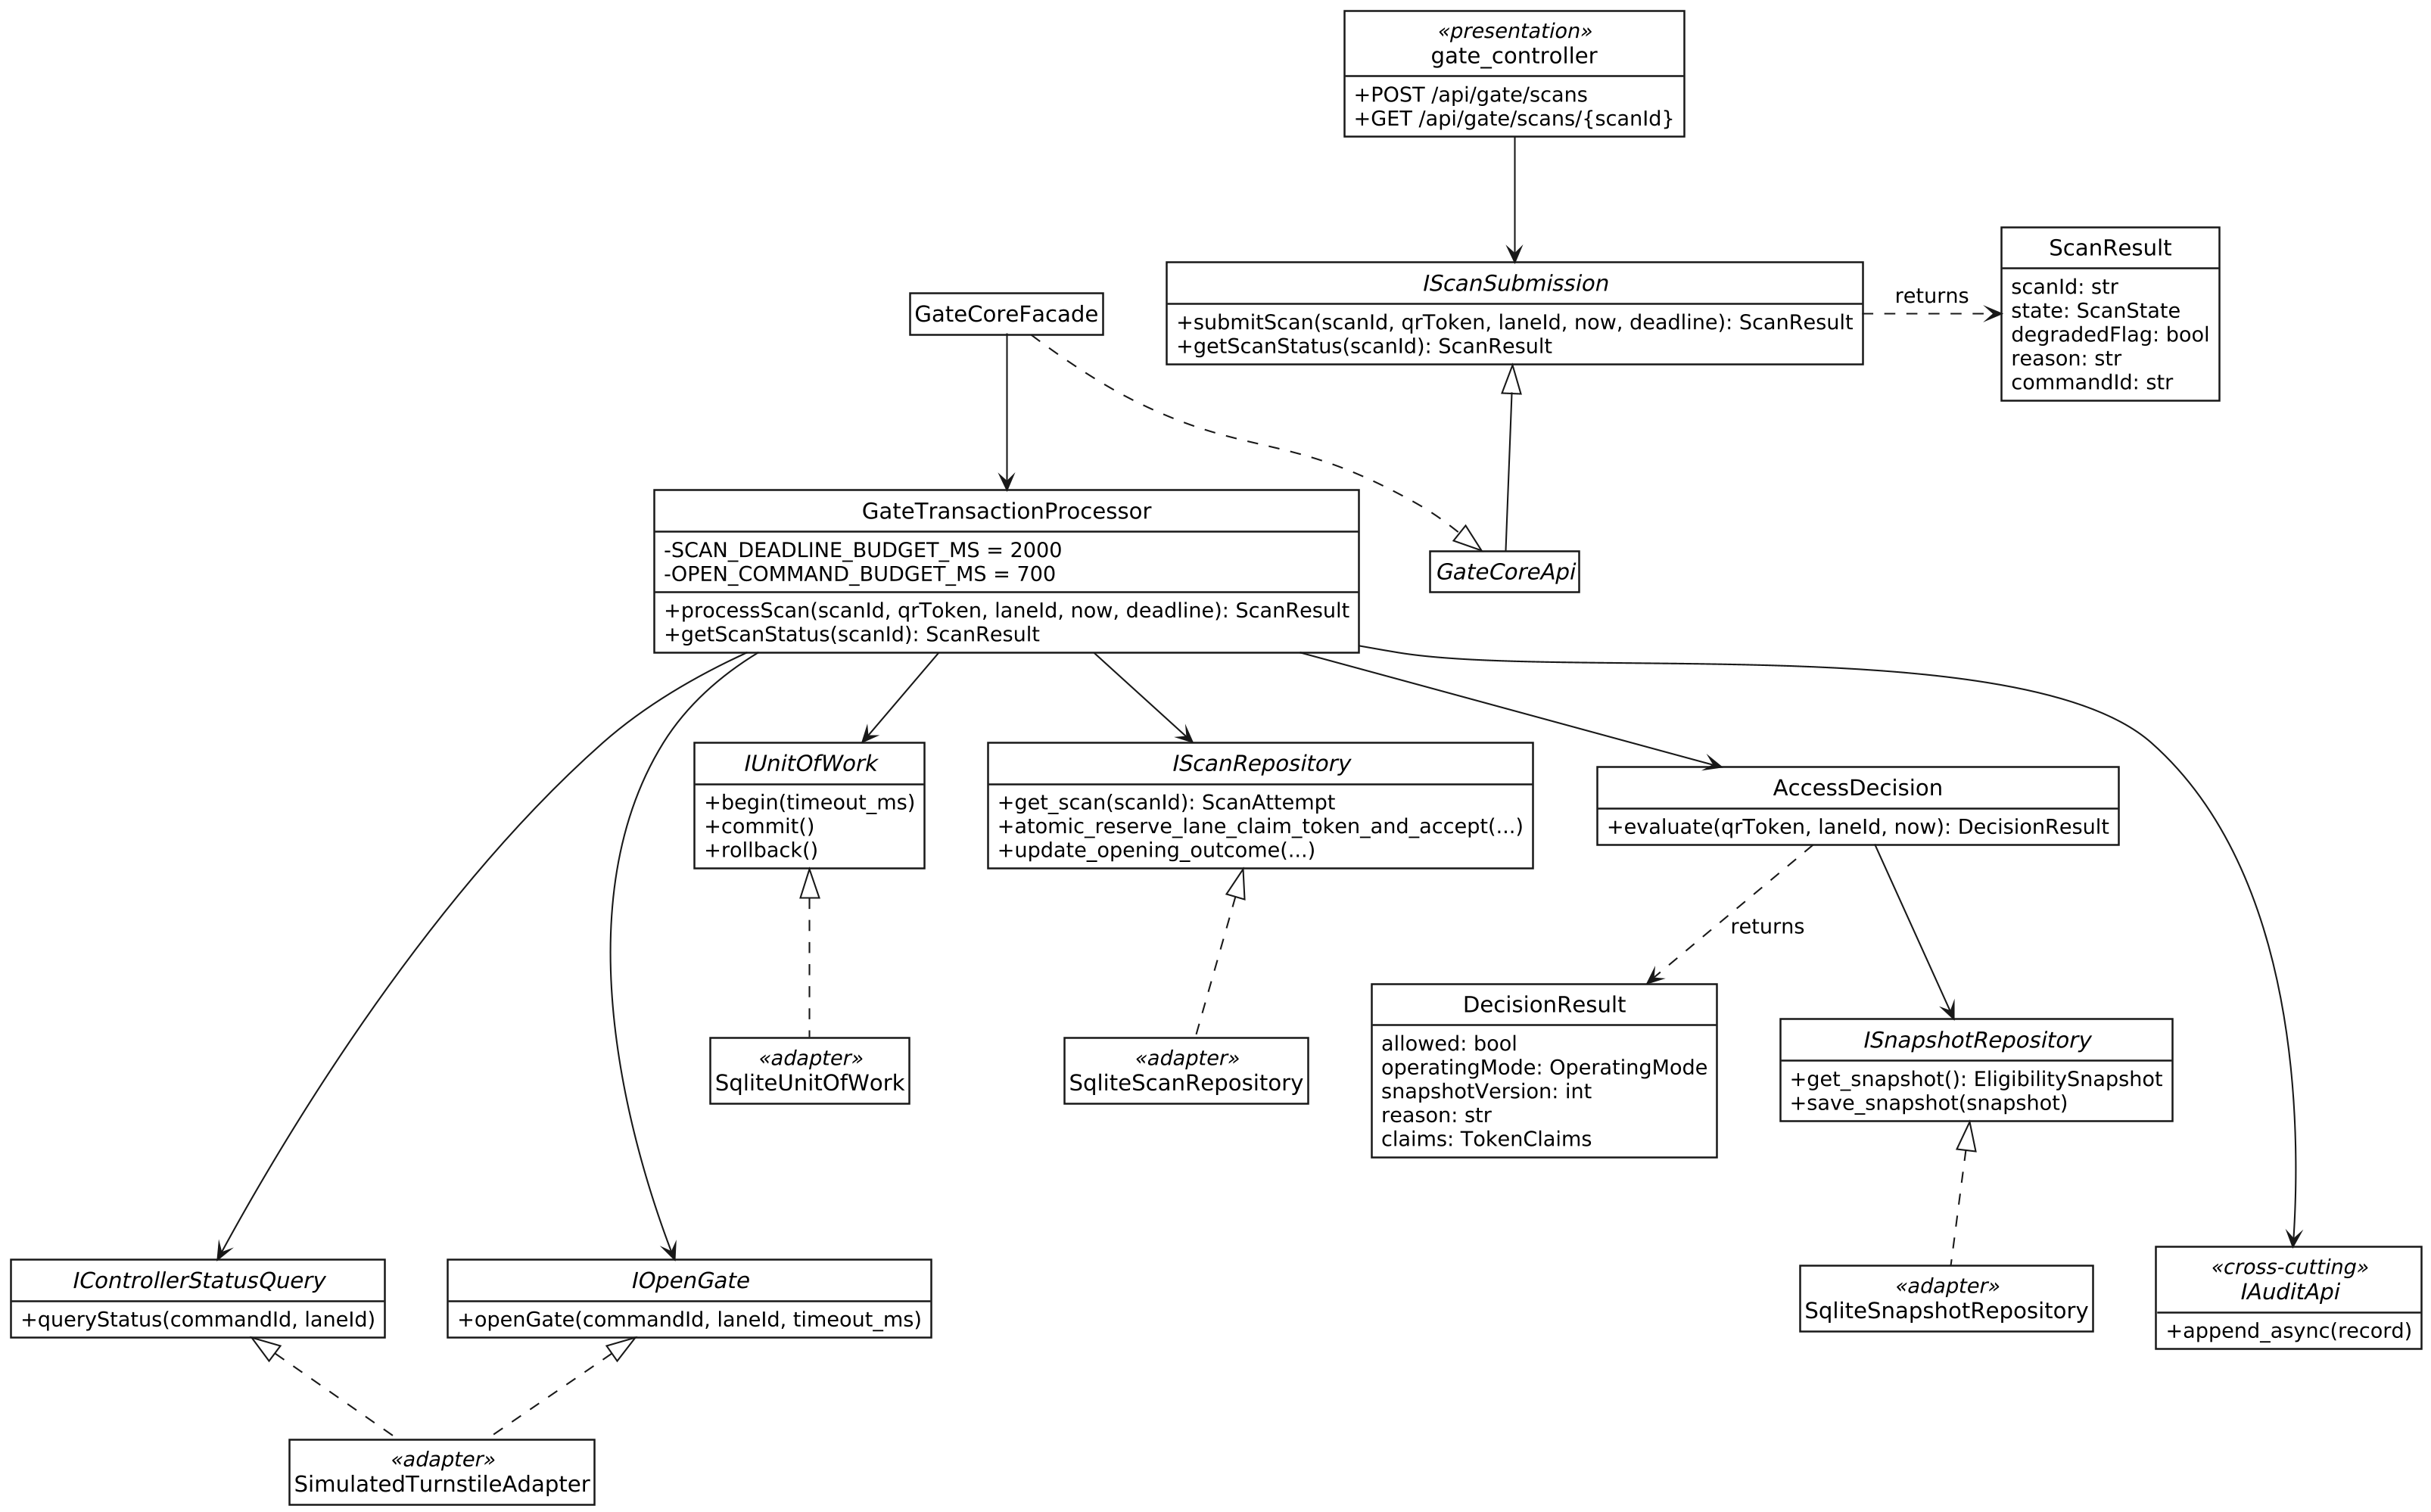
\includegraphics[width=\linewidth,height=330pt,keepaspectratio]{diagram/class/figure-4-18-scan-flow-classes.png}}{\fbox{\parbox{300pt}{\centering\vspace{20pt}Figure being redrawn\vspace{20pt}}}}

\vspace{6pt}
\textbf{Figure 4.18. Class Diagram of the Scan Flow}
\phantomsection\addcontentsline{lof}{figure}{\protect\numberline{4.18}Class Diagram of the Scan Flow}
\end{minipage}

\vspace{10pt}

Figure 4.18 shows the classes behind a QR scan (Flow A). The kiosk route in the \code{gate_controller} router only knows IScanSubmission. GateCoreFacade implements it through GateCoreApi and hands the scan to GateTransactionProcessor, which is the only class that coordinates the flow. The processor asks AccessDecision for the decision, and AccessDecision reads the EligibilitySnapshot through ISnapshotRepository. Every other dependency of the processor is an interface: IScanRepository and IUnitOfWork for the transaction, IOpenGate and IControllerStatusQuery for the controller, and IAuditApi for audit evidence. All of them are passed in through the constructor in \code{app.py}.

The two budgets in the processor come from Table 5.5: the whole scan must finish within 2 seconds, and openGate gets at most 700 ms of that time. The processor stores the ACCEPTED scan, its TokenReservation, and the new GateCycle in one transaction before it sends openGate, so a crash after the command still leaves evidence that the lane is taken.

\Needspace{12\baselineskip}
\subsubsection*{4.3.2. Controller Signals and Gate Intervention}

\phantomsection
\addcontentsline{toc}{subsubsection}{4.3.2. Controller Signals and Gate Intervention}

\noindent\begin{minipage}{\linewidth}
\centering
\IfFileExists{diagram/class/figure-4-19-signals-intervention-classes.png}{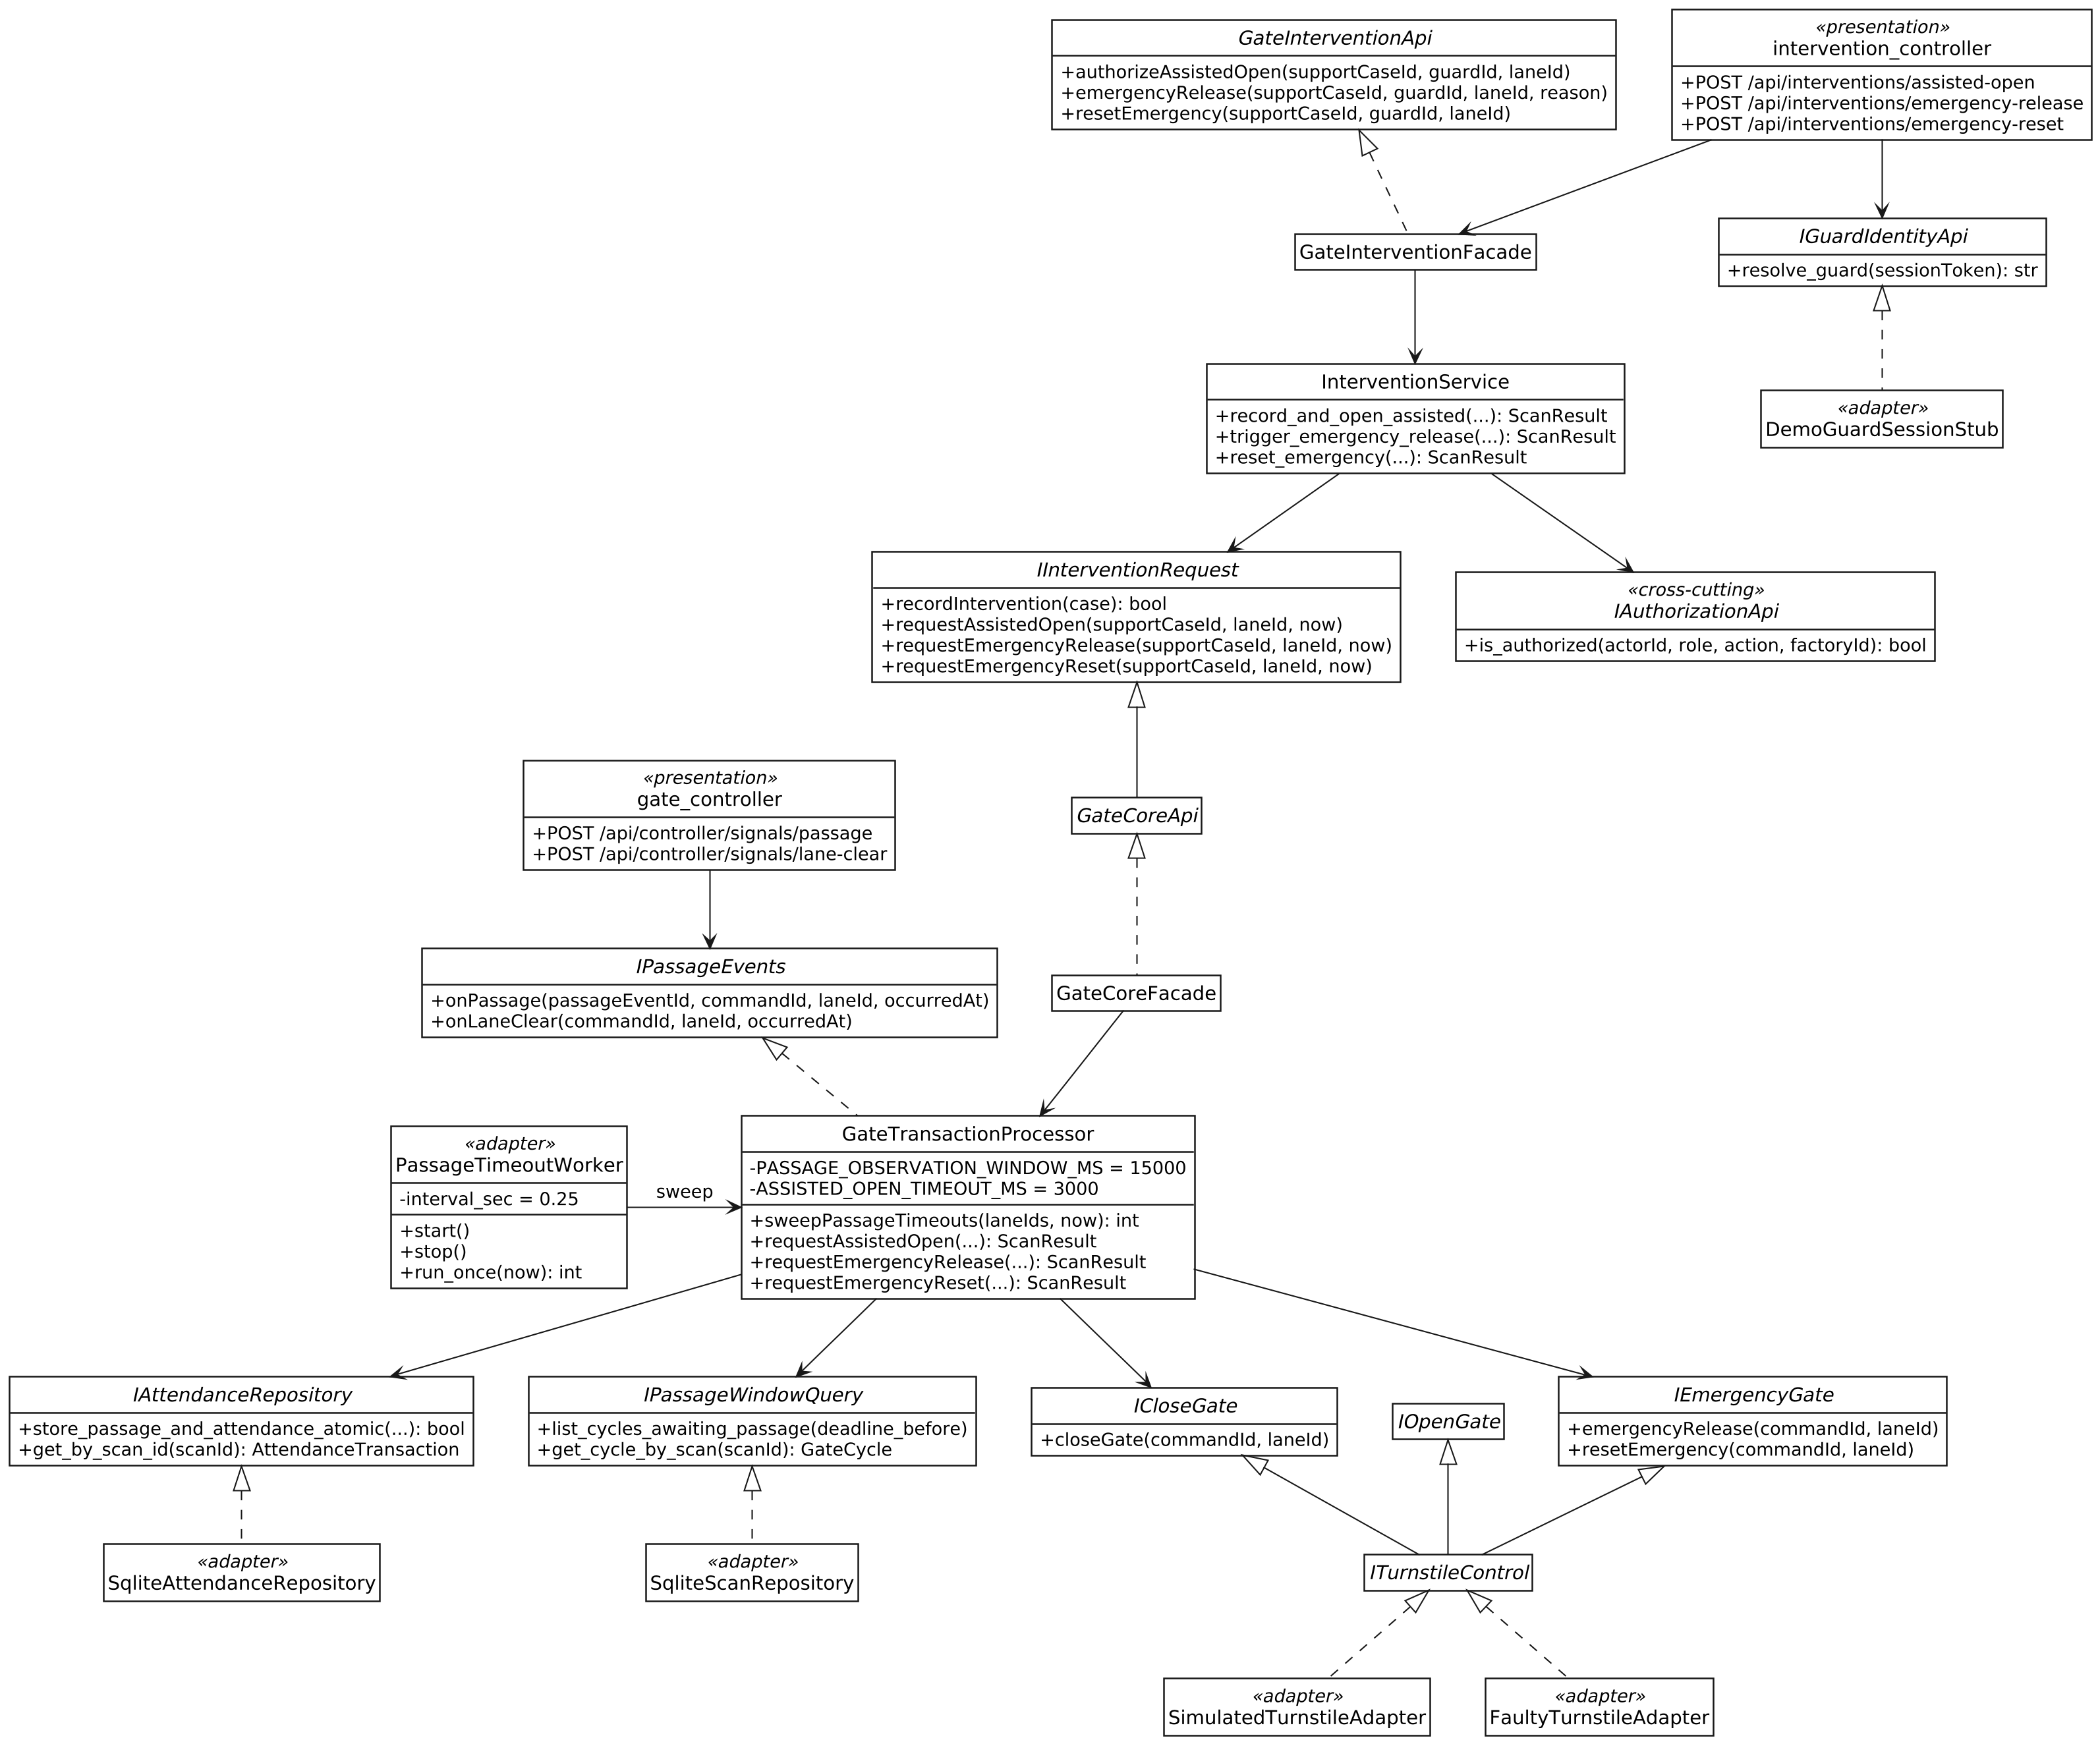
\includegraphics[width=\linewidth,height=420pt,keepaspectratio]{diagram/class/figure-4-19-signals-intervention-classes.png}}{\fbox{\parbox{300pt}{\centering\vspace{20pt}Figure being redrawn\vspace{20pt}}}}

\vspace{6pt}
\textbf{Figure 4.19. Class Diagram of Controller Signals and Gate Intervention}
\phantomsection\addcontentsline{lof}{figure}{\protect\numberline{4.19}Class Diagram of Controller Signals and Gate Intervention}
\end{minipage}

\vspace{10pt}

Figure 4.19 shows the other ways into Gate Core. PASSAGE and LANE\_CLEAR from the controller arrive at \code{gate_controller} and go to GateTransactionProcessor through IPassageEvents. PassageTimeoutWorker calls sweepPassageTimeouts every 0.25 seconds. The processor then uses IPassageWindowQuery to find the cycles whose 15-second window has ended. This timer never sends closeGate.

Guard actions (Flow B) take a separate path. \code{intervention_controller} gets the guard from the session through IGuardIdentityApi, and InterventionService checks the guard's authority through IAuthorizationApi before it calls Gate Core. InterventionService only sees IInterventionRequest, not the whole GateCoreApi, which is the ISP split of Section 7.1. The turnstile ports are also split: one adapter class implements ITurnstileControl, but the processor depends on IOpenGate, ICloseGate, and IEmergencyGate one by one. FaultyTurnstileAdapter is a second implementation that the contract tests use to check the LSP rule (Section 9.4).

\Needspace{12\baselineskip}
\subsubsection*{4.3.3. Gate Core Entities}

\phantomsection
\addcontentsline{toc}{subsubsection}{4.3.3. Gate Core Entities}

\noindent\begin{minipage}{\linewidth}
\centering
\IfFileExists{diagram/class/figure-4-20-gate-core-entities.png}{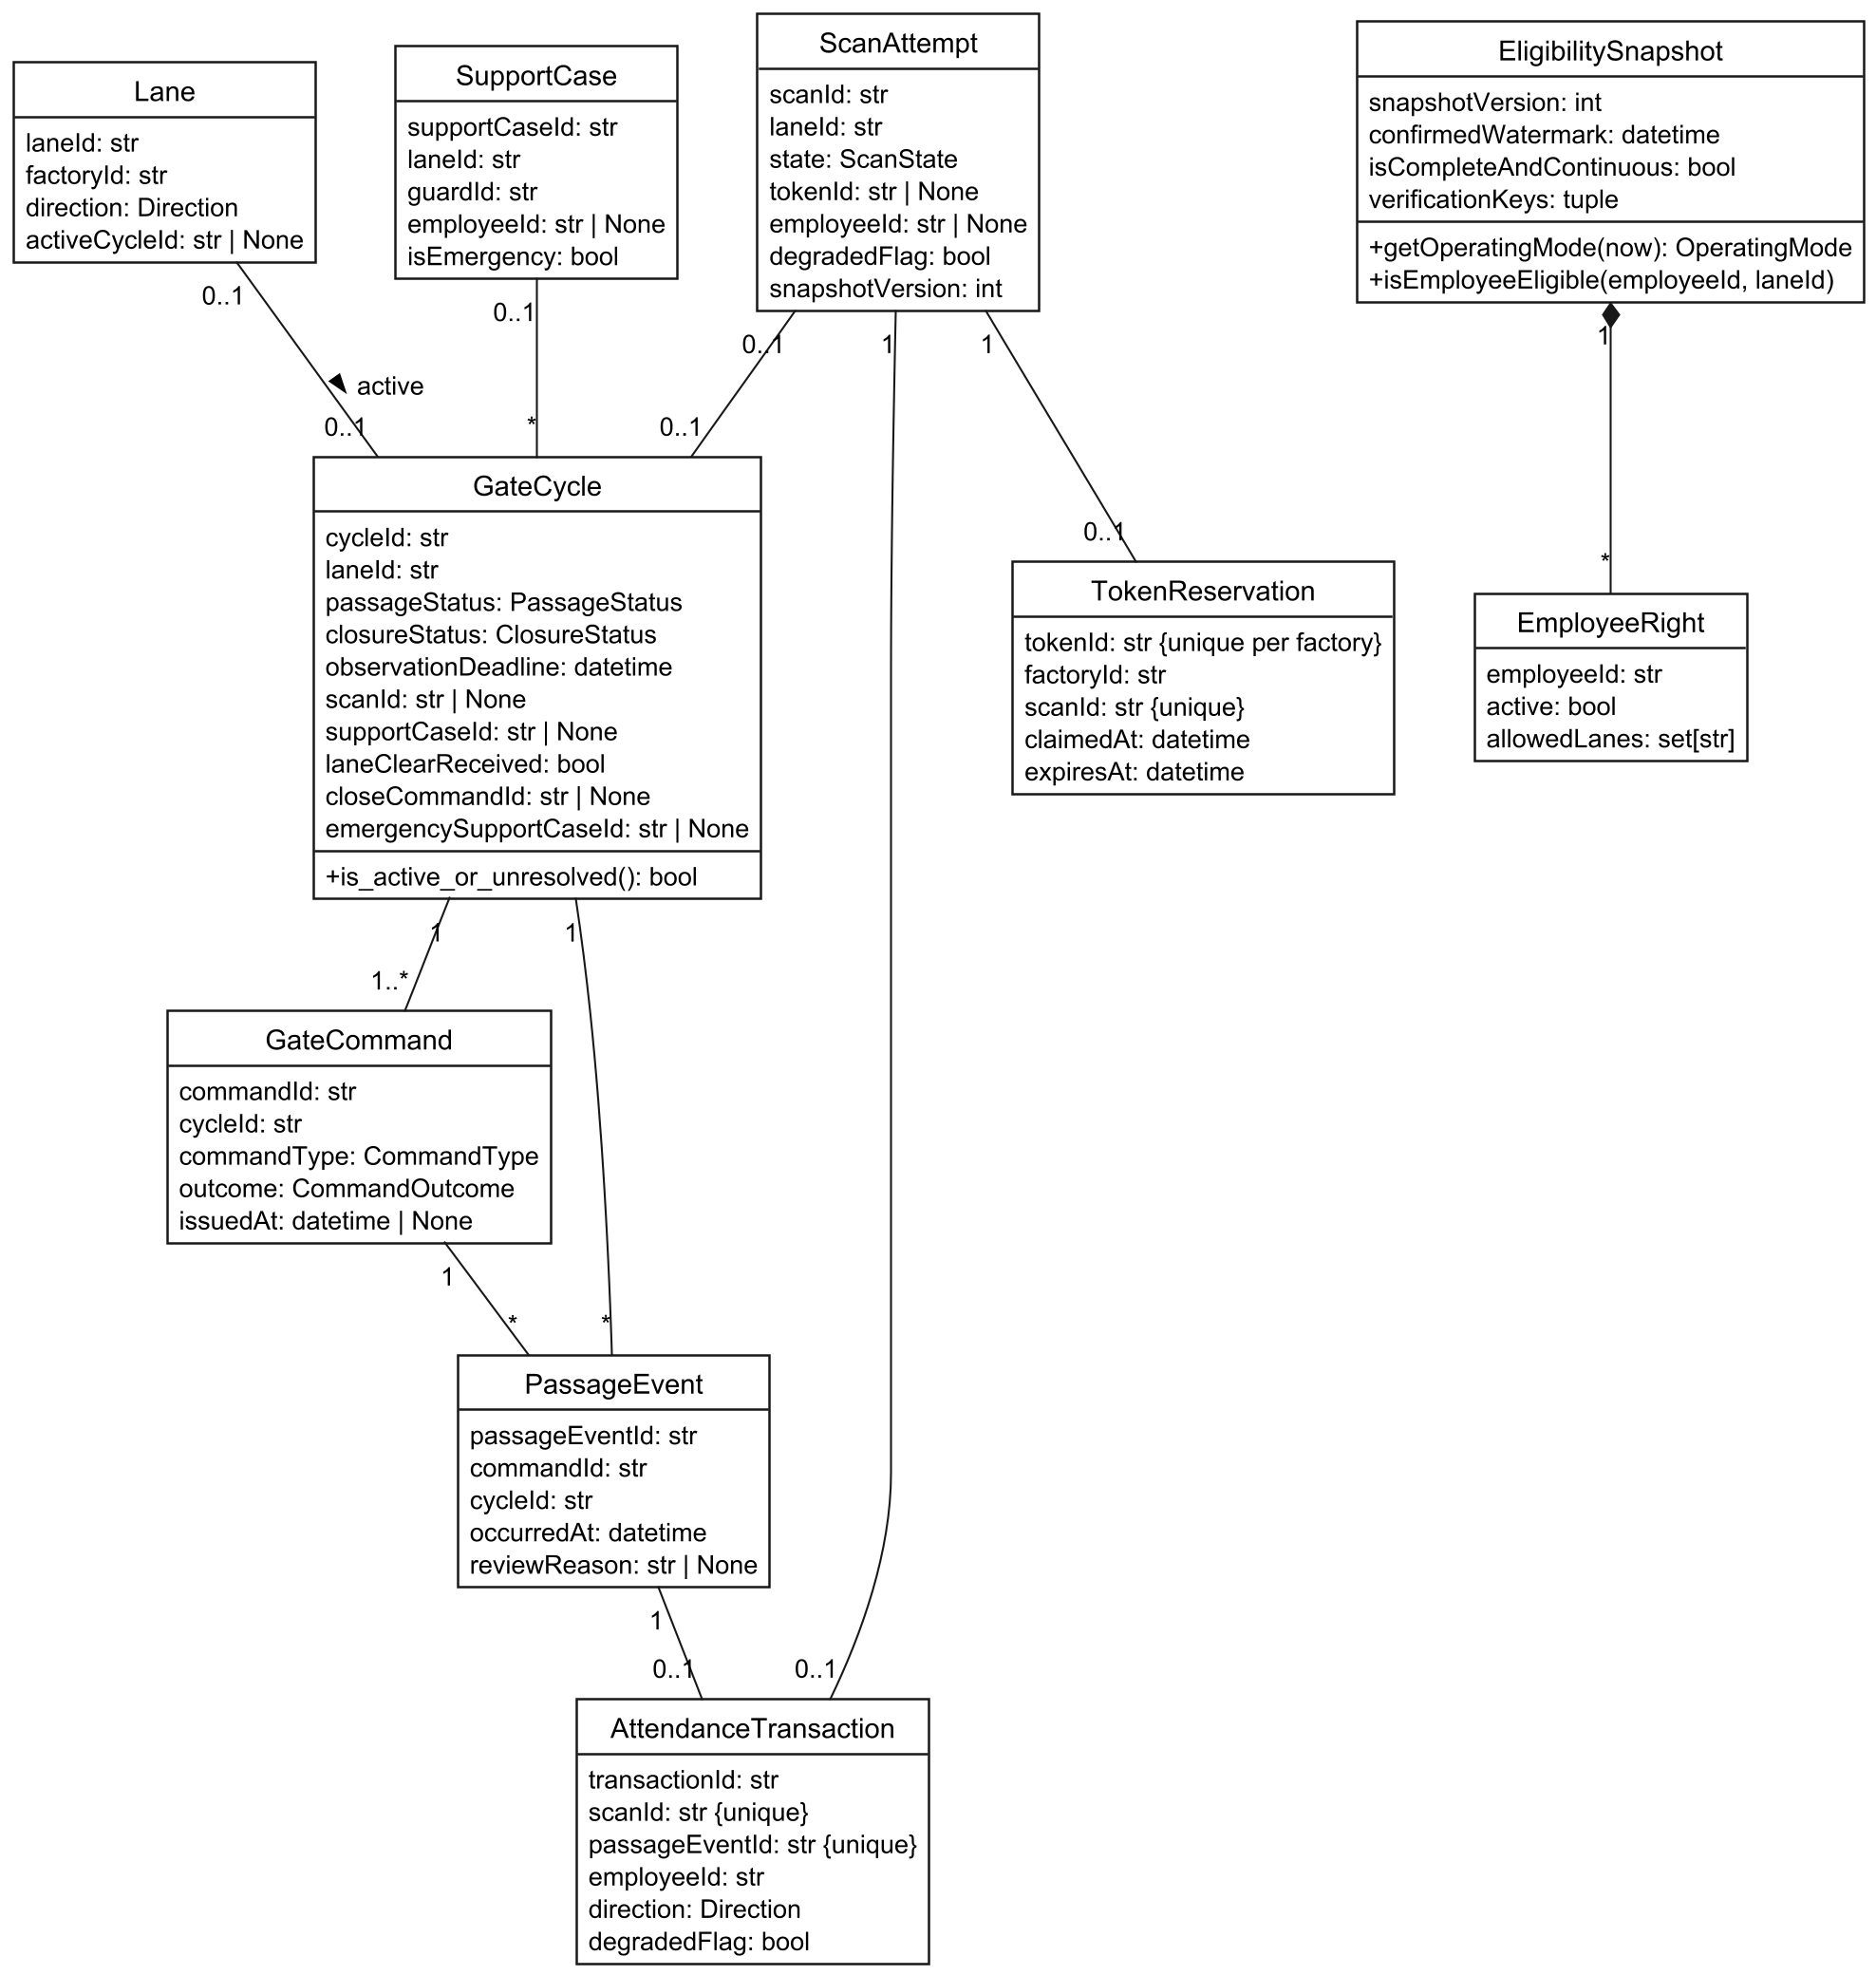
\includegraphics[width=\linewidth,height=420pt,keepaspectratio]{diagram/class/figure-4-20-gate-core-entities.png}}{\fbox{\parbox{300pt}{\centering\vspace{20pt}Figure being redrawn\vspace{20pt}}}}

\vspace{6pt}
\textbf{Figure 4.20. Gate Core Entities and Their Multiplicities}
\phantomsection\addcontentsline{lof}{figure}{\protect\numberline{4.20}Gate Core Entities and Their Multiplicities}
\end{minipage}

\vspace{10pt}

Figure 4.20 shows the entities and their multiplicities, including the rule that a Lane has at most one active GateCycle. A later close failure never erases a confirmed attendance transaction, and neither assisted nor emergency opening creates attendance from the opening alone.

Table 4.26 lists the enumerations that appear as attribute types in Figures 4.18 to 4.20. The values are the ones in \code{src/tmc_gate/domain/enums.py}.

\begin{longtable}{|>{\raggedright\arraybackslash}p{92pt}|>{\raggedright\arraybackslash}p{178pt}|>{\raggedright\arraybackslash}p{141pt}|}
\hline
\multicolumn{1}{|>{\columncolor{tableheader}\centering\arraybackslash}p{92pt}|}{\textbf{Type}} & \multicolumn{1}{>{\columncolor{tableheader}\centering\arraybackslash}p{178pt}|}{\textbf{Values}} & \multicolumn{1}{>{\columncolor{tableheader}\centering\arraybackslash}p{141pt}|}{\textbf{Used in}} \\
\hline
\endhead
\multicolumn{3}{c}{\rule{0pt}{20pt}\normalsize\phantomsection\addcontentsline{lot}{table}{\protect\numberline{4.26}Value Types Used in the Class Diagrams}\textbf{Table 4.26. Value Types Used in the Class Diagrams}} \\
\endlastfoot
ScanState & RECEIVED, ACCEPTED, OPENED, REJECTED, LANE\_BUSY, CANNOT\_PROCESS, CONTROLLER\_ERROR, UNDETERMINED, PENDING\_RECONCILIATION, RECONCILED & \code{ScanAttempt.state} \\
\hline
PassageStatus & WAITING, PASSED, NO\_PASSAGE & \code{GateCycle.passageStatus} \\
\hline
ClosureStatus & OPENED, CLEAR\_TO\_CLOSE, CLOSE\_SENT, CLOSED, CLOSE\_FAILED, CLOSE\_UNCERTAIN, EMERGENCY\_HOLD & \code{GateCycle.closureStatus} \\
\hline
CommandType & OPEN, CLOSE, EMERGENCY\_RELEASE, RESET & \code{GateCommand.commandType} \\
\hline
CommandOutcome & SENT, NOT\_SENT, OPEN\_CONFIRMED, CLOSED, EMERGENCY\_RELEASED, RESET\_CONFIRMED, CONTROLLER\_ERROR, UNDETERMINED & \code{GateCommand.outcome}; SENT and NOT\_SENT are stored states only, a port never returns them \\
\hline
OperatingMode & NORMAL, DEGRADED, CANNOT\_PROCESS & Result of \code{EligibilitySnapshot.getOperatingMode} (Figure 5.3) \\*
\hline\noalign{\nobreak}
Direction & ENTRY, EXIT & direction of Lane and of AttendanceTransaction \\
\hline
\end{longtable}
